\section{Background Estimation}%
\label{sec:background_estimation}

The dominant background processes in the search for Higgs boson pair production
in $\bbtautau$ final states are \Zjets, \ttbar, and backgrounds with quark- or
gluon-initiated jets that are misidentified as \tauhadvis (\faketauhadvis
backgrounds).
% Backgrounds with \faketauhadvis primarily originate from multi-jet, \Wjets,
% and \ttbar processes.
Minor backgrounds originate from single-top, $\ttbar V$, diboson, and single
Higgs boson production.  The single Higgs boson production modes considered in
this search are \ggF, VBF, \VH and \ttH for $H \to \tautau$; $\VH$ and $\ttH$
for $H \to \bbbar$. Single Higgs boson production via $\bbbar H$ is found to be
negligible.
% While single Higgs boson production is classified as a minor background here,
% it has relevance to the extraction of \HH signals due to their similar
% signatures.

The \Zjets and \ttbar backgrounds are estimated using templates obtained from
simulation with their normalisations being determined in a simultaneous
likelihood fit to observed data in SRs and CRs. A CR enriched in $Z$~boson
production in association with jets from quarks of heavy flavour (\ZHF) is
defined in \Cref{sec:bkg_zjets} providing constraints on the normalisation of
this background. The normalisation of the \ttbar background is constrained by
the inclusion of the SR of the \lephad SLT channel and the \ZHF CR in the
simultaneous fit, both having a measurable contribution of events from \ttbar
production.
% The SR of the \lephad SLT channel serves to constrain the
% normalisation of the \ttbar background as it selects \ttbar with high purity.

Major \faketauhadvis backgrounds are estimated using (semi-)data-driven methods,
while minor ones are estimated using simulation. In the \hadhad channel, the
primary sources of \faketauhadvis are \ttbar and multi-jet production for which
separate estimation techniques are used. The \faketauhadvis background from
\ttbar (\ttbarFakes) is estimated using simulation after applying corrections of
\jettotauhadvis misidentification efficiencies measured in a CR. This method is
described in \Cref{sec:bkg_hadhad_ttbarfakes}. The multi-jet background is
estimated using a fully data-driven \emph{fake factor method} that is introduced
in \Cref{sec:bkg_hadhad_ff}. Both methods were developed as part of this thesis
and differ from the approach adopted in the previous publication in this
channel~\cite{HIGG-2016-16-witherratum}. Lastly, the estimation of the
\faketauhadvis backgrounds in the \lephad channels uses a \emph{combined fake
  factor method} that simultaneously estimates \faketauhadvis backgrounds from
multi-jet and \ttbar processes. This method is briefly summarised
in~\Cref{sec:bkg_lephad_combined_ff}.

Minor background contributions are estimated using simulation and are normalised
to the integrated luminosity of the \pp~collision dataset using the highest
order cross section predictions available. These backgrounds are not discussed
in detail in this section, however, theoretical uncertainties on the modelling
of these processes using simulation are discussed in
\Cref{sec:modelling_uncertainties}.

\subsection{Associated Production of $\PZ \to \ell\ell$ with Quarks of Heavy Flavour}%
\label{sec:bkg_zjets}
% References:
%
% PMG weak boson wiki
% https://twiki.cern.ch/twiki/bin/view/AtlasProtected/PmgWeakBosonProcesses#Normalisation_discrepancies_due
%
% Differential cross-sections for Z + b-jets at 13 TeV
% https://link.springer.com/content/pdf/10.1007/JHEP07(2020)044.pdf

The production of \PZ bosons in association with jets is estimated
using events simulated with \SHERPA[2.2.1]~\cite{Bothmann:2019yzt}
interfaced to the matrix element generators
\OPENLOOPS~\cite{Buccioni:2019sur,Cascioli:2011va,Denner:2016kdg} and
Comix~\cite{Gleisberg:2008fv} (cf.\ \Cref{tab:monte_carlo} in
\Cref{sec:data_and_simulation}). This generator configuration merges
hard-scatter matrix elements at NLO for final states with up to two
partons with matrix elements at LO for up to four partons. Prior to
the fit, inclusive \Zjets cross sections at
NNLO~\cite{Anastasiou:2003ds} are used for the normalisation of the
background prediction.

% Why IS HF difficult?
% Theory context here: https://arxiv.org/pdf/2204.12355.pdf
The requirement of having two \btagged jets in the signal regions
leads to an enhancement of \PZ bosons produced in association with
quarks of heavy flavour. The modelling of the \ZHF background is
difficult due to its sensitivity to the flavour structure of the
proton and to gluons splitting to bottom or charm
quarks~\cite{Maltoni:2012pa,Napoletano:2018euk,Napoletano:2019tla}. The
nominal prediction of the \ZHF background with \SHERPA, which employs
a five flavour number scheme\footnote{TODO: Explain} for the treatment
of $b$-quarks in the proton, is known to underestimate the \ZHF
contribution~\cite{STDM-2017-38}.
% by \SIrange{10}{30}{\percent} depending on the selected phase
% space~\cite{STDM-2017-38}.
Therefore, the normalisation of the \ZHF background is measured in a
dedicated control region.

% Instead of relying on the normalisation predicted by simulation, the
% normalisation of the \ZHF background is measured in a dedicated
% control region targeting $Z + bb$ production which is then
% extrapolated to the signal regions.

The approach of estimating the \ZHF background described in the
following is adopted with few modifications~\cite{bokan} from the
previous publication in this channel~\cite{HIGG-2016-16-witherratum}
which built on findings from searches of $VH$ ($\PHiggs \to \bbbar$)
production~\cite{HIGG-2016-29}.

% Control region definition
A dedicated control region is defined targeting the production of
$\PZ \ra \Plp\Plm$ ($\ell = e , \mu$) in association with
$b$-jets. The definitions of selected objects used in the control
region and requirements on event quality criteria remain the same as
previously described
in~\Cref{sec:object_reconstruction,sec:event_selection} for
consistency with the signal region selection. Events with same flavour
lepton pairs are recorded using single- and di-lepton
triggers. Thresholds are applied to the \pT of electrons and muons
after offline reconstruction to ensure that the triggers operate close
to their trigger efficiency plateau. Depending on the run conditions
of the LHC, the \pT-thresholds range from \SIrange{25}{27}{\GeV} for
single-electron and \SIrange{21}{28}{\GeV} for single-muon
triggers. Events selected by di-electron triggers need to pass
symmetric \pT-thresholds on both the leading and sub-leading electron
ranging from \SIrange{13}{25}{\GeV}. Events selected by di-muon
triggers are required to pass asymmetric thresholds of
\SIrange{19}{24}{\GeV} on the leading and \SI{10}{\GeV} on the
sub-leading muon. All events are required to be consistent with the
decay of a \PZ boson into electrons or muons in association with jets
originating from $b$-quarks. Leptons are required to be of same
flavour with opposite electric charges and a di-lepton invariant mass
between \SI{75}{\GeV} and \SI{110}{\GeV}. Exactly two \btagged jets
are required with the invariant mass between both jets
fulfilling~$\mBB \not\in [\SI{40}{\GeV}, \SI{210}{\GeV}]$. This
requirement on \mBB had to be introduced to ensure orthogonality with
signal regions of searches for Higgs boson pair production in final
states with $\bbbar\Plp\Plm + \pTmissAbs$.\footnote{For future
  iterations of this search it would be justifiable, based on
  arguments of the larger SM \HH sensitivity of the
  $\bbbar\tau^{+}\tau^{-}$ channel, to forgo the orthogonality
  requirement thus allowing the use a \ZHF control region selection
  more similar to the selections applied for the signal regions of the
  $\bbbar\tau^{+}\tau^{-}$ channel.} After the \ZHF control region
selection, the electron and muon channels are combined for further
analysis.

% Labeling and fit
% https://twiki.cern.ch/twiki/bin/view/AtlasProtected/FlavourTaggingLabeling
Simulated \Zjets events entering the \ZHF control region are
categorised according to a generator-level flavour label assigned to
the \btagged jets. Reconstructed jets are labelled as either $b$, $c$,
or \emph{light} ($l$) according to the presence of hadrons within a
cone of $\Delta R < 0.3$ around the jet axis. If a $b$- or
$c$-flavoured hadron with a transverse momentum of at least
\SI{5}{\GeV} is found within the cone, the jet is labelled $b$ or $c$,
respectively. When a hadron matches multiple jets the ambiguity is
resolved by giving precedence to the closest jet in $\Delta R$. Jets
that are not matched to any $b$- or $c$-flavoured hadrons are labelled
as \emph{light}.

\Zjets events from simulation are partitioned according to the flavour
labels of both \btagged jets into six categories: $Z + bb$, $Z + bc$,
$Z + cc$, $Z + bl$, $Z + cl$, and $Z + ll$. Contributions from
$Z + bb$, $Z + bc$, and $Z + cc$, where both $b$-jet candidates are
matched to hadrons of heavy flavour at generator-level, are combined
and collectively referred to as \ZHF. The remaining \Zjets events with
at least one \emph{light}-jet are combined into a sample referred to
as \ZLF.

The pre-fit event yield in the \ZHF control region is given
in~\Cref{tab:zcr_yields}. The majority of events in the control region
originate from \ZHF\footnote{About \SI{90}{\percent} of events in the
  inclusive \ZHF sample are from $Z + bb$ production.} or top quark
pair production.
% Only about
% 3% of top quark is single top The production of $Z + bb$ accounts for \SI{90}{\percent} of events in the inclusive \ZHF sample.
To distinguish between the \ZHF and \ttbar contributions in the
likelihood fit, the invariant di-lepton mass, \mll, is used as a
discriminant. The \mll distribution prior to the fit is depicted
in~\Cref{fig:zcr_mll_prefit} showing the expected discrepancy between
data and the pre-fit prediction.

\begin{table}[htbp]
  \centering

  \caption{Event yields in the \ZHF control region before (pre-fit)
    and after (post-fit) the binned maximum likelihood fit of the \mll
    distribution in the control region. The \emph{Other} category
    summarises smaller backgrounds and largely consists of events from
    di-boson processes. The uncertainties on the event yield include
    all experimental and systematic uncertainties.}%
  \label{tab:zcr_yields}

  % Pre-fit:
% Other contains:
% ttH & 32.6 $\pm$ 2.8\\
% VBFHtautau & 0.041 $\pm$ 0.041\\
% diboson & 412 $\pm$ 91\\
% W & 21.9 $\pm$ 3.4\\
% DY & 74.8 $\pm$ 5.7\\
% DYtt & 0.052 $\pm$ 0.011\\

% Post-fit of CR only
%
% Other:
% ttH & 32.5 $\pm$ 2.8\\
% VBFHtautau & 0.04 $\pm$ 0.04\\
% DY & 72.6 $\pm$ 5.2\\
% diboson & 402 $\pm$ 88\\
% W & 21.2 $\pm$ 3.2\\
% DYtt & 0.0485 $\pm$ 0.0091\\

\begin{tabular}{l@{\hskip 20pt}S[table-format=5.0(4)]@{\hskip 20pt}S[table-format=5.0(4)]}
  \toprule
  & \multicolumn{2}{c}{Event yield} \\
  \cmidrule{2-3}
  Process & {Pre-fit} & {Post-fit} \\
  \midrule
  $Z \to \ell^+\ell^- + \text{HF}$ & 41200 \pm 3200 & 55700 \pm 1300 \\
  Top-quark & 36600 \pm 1400 & 35260 \pm 370 \\
  $Z \to \ell^+\ell^- + \text{LF}$ & 5300 \pm 1800 &  4500 \pm 1300 \\
  Other & 541 \pm 94 & 528 \pm 90 \\
  \midrule
  Total prediction & 83600 \pm 5200 & 96030 \pm 320 \\
  \midrule
  Observed data & \multicolumn{2}{c}{\num{96032}} \\
  \bottomrule
\end{tabular}


%%% Local Variables:
%%% mode: latex
%%% TeX-master: "../phd_thesis"
%%% End:

\end{table}

% Since the normalisations of \ttbar and \ZHF are extracted from a
% fit to data, a discriminant distinguishing between both components is
% required. The invariant di-lepton mass, \mll, which is shown prior to
% the fit in~\Cref{fig:zcr_mll_prefit}, is used for this purpose. A
% discrepancy in the normalisation of the \ZHF background can be seen
% when comparing the pre-fit prediction with the data observed in the
% control region.

\begin{figure}[htbp]
  \centering


  \begin{subfigure}{.485\textwidth}
    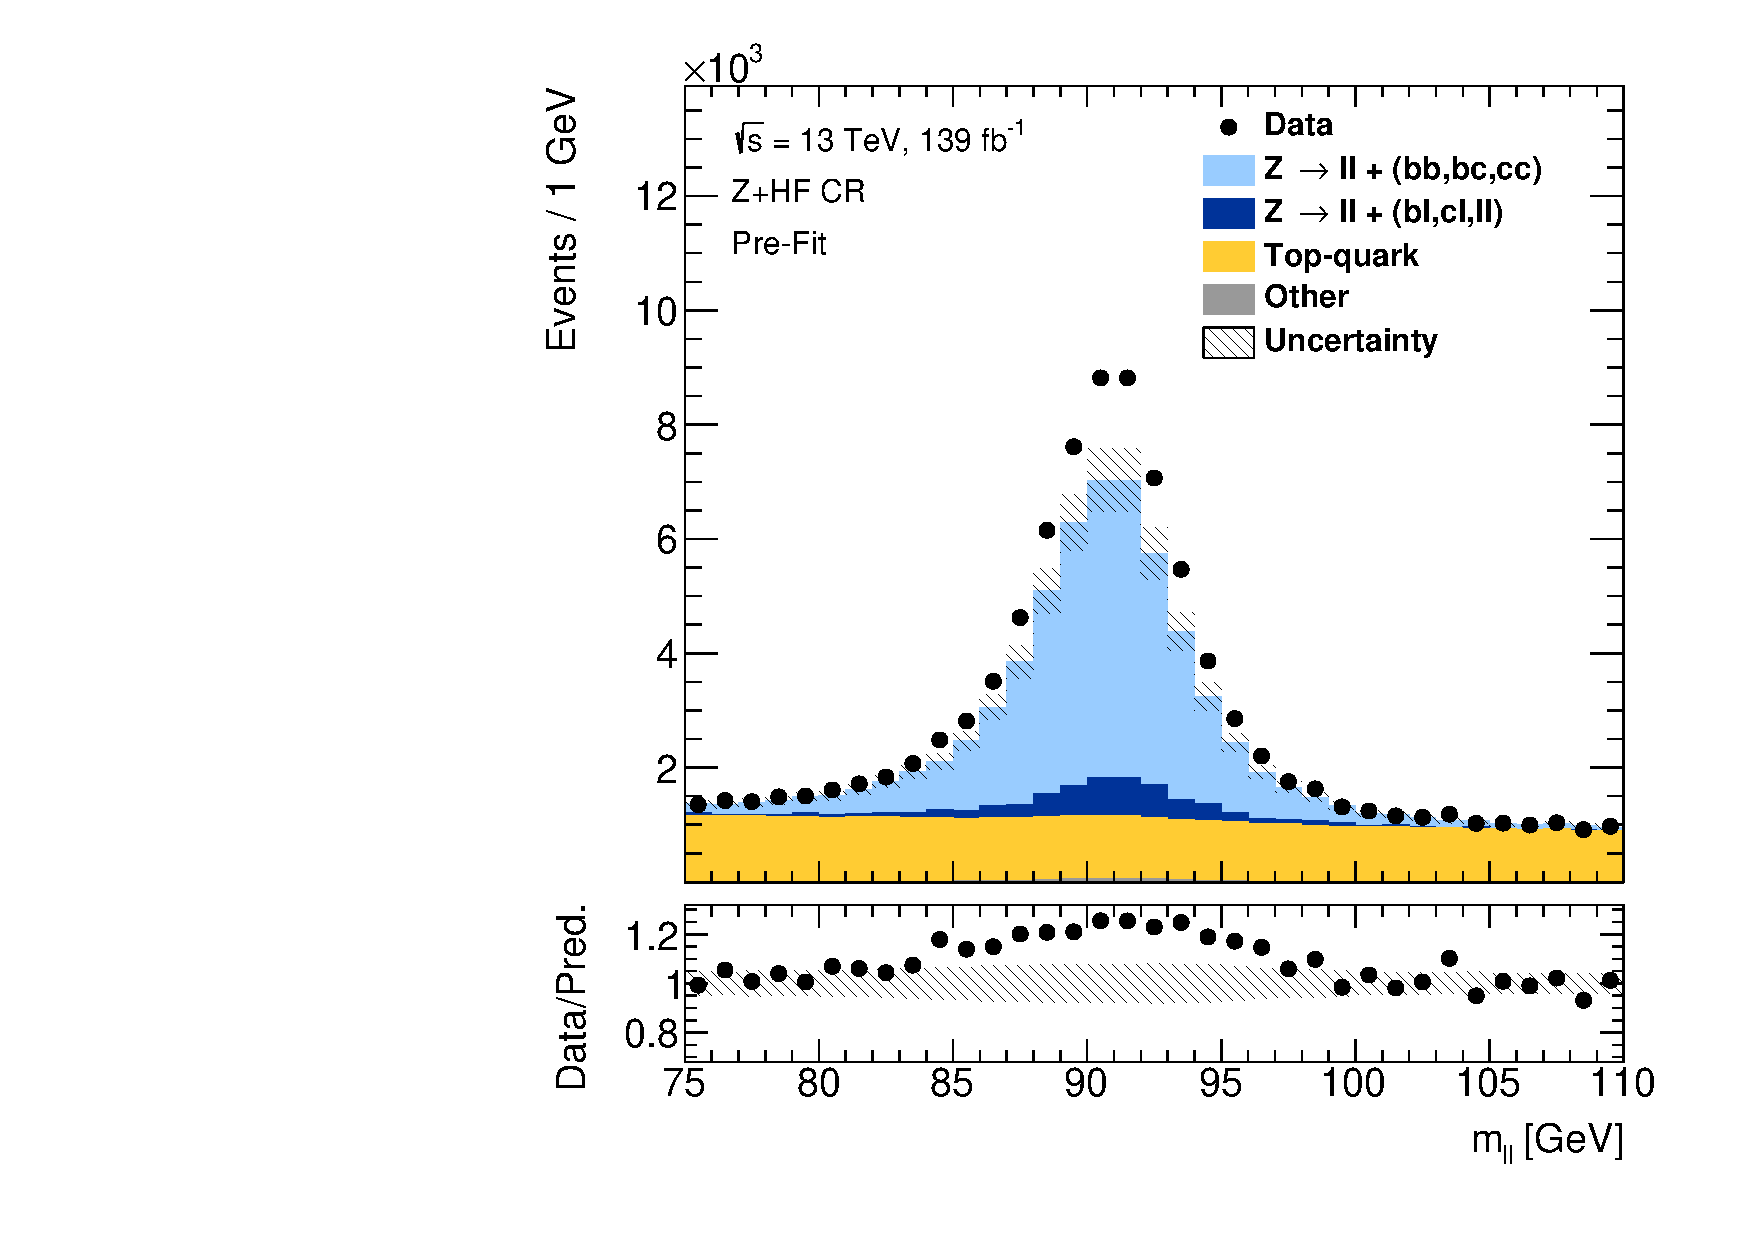
\includegraphics[width=\textwidth]{zhfcr/Region_BMin0_incJet1_Y2015_DZllbbCR_T2_L2_distmLL_J2_Prefit_fixed}
    \subcaption{Pre-fit}
    \label{fig:zcr_mll_prefit}
  \end{subfigure}\hfill%
  \begin{subfigure}{.485\textwidth}
    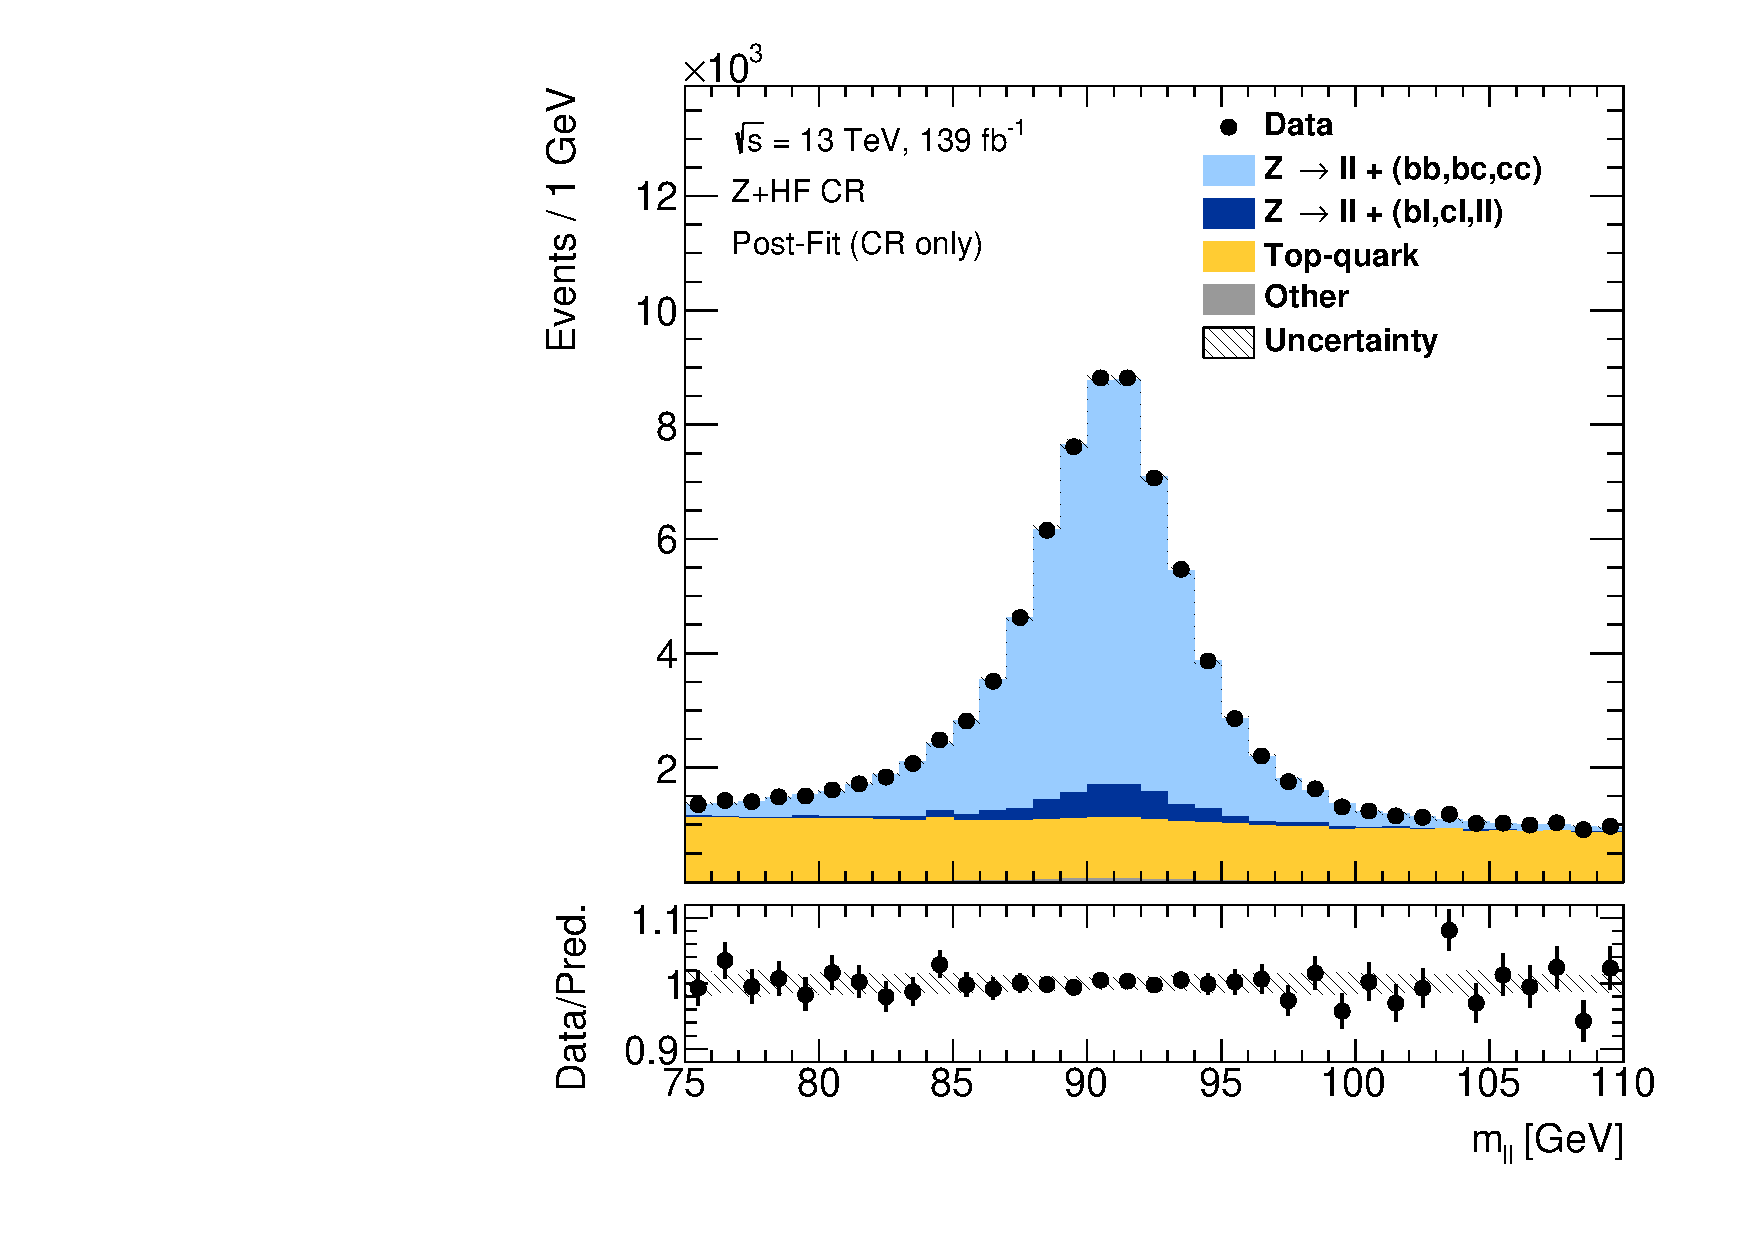
\includegraphics[width=\textwidth]{zhfcr/Region_BMin0_incJet1_Y2015_DZllbbCR_T2_L2_distmLL_J2_GlobalFit_conditionnal_mu0_fixed}
    \subcaption{Post-fit (\ZHF control region only)}
    \label{fig:zcr_mll_postfit}
  \end{subfigure}

  \caption{Distribution of the invariant di-lepton mass for the
    combination of electron- and muon-channel in the Z+HF control
    region before (a) and after (b) the likelihood fit restricted to
    the control region. The contribution of \Zjets is sub-divided into
    cases where both $b$-jet candidates are matched to heavy flavour
    quarks ($b$ or $c$) and cases where at most one candidate is
    matched to heavy flavour quarks at generator-level. Prior to the
    fit the \Zjets background is normalised to cross section
    predictions at NNLO~\cite{Anastasiou:2003ds}. The uncertainty
    includes all statistical and systematic uncertainties.}
\end{figure}

% ATLAS_norm_Zhf    1.3856e+00 +/-  1.19e-01
% ATLAS_norm_ttbar    9.7290e-01 +/-  3.92e-02
% Included in the SR fits: Systematic uncertainties are introduced at a later stage...
The \ZHF control region is included in simultaneous fits of signal and
control regions to provide constraints on the normalisation of the
\ZHF background. Details on systematic uncertainties and the fit model
are discussed
in~\Cref{sec:uncertainties,sec:statistical_analysis}. Restricting the
maximum likelihood fit to the control region yields estimates of the
normalisation factors of \num{1.39 \pm 0.12} and \num{0.97 \pm 0.04}
for \ZHF and \ttbar, respectively. The quoted normalisation factors
include all statistical and systematic
uncertainties. \Cref{tab:zcr_yields} and \Cref{fig:zcr_mll_postfit}
show the event yields and \mll distribution after the fit.



% When performing the likelihood fit in the control region only, the
% estimated normalisation factors are~\num{1.39 \pm 0.12} for the \ZHF
% and~\num{0.97 \pm 0.04} for the \ttbar background. The abundance of
% \ttbar events in the control region provides stringent constraints
% on the normalisation of the \ttbar background in addition to
% constraining the normalisation of the \ZHF background. The post-fit
% event yields and \mll distribution is shown in~\Cref{tab:zcr_yields}
% and~\Cref{fig:zcr_mll_postfit}, respectively.

%%% Local Variables:
%%% mode: latex
%%% TeX-master: "../../phd_thesis"
%%% End:


\subsection{Fake-\tauhadvis Background from \ttbar Production in the \hadhad Channel}%
\label{sec:bkg_hadhad_ttbarfakes}
Top-quark pair production events in which at least one \tauhadvis candidate
originates from a misidentified quark- or gluon-initiated jet are the
second-largest background in the \hadhad channel. A fraction of
\SI{85}{\percent} of events from this background stem from semi-leptonic decay
modes of \ttbar. In these events, the selected \tauhadvis candidates consist of
one true- and one \faketauhadvis. The remaining \SI{15}{\percent} are
\ttbarFakes events with two \faketauhadvis.
% The fraction of \ttbarFakes events with both candidates being \faketauhadvis
% is about \SI{15}{\percent} and thus comparatively small.
The \ttbarFakes background is estimated using simulation after applying
data-driven corrections in the form of \faketauhadvis scale factors (SFs)
measured in a CR enriched in \ttbar events. The SFs correct the \jettotauhadvis
misidentification efficiencies predicted by simulation, which are not centrally
calibrated by the ATLAS collaboration due to their process dependency.

Before proceeding with the description of the method, differences between
\faketauhadvis backgrounds from \ttbar and multi-jet are highlighted that
motivate the use of different background estimation techniques:
\begin{itemize}

\item The majority of \ttbarFakes background events consist of only one
  \faketauhadvis, while in multi-jet events both candidates are \faketauhadvis.

\item The probability that a quark- or gluon-initiated jet reconstructed as
  \tauhadvis passes \tauid, also called the \emph{fake rate}, depends on the
  type of parton that initiated the jet. In \ttbar events, \faketauhadvis
  predominately originate from quarks produced in decays of $W$~bosons, which
  have larger fake rates than gluon-initiated jets. As a result, \faketauhadvis
  background estimation is inherently process dependent.

\item In the \hadhad channel, no suitable \ttbarFakes CR can be defined that
  separates \faketauhadvis backgrounds from \ttbar and multi-jet while
  maintaining sufficient statistical precision for background estimation. This
  necessitates defining a CR in $\ell + \tauhadvis$ ($\ell = e, \mu$) final
  states in which the multi-jet contribution can be neglected.

\end{itemize}
The main disadvantage of separately estimating the \faketauhadvis background
from \ttbar and multi-jet is the inflation of systematic uncertainties on the
estimate of the total \faketauhadvis background compared to a combined
approach.\footnote{An example of a combined approach is the combined fake factor
  method employed in the \lephad channel. This method is summarised
  in~\Cref{sec:bkg_lephad_combined_ff}.}  However, these inflated uncertainties
have little effect on the signal sensitivity for two reasons: First, the
targeted signal processes have distinct kinematic properties that differentiate
them from \faketauhadvis backgrounds. Second, the search is limited by
statistical uncertainties as opposed to systematic ones.


\subsubsection{Control Region Definition}

The CR for the SF measurement (SF-CR) targets final states with an electron or
muon and a \tauhadvis candidate. The region definition is based on the
selections applied in the \lephad channels, where a similar CR is used for
\faketauhadvis background estimation. Minor changes are applied to its
definition to ensure consistency with the SR selection of the \hadhad
channel. The most important selection criteria and differences are briefly
summarised:
\begin{itemize}

\item The \tauhadvis selection is adapted to follow the selection of the \hadhad
  channel more closely by selecting candidates with $\pT > \SI{25}{\GeV}$ and
  $|\eta| < \num{2.5}$ (instead of $\pT > \SI{20}{\GeV}$ and
  $|\eta| < \num{2.3}$ in the \lephad channels).

\item All events are required to have exactly one \tauhadvis candidate passing
  \tauid, exactly one electron or muon passing their respective isolation and
  identification criteria, and exactly two \btagged jets. In addition, only
  events passing the SLT selection are considered.

\item The electron/muon and the \tauhadvis candidate are required to be
  reconstructed with electric charges of opposite sign.
  % This requirement ensures that the charge correlations between light lepton
  % and \faketauhadvis from semi-leptonic decays of \ttbar are similar to the
  % correlation between \tauhadvis candidates from \ttbarFakes in the \hadhad SR
  % for cases where only one candidate is a \faketauhadvis. The effect of charge
  % correlation on \ttbarFakes estimation was previously studied in
  % Ref.~\cite{bokan}.

\item Orthogonality between the SF-CR and the SR of the \lephad SLT channel is
  ensured by requiring $\mBB > \SI{150}{\GeV}$.

\end{itemize}

% \footnote{Leptons $\ell$ and true \tauhadvis are have high
% probability to be reconstructed with the correct electric charge in
% the SF-CR. In \ttbar the \faketauhadvis candidate is more likely to
% have opposite-sign electric charge . As a result, in the same-sign
% region the quark/gluon composition of jets is likely different which
% also affects the fake rates.}.

The dominant process populating the SF-CR is \ttbar production, which is
selected with a purity of \SI{94}{\percent}. About \SI{66}{\percent} of SF-CR
events are from di-leptonic decay modes of \ttbar that yield an electron/muon
and a \tauhadvis in the final state. The production of \ttbar events with
\tauhadvis candidates originating from quark- or gluon-initiated jets, which is
the process of interest for this measurement, constitutes \SI{28}{\percent} of
selected events. Minor backgrounds in this region are single-top-quark
(\SI{4}{\percent}) and $\Vjets$ (\SI{2}{\percent}) production. The \multijet
background is assumed to be negligible. The distribution of transverse momenta
and pseudorapidity of \tauhadvis candidates in the SF-CR prior to the fit is
shown in~\Cref{fig:ttbarSF_prefit_pt}.

\begin{figure}[htbp]
  \centering

  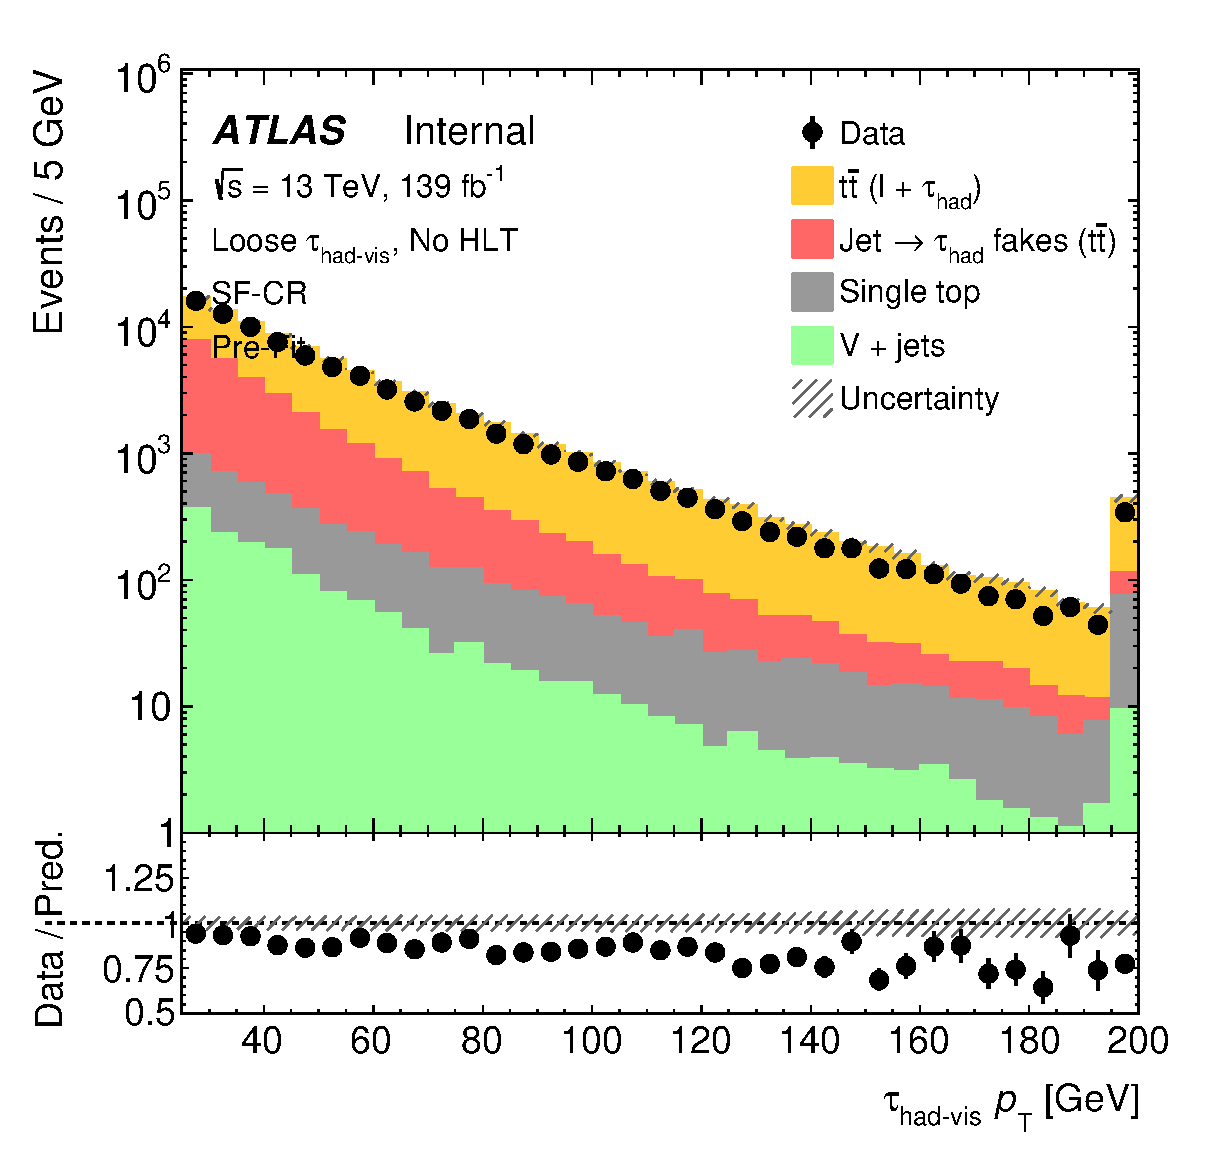
\includegraphics[width=0.49\textwidth]{ttbarSF/prefit_sfcr/PTVR}%
  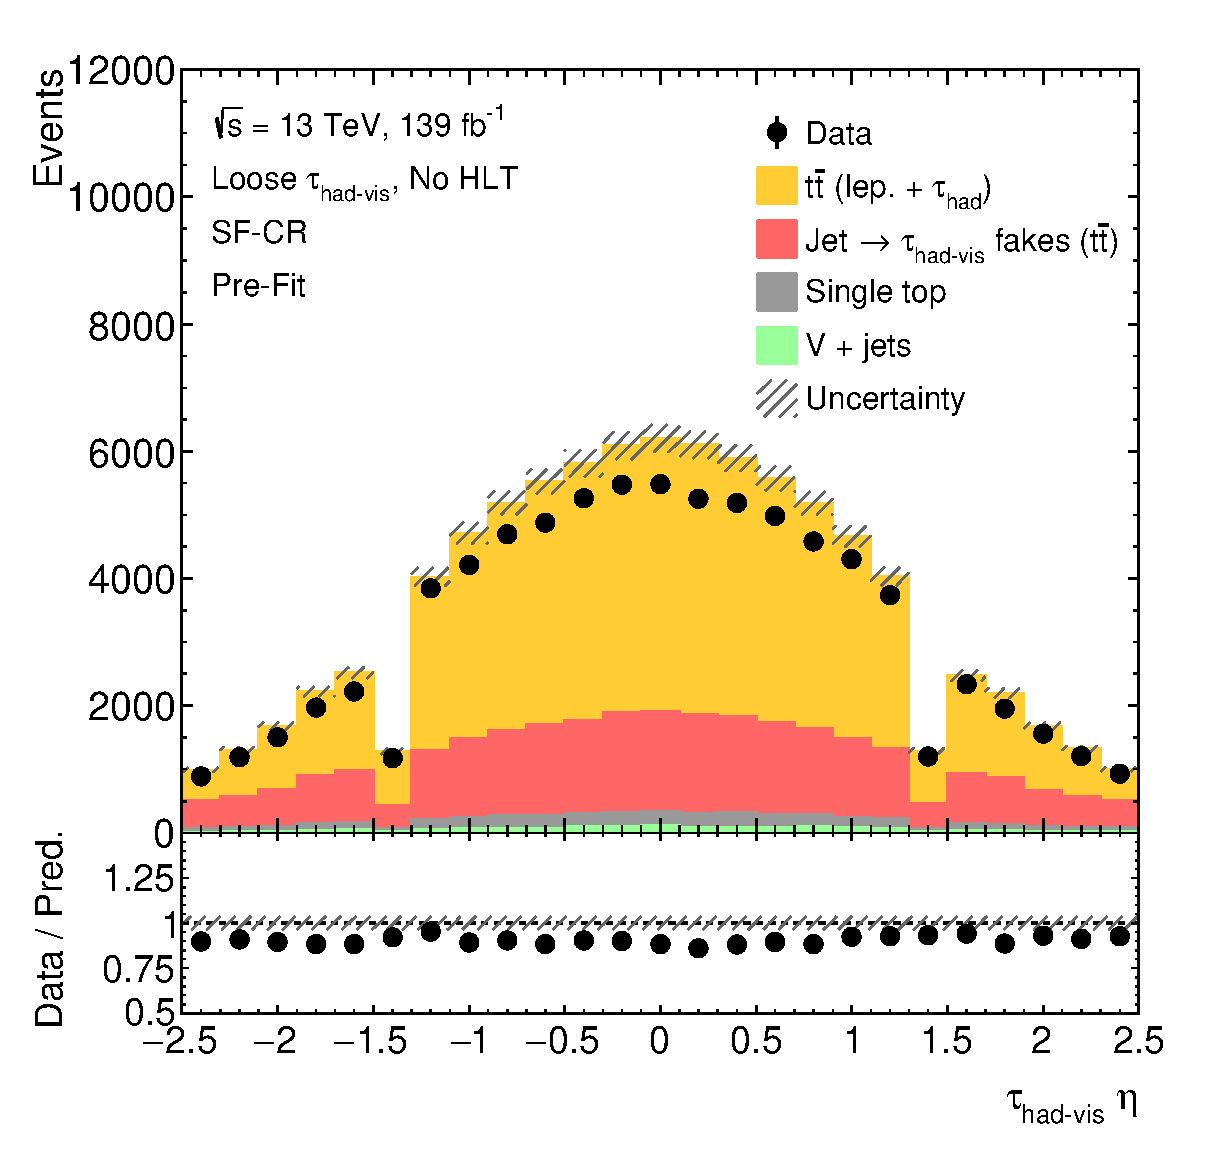
\includegraphics[width=0.49\textwidth]{ttbarSF/prefit_sfcr/ETAVR}

  \caption[Distribution of \tauhadvis \pT and $\eta$ in the SF-CR.]{Distribution
    of \tauhadvis \pT and $\eta$ in the SF-CR prior to the fit. Events with
    \tauhadvis candidate \pT larger than \SI{200}{\GeV} are included in the last
    bin. All statistical and systematic uncertainties are included.}%
  \label{fig:ttbarSF_prefit_pt}
\end{figure}

\Jettotauhadvis misidentification efficiencies depend on the identification
requirements applied to \tauhadvis candidates. In this search, such requirements
are imposed on \tauhadvis candidates at trigger-level and during offline event
reconstruction. This two-stage selection of \tauhadvis candidates is taken into
account by measuring separate sets of SFs for every relevant combination of
\tauid requirements. One set of SFs is measured for \faketauhadvis after offline
\tauid but without requirements at trigger-level.
% These SFs are required for STT events in the \hadhad channel in cases where
% the \faketauhadvis was not the candidate causing the trigger to select the
% event.
Three sets of SFs are measured to account for identification requirements
applied at trigger-level and during offline event reconstruction.
% chains used in the \hadhad channel (cf.~\Cref{sec:hadhad_trigger_selection})
% which are applied in addition to offline \tauid.

The measurement of SFs without requirements at trigger-level can proceed using
events in the SF-CR without additional selections. For measurements of SFs that
include trigger-level identification requirements, the selections applied by
\tauhadvis-triggers need to be emulated. This is achieved by requiring that
events in the SF-CR are also selected by appropriately chosen single-\tauhadvis
triggers. In addition, the reconstructed \tauhadvis candidate has to be
geometrically matched ($\Delta R < 0.2$) to a \tauhadvis candidate at the HLT
that fulfilled the trigger criteria. The SF measurement is performed for three
different \tauhadvis-triggers (cf.\ \Cref{sec:hadhad_trigger_selection}):
\begin{itemize}
\item \verb|HLT_tau25_medium1_tracktwo| %(\SI{139}{\ifb})
\item \verb|HLT_tau25_medium1_tracktwoEF| %(\SI{58}{\ifb})
\item \verb|HLT_tau25_medium1_tracktwoEF or HLT_tau25_mediumRNN_tracktwoMVA|
  % (\SI{37}{\ifb})
\end{itemize}
During Run~2 of the LHC, these triggers had to be prescaled to limit their
trigger rates.\footnote{A trigger with a prescale value of $n$ accepts events
  satisfying the trigger conditions with a probability of $1 / n$
  \cite{TRIG-2019-04}.} However, events passing the SF-CR selection were already
recorded using unprescaled single-lepton triggers. This allows single-\tauhadvis
to be re-run during offline event reconstruction without application of a
prescale.
% This allows to re-run the single-\tauhadvis triggers used in this measurement
% during offline event reconstruction without application of a prescale.
The \verb|HLT_tau25_medium1_tracktwo| trigger chain was active for the entirety
of Run~2 of the LHC. Trigger decisions for the
\verb|HLT_tau25_medium1_tracktwoEF| and \verb|HLT_tau25_mediumRNN_tracktwoMVA|
trigger chains are only available for partial datasets with integrated
luminosities of \SI{58}{\ifb} and \SI{37}{\ifb}, respectively.


\subsubsection{Scale Factor Measurement}

The \jettotauhadvis misidentification efficiencies strongly depend on the
charged-particle multiplicity and transverse momentum of reconstructed
\tauhadvis candidates. This might also be reflected in corrections of the
\jettotauhadvis misidentification efficiencies in simulation. Therefore, the SF
measurement is performed in regions of \Ntracks and \pT of the \tauhadvis
candidate given by:
\begin{itemize}

\item $\Ntracks = 1$ and $\pT / \si{\GeV}$: $[25, 30)$, $[30, 35)$, $[35, 40)$,
  $[40, 45)$, $[45, 55)$, $[55, 70)$, $[70, \infty)$.

\item $\Ntracks = 3$ and $\pT / \si{\GeV}$: $[25, 30)$, $[30, 40)$, $[40, 50)$,
  $[50, 70)$, $[70, \infty)$.

\end{itemize}
These regions are chosen such that their size allows for a determination of the
corrections with limited impact of statistical uncertainties while extracting
potential \pT-dependencies of the correction factors. In cases where events are
required to pass single-\tauhadvis triggers, the \pT intervals from 25 to
\SI{30}{\GeV} are omitted to ensure that the \tauhadvis-triggers operate in a
regime where they are well-calibrated. This is analogous to the selections
applied in the SR of the \hadhad channel. Two examples of event yields in the
regions entering the SF measurement are shown
in~\Cref{fig:ttbarsf_region_summary_prefit}.

\begin{figure}[htbp]
  \centering

  \begin{subfigure}[t]{.48\textwidth}
    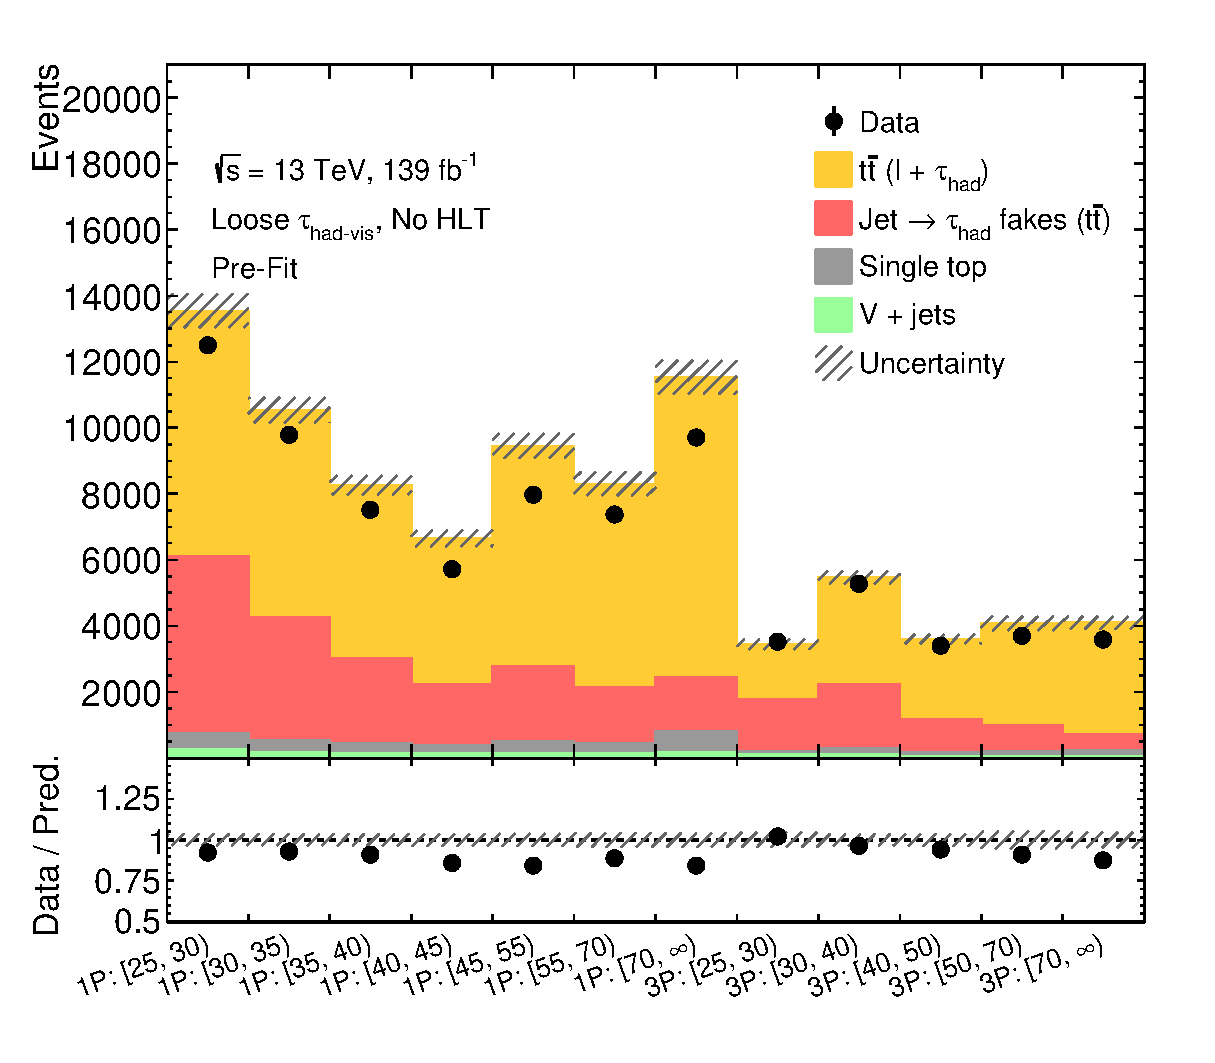
\includegraphics[width=\textwidth]{ttbarSF/Summary_offl}

    \caption{Events without trigger-level \tauid requirements.}
  \end{subfigure}\hfill%
  \begin{subfigure}[t]{.48\textwidth}
    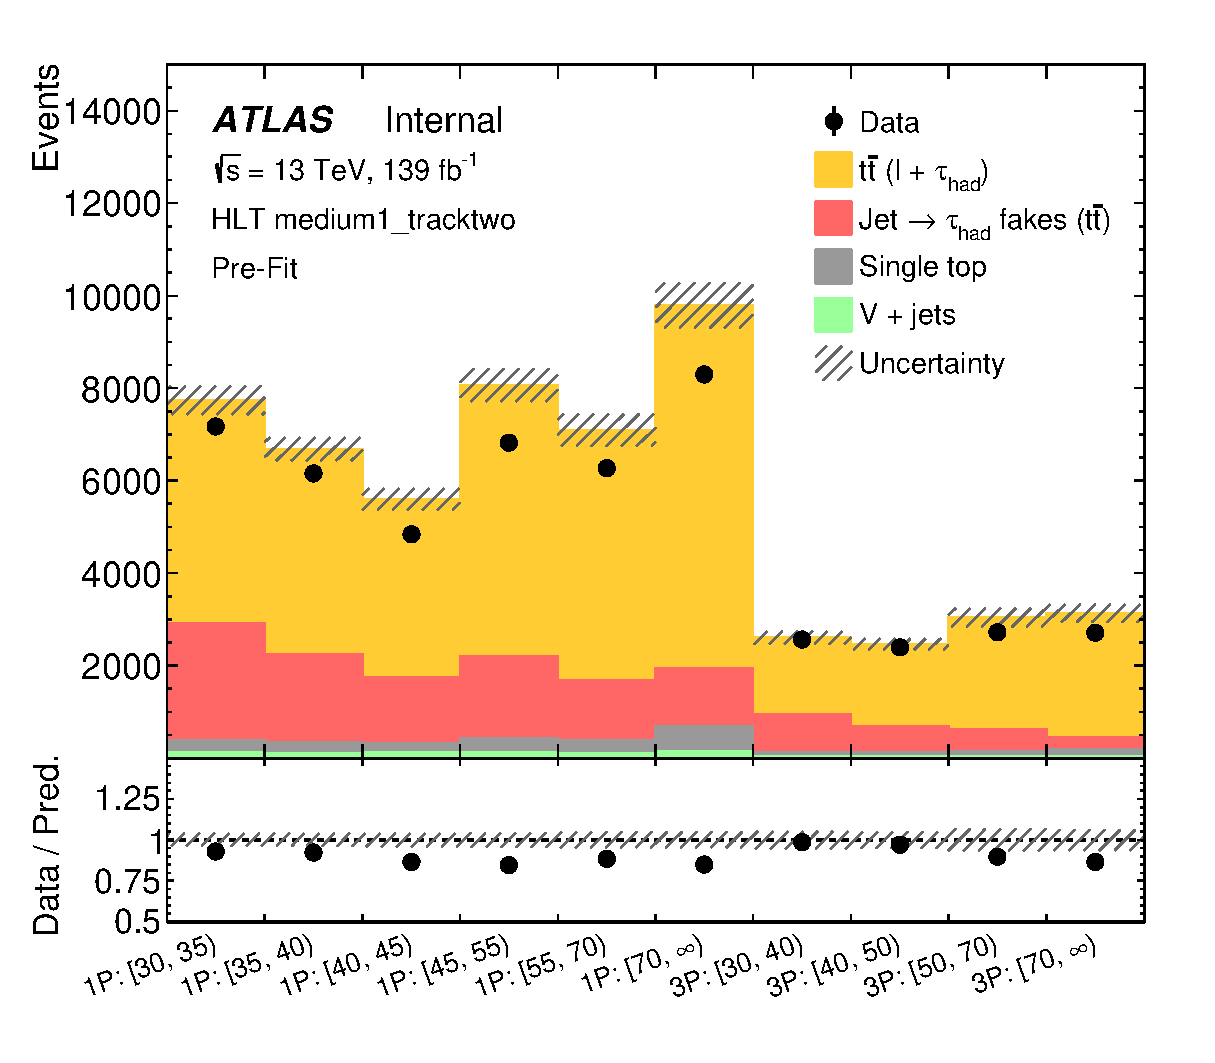
\includegraphics[width=\textwidth]{ttbarSF/Summary_tau25}

    \caption{Events passing \tauhadvis trigger-matching and the
      \texttt{HLT\_tau25\_medium1\_tracktwo} trigger.}
  \end{subfigure}

  \caption[Expected and observed event yields in regions of \tauhadvis candidate
  \Ntracks and \pT in the SF-CR.]{Expected and observed event yields in regions
    of \tauhadvis candidate \Ntracks and \pT in the SF-CR. The bins are labelled
    as ``1P'' and ``3P'' for $\Ntracks = 1$ and $\Ntracks = 3$, respectively,
    and the \pT intervals are given in units of \si{\GeV}. The background model
    is shown prior to the fit.}%
  \label{fig:ttbarsf_region_summary_prefit}
\end{figure}

A discriminant is required to distinguish between \ttbar with and without
\faketauhadvis since only the former is sensitive to \jettotauhadvis
misidentification efficiencies. The transverse mass of the electron/muon and
\pTmissAbs is used for this purpose, which is defined as
\begin{align*}
  \mTW = \sqrt{2 | \myvec{p}_{\text{T}}^{\ell} | | \pTmiss | \left( 1 - \cos \Delta\phi \right)} \,\text{,}
\end{align*}
where $\Delta \phi$ is the angle between the lepton transverse momentum,
$\myvec{p}_{\text{T}}^{\ell}$, and the missing transverse momentum, \pTmiss. The
\mTW discriminant targets the differences between di- and semi-leptonic decay
modes of \ttbar that are the primary sources of events with true- and
\faketauhadvis, respectively. The differences are illustrated
in~\Cref{fig:ttbarsf_mtw_pdf} with di-leptonic decay modes of \ttbar showing a
heavy tail towards large \mTW due to the presence of additional neutrinos, while
semi-leptonic decay modes have a pronounced peak close to the mass of the
$W$~boson.


\begin{figure}[htbp]
  \centering

  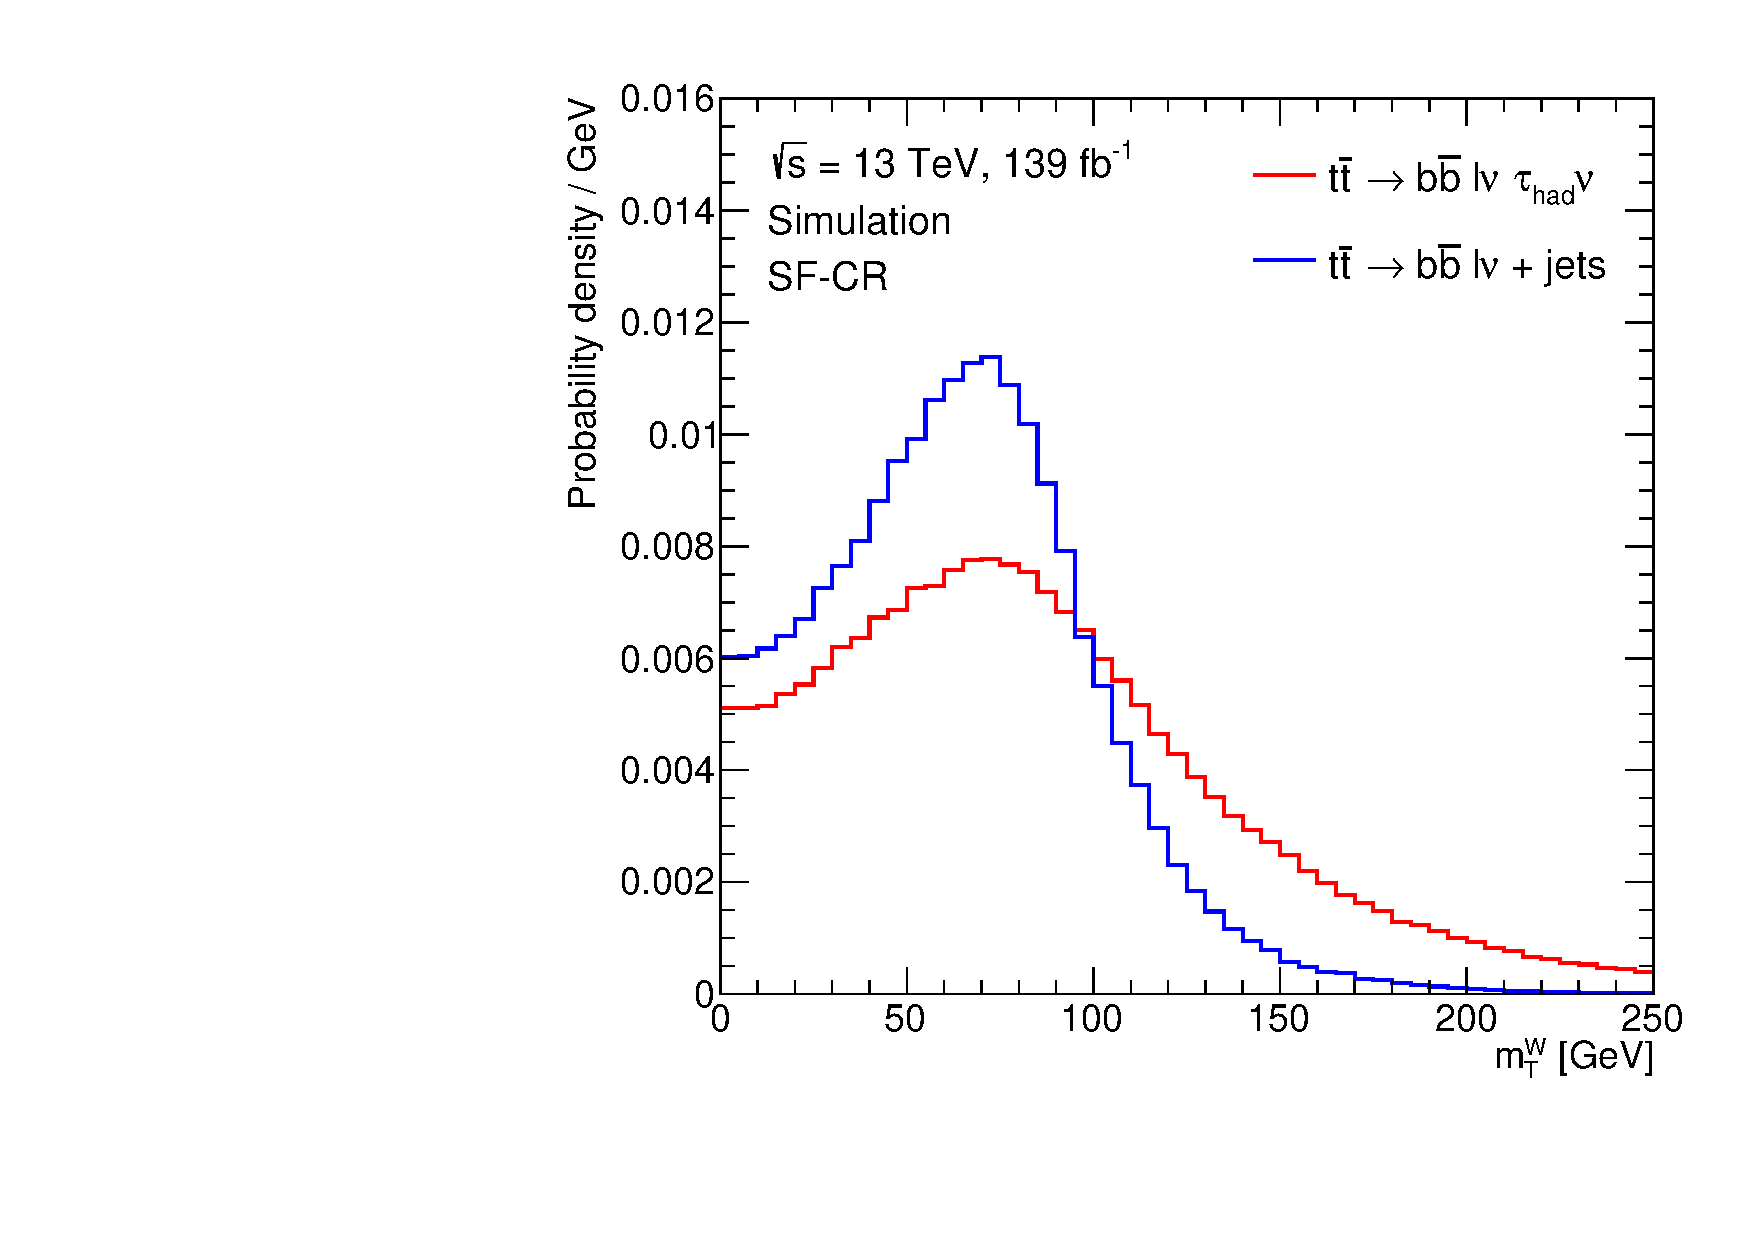
\includegraphics[width=0.45\textwidth, trim=0.5cm 1.5cm 0.3cm 0.3cm,
  clip]{ttbarSF/mtw_pdf}

  \caption[Distribution of the transverse mass of the lepton and \pTmiss for
  simulated \ttbar events in the SF-CR.]{Distribution of the transverse mass of
    the lepton and \pTmiss for simulated \ttbar events in the SF-CR. The
    distributions are inclusive in \pT and \Ntracks of the \tauhadvis
    candidate.}%
  \label{fig:ttbarsf_mtw_pdf}
\end{figure}

The \faketauhadvis SFs are measured using a simultaneous likelihood fit of the
binned \mTW distributions in all regions of \tauhadvis candidate \pT and
\Ntracks. The fit model is constructed using simulated \ttbar, single-top, and
\Vjets events. The sample of \ttbar events is split by whether the reconstructed
\tauhadvis candidate is a \faketauhadvis or not. The overall normalisation of
the \ttbar background, irrespective of whether events contain a \faketauhadvis,
is free to vary in the model.  In every region of \tauhadvis candidate
\Ntracks and \pT, an unconstrained SF is introduced that changes the
normalisation of the \ttbarFakes background in this region. These \faketauhadvis
SFs are considered as the POIs of the measurement.

The pre-fit expectation of the model in two exemplary regions is shown
in~\Cref{fig:ttbarsf_mtw_examples_prefit} for SF-CR events passing the
\verb|HLT_tau25_medium1_tracktwo| trigger and trigger-matching. The binning of
the \mTW discriminants is the same in all \tauhadvis candidate \pT and \Ntracks
regions.

\begin{figure}[htbp]
  \centering

  \begin{subfigure}{.48\textwidth}
    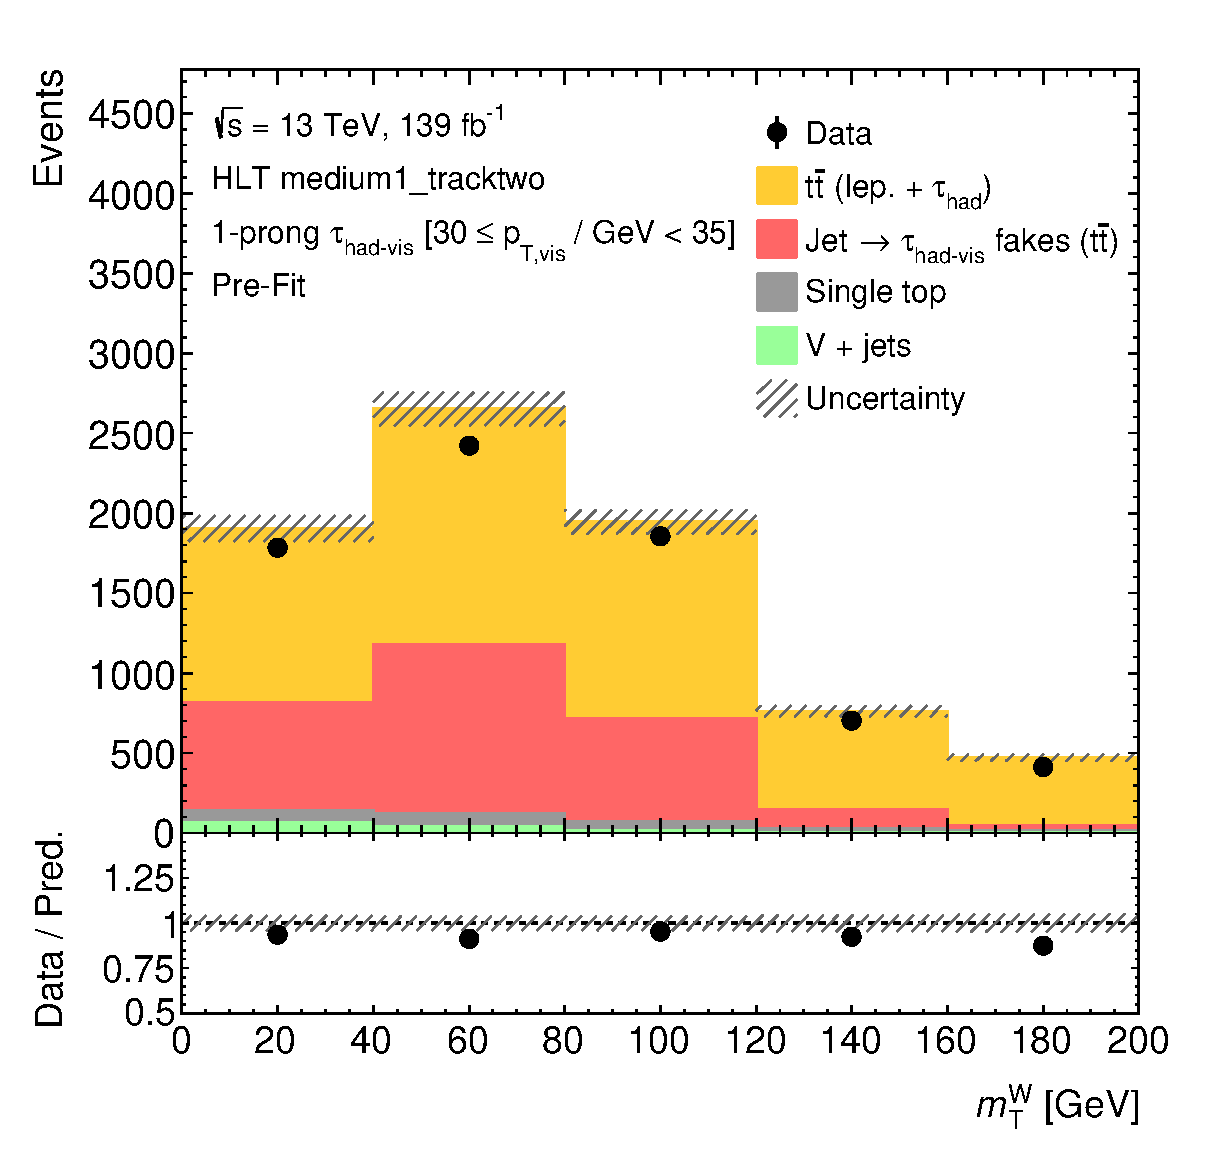
\includegraphics[width=\textwidth]{ttbarSF/tau25/TauPt3035_1P}
    \caption{$\Ntracks = 1$ and $\SI{30}{\GeV} \leq \pT < \SI{35}{\GeV}$.}
  \end{subfigure}\hfill%
  \begin{subfigure}{.48\textwidth}
    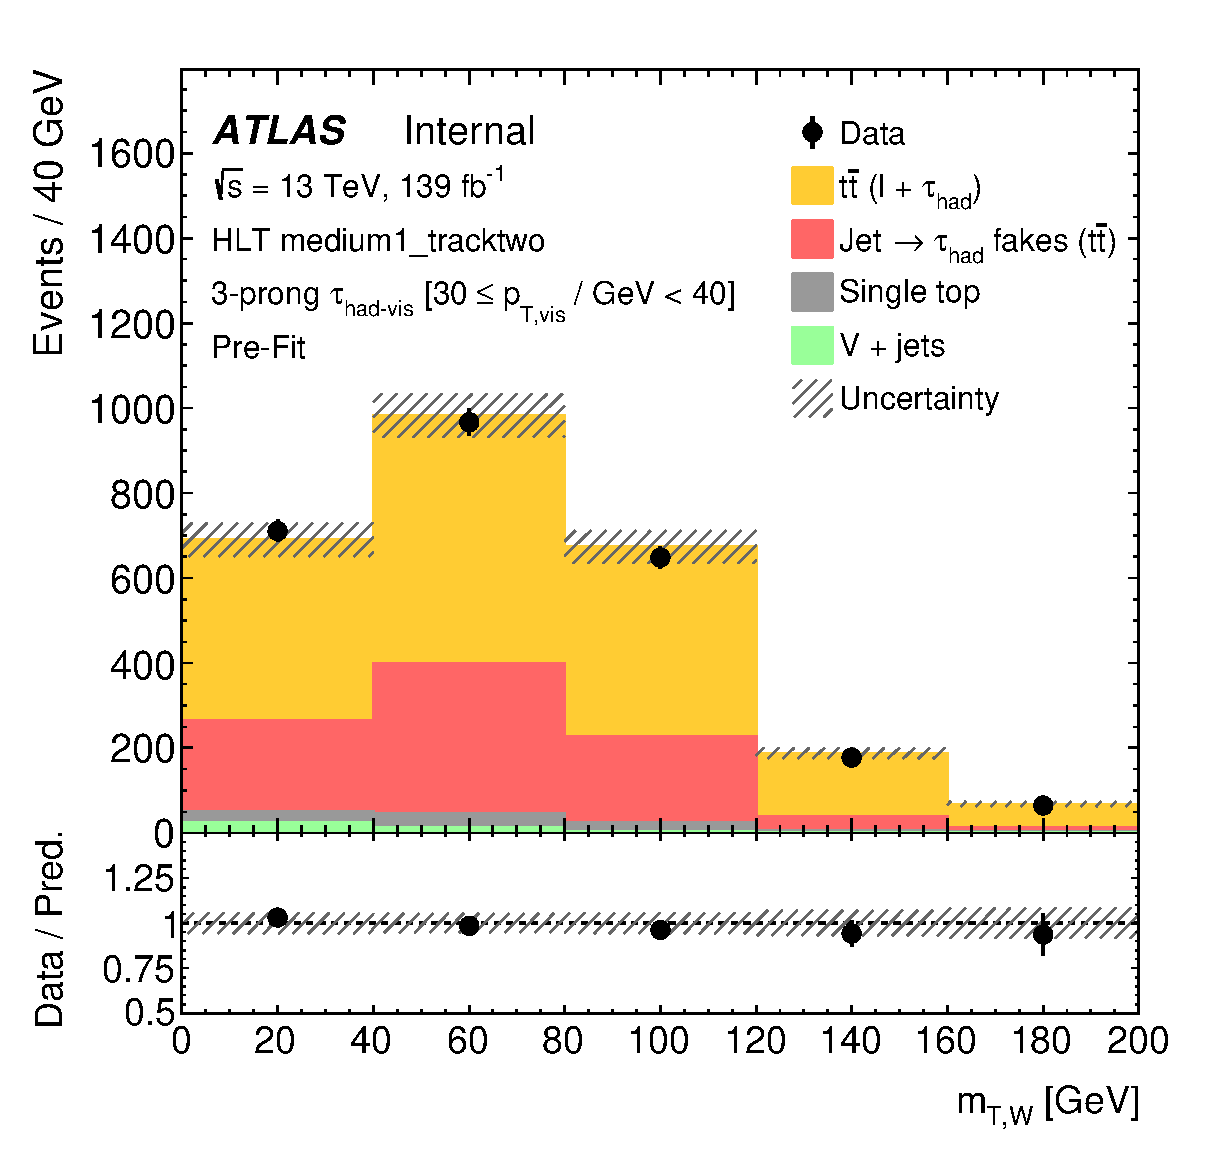
\includegraphics[width=\textwidth]{ttbarSF/tau25/TauPt3040_3P}
    \caption{$\Ntracks = 3$ and $\SI{30}{\GeV} \leq \pT < \SI{40}{\GeV}$.}
  \end{subfigure}

  \caption[Pre-fit \mTW distribution in two exemplary regions of the SF
  measurement.]{Pre-fit \mTW distribution in two exemplary \tauhadvis candidate
    \Ntracks and \pT regions of the SF measurement after requiring events to
    pass the \texttt{HLT\_tau25\_medium1\_tracktwo} trigger and
    trigger-matching. Events with $\mTW > \SI{200}{\GeV}$ are included in the
    last bin of the histograms.}%
  \label{fig:ttbarsf_mtw_examples_prefit}
\end{figure}


\subsubsection{Uncertainties in the Scale Factor Measurement}

Several experimental and theoretical uncertainties are considered in the SF
measurement. In general, these uncertainties can affect the normalisation and
shape of the expected \mTW distribution for a given process in all regions
entering the fit. The uncertainties included in the SF measurement and their
treatment closely follows the approach taken in
\Cref{sec:uncertainties,sec:statistical_analysis} to interpret the results of
the search for Higgs boson pair production. Therefore, the uncertainties
included in the SF measurement are only briefly summarised.

Experimental uncertainties affecting the reconstruction and selection
efficiencies of electrons, muons, \tauhadvis, and jets are accounted for in the
SF measurement, including uncertainties on the efficiencies of
$b$-tagging. Uncertainties on the reconstructed \pTmissAbs are propagated to the
\mTW distributions in all regions. Trigger efficiency uncertainties are
considered for single-lepton and single-\tauhadvis
triggers.\footnote{Uncertainties on single-\tauhadvis trigger efficiencies are
  only considered for SF measurements taking into account trigger-level \tauid
  requirements.}  Uncertainties on the re-weighting of the pile-up conditions in
simulation and the integrated luminosity used to normalise simulated event
samples are included in the measurement as well. Lastly, statistical
uncertainties from the finite size of the simulation samples are included
according to the simplified Barlow--Beeston method~\cite{barlow1993,conway2011}.

Theory uncertainties on the modelling of \ttbar production using simulation are
derived for this measurement according to prescriptions developed by the ATLAS
collaboration, which are summarised in \Cref{app:top_uncertainties}. An
uncertainty on the simulation of the hard interaction and matching to the parton
shower is derived by comparison with an alternative matrix element generator and
matching scheme. Uncertainties on the modelling of the parton shower,
hadronisation, and underlying event are determined by comparison with an
alternative parton shower program. The effect of missing higher orders in the
truncated perturbative expansion in \alphas is probed by performing variations
of renormalisation and factorisation scales. Finally, uncertainties on the
modelling of additional emissions are derived by performing variations of the
simulated initial- and final-state radiation. Modelling uncertainties are
derived separately for \ttbar events with and without \faketauhadvis, but are
regarded as correlated in the fit model if they originate from the same
source. Effects of the \ttbar modelling uncertainties on the shape of the \mTW
discriminants and the expected number of events in different \tauhadvis
candidate \Ntracks and \pT regions are considered in the fit model.

Reduced sets of theory uncertainties are considered for minor backgrounds in the
SF measurement. Uncertainties on the cross sections of single-top and \Vjets
production are included in the model. Due to the known normalisation discrepancy
of \Vjets production in the presence of jets originating from heavy flavour
quarks, an additional normalisation uncertainty of \SI{30}{\percent} is assigned
to the \Vjets background.


\subsubsection{Results of the Scale Factor Measurement}

The measured \faketauhadvis SFs are shown in \Cref{fig:ttbarSF_postfit_SF}.
% for all relevant \tauid criteria.
The size of the corrections described by the SFs can reach up to
\SI{55}{\percent} for \faketauhadvis of high \pT where simulation overestimates
the contribution of \faketauhadvis in \ttbar. SFs for \faketauhadvis
reconstructed as 1-prong (3-prong) candidates with $\pT < \SI{70}{\GeV}$ are
within \SI{20}{\percent} (\SI{40}{\percent}) of unity. Only small differences
are observed between SFs measured for different \tauid requirements at
trigger-level as is shown
in~\Cref{fig:ttbarSF_postfit_SF_c,fig:ttbarSF_postfit_SF_d}.

\begin{figure}[htbp]
  \centering

  \begin{subfigure}[t]{.495\textwidth}
    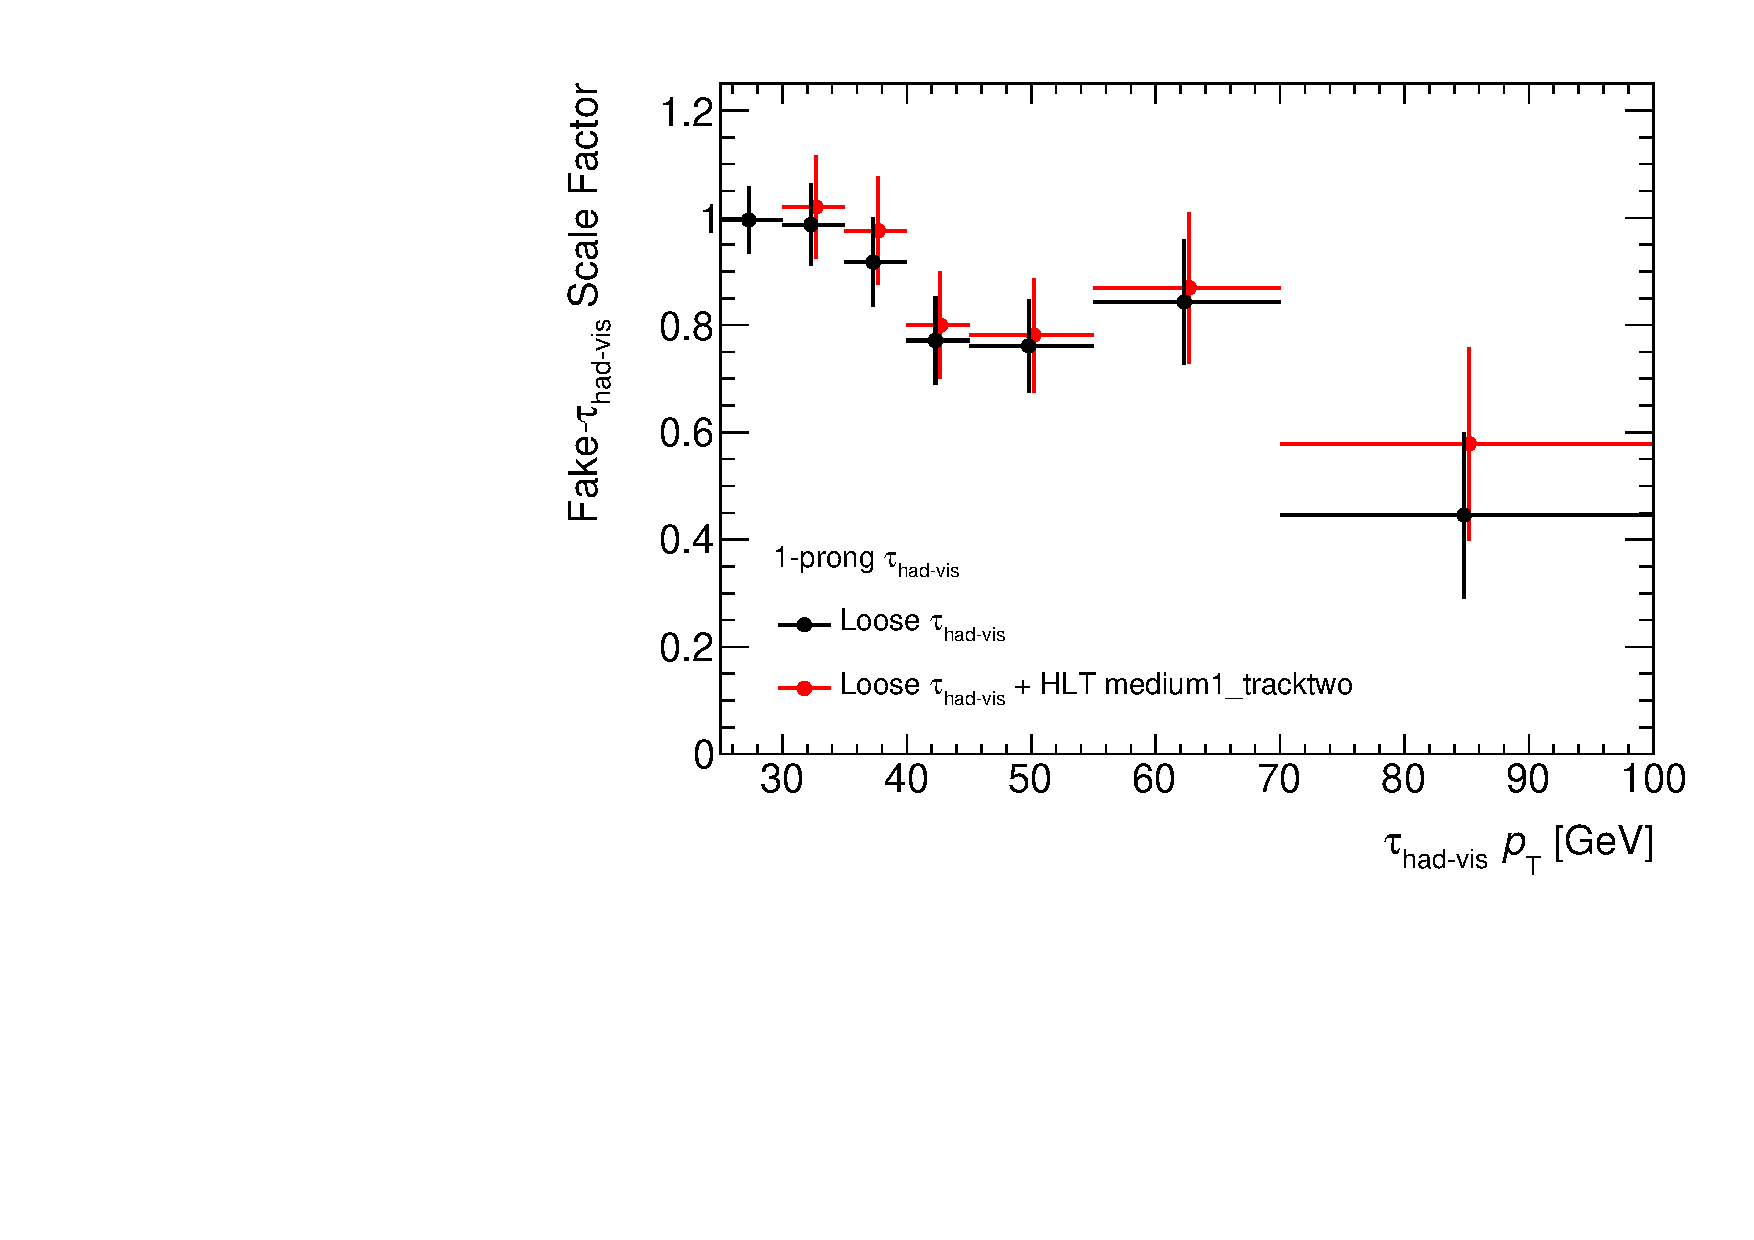
\includegraphics[width=\textwidth]{ttbarSF/ttbarSF_offl_tau25_1p}
    \caption{}
    \label{fig:ttbarSF_postfit_SF_a}
  \end{subfigure}\hfill%
  \begin{subfigure}[t]{.495\textwidth}
    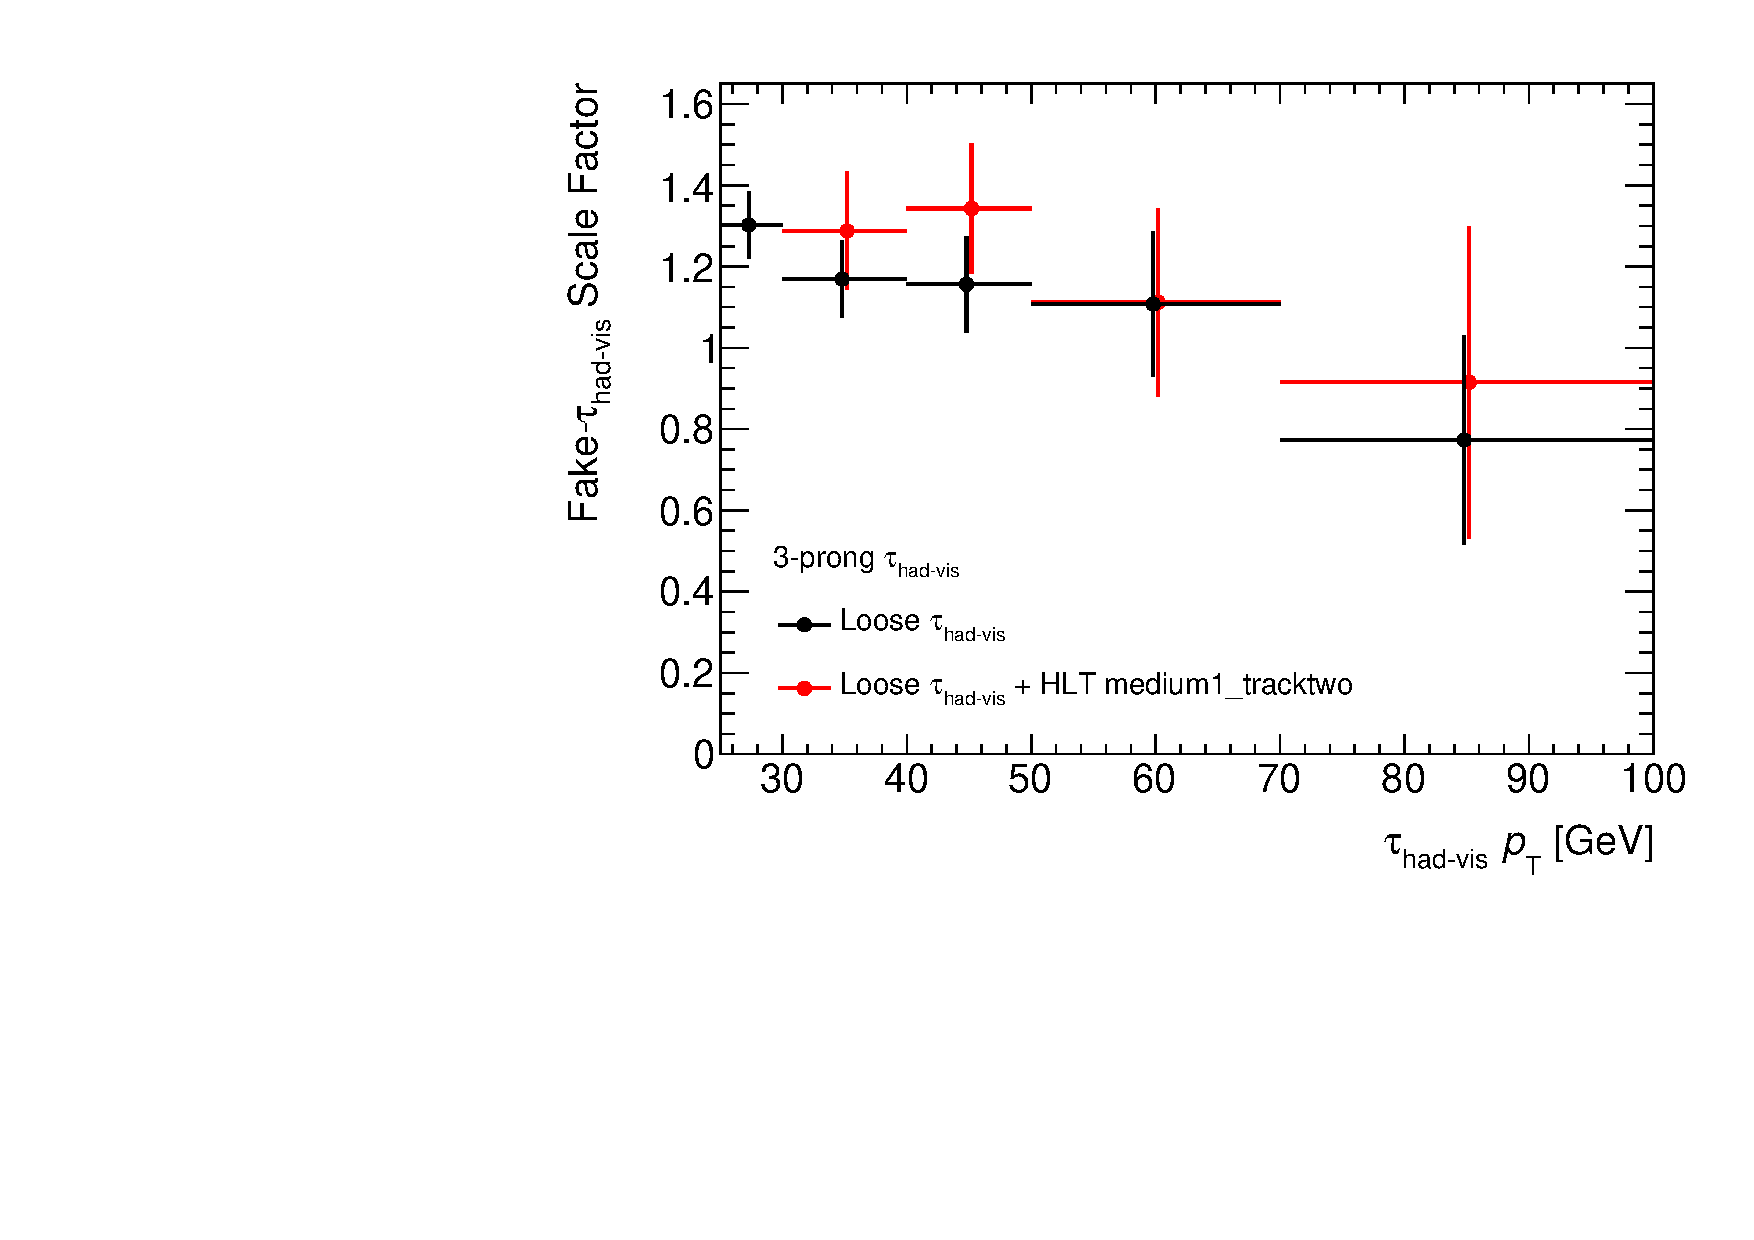
\includegraphics[width=\textwidth]{ttbarSF/ttbarSF_offl_tau25_3p}
    \caption{}
    \label{fig:ttbarSF_postfit_SF_b}
  \end{subfigure}

  \begin{subfigure}[t]{.495\textwidth}
    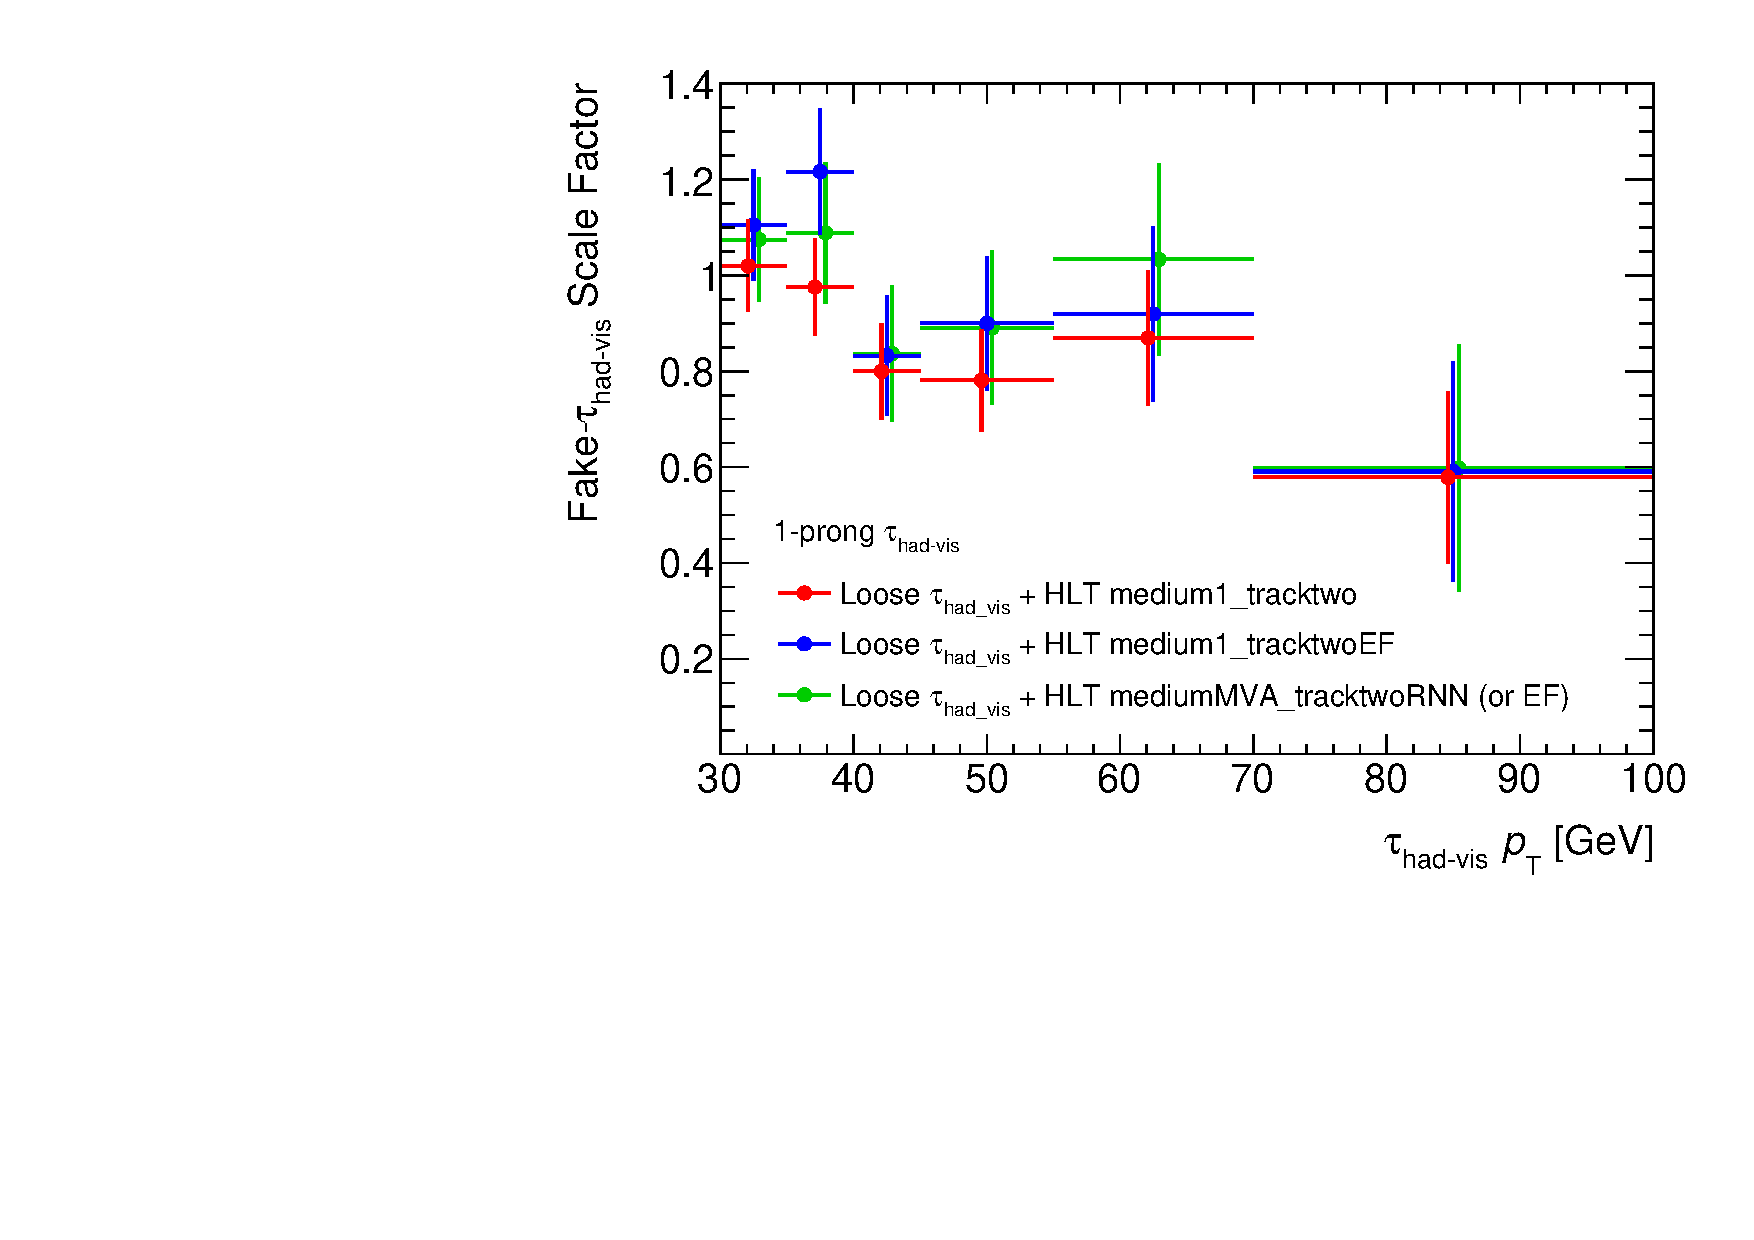
\includegraphics[width=\textwidth]{ttbarSF/ttbarSF_tau25_1p}
    \caption{}
    \label{fig:ttbarSF_postfit_SF_c}
  \end{subfigure}\hfill%
  \begin{subfigure}[t]{.495\textwidth}
    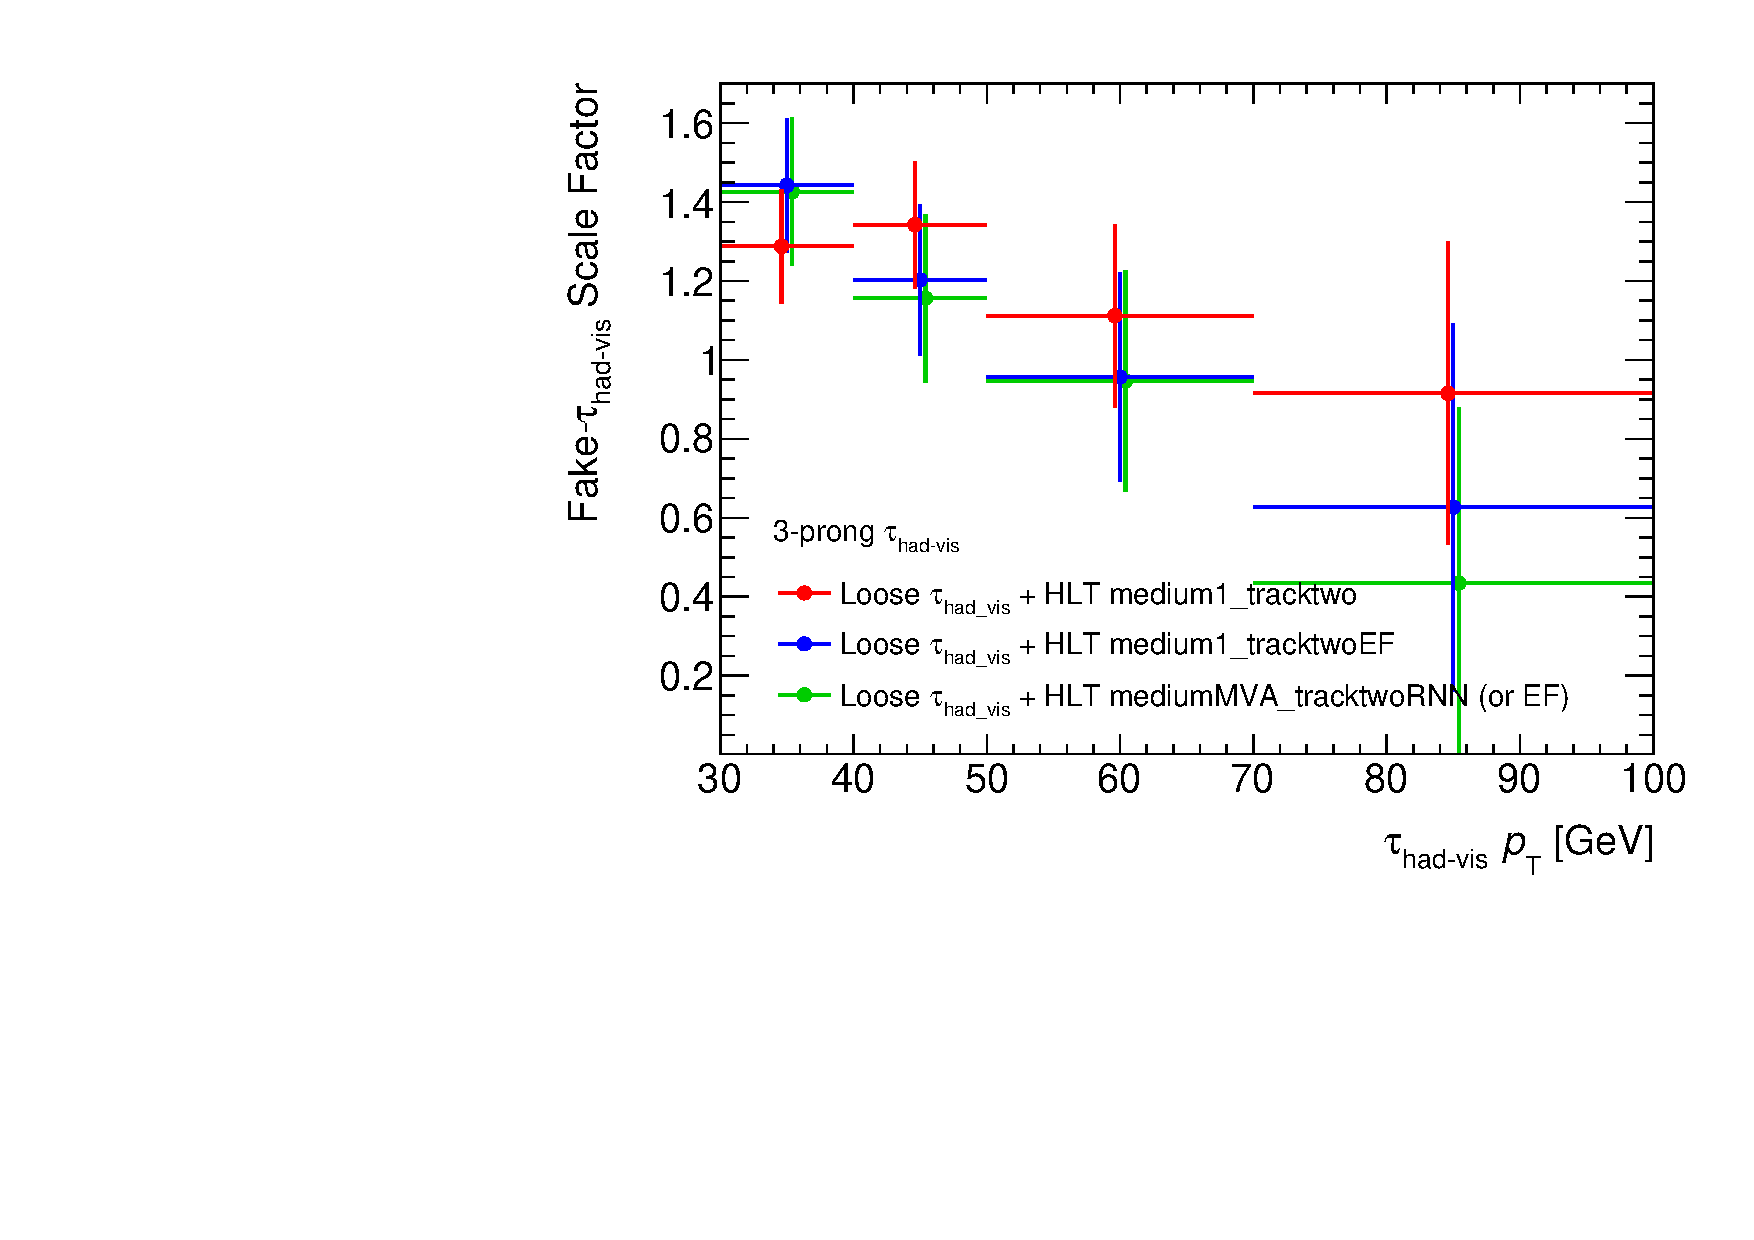
\includegraphics[width=\textwidth]{ttbarSF/ttbarSF_tau25_3p}
    \caption{}
    \label{fig:ttbarSF_postfit_SF_d}
  \end{subfigure}

  \caption[\Faketauhadvis SFs for different \tauid criteria.]{\Faketauhadvis SFs
    for different \tauid criteria. Figures~(a) and (b) compare the SFs with and
    without tau identification at the HLT. The effect of different
    \tauhadvis-triggers on the extracted SFs is shown in Figures~(c) and (d). In
    all cases, the last bin summarises the SFs for \tauhadvis candidates with
    $\pT \geq \SI{70}{\GeV}$. The markers are shifted from their geometrical bin
    centres for illustration purposes only.}%
  \label{fig:ttbarSF_postfit_SF}
\end{figure}

The fit model and the corresponding fit results are checked by comparing the
post-fit predictions of the model with the observed data in all \tauhadvis
candidate \Ntracks and \pT regions. In addition, pulls and constraints of
nuisance parameters, and correlations between nuisance parameters and the POIs
are inspected. Exemplary post-fit predictions of the model are shown in
\Cref{fig:ttbarSF_postfit_ptmtw} in terms of the \pT of \tauhadvis candidates
and \mTW in the SF-CR after requiring events to pass the
\texttt{HLT\_tau25\_medium1\_tracktwo} trigger and trigger-matching.

\begin{figure}[htbp]
  \centering

  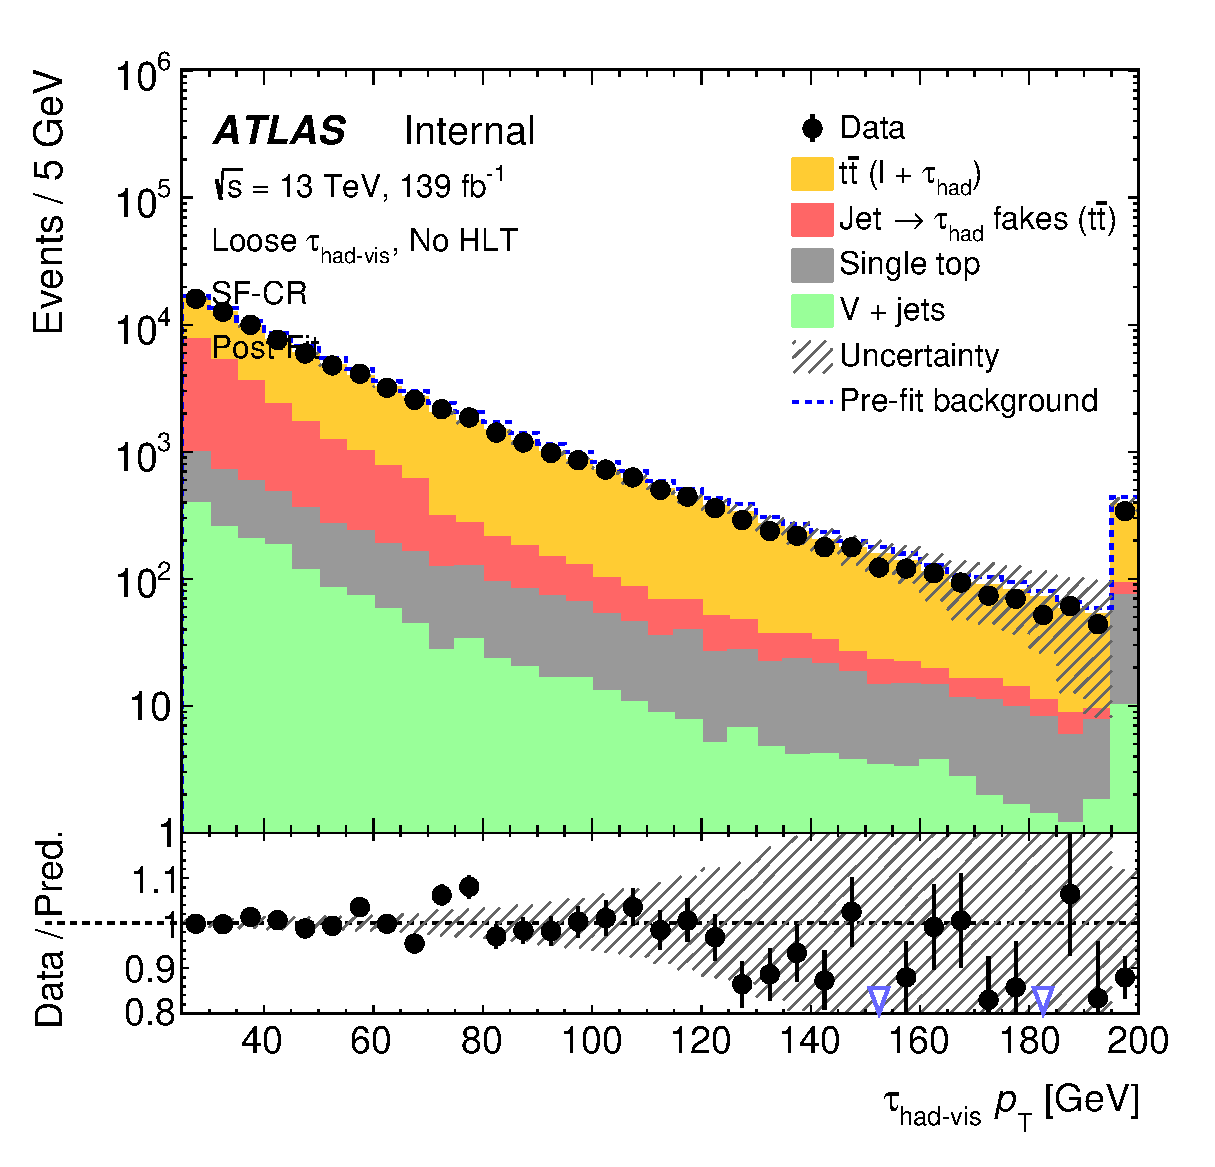
\includegraphics[width=0.49\textwidth]{ttbarSF/postfit_sfcr/PTVR_postFit}
  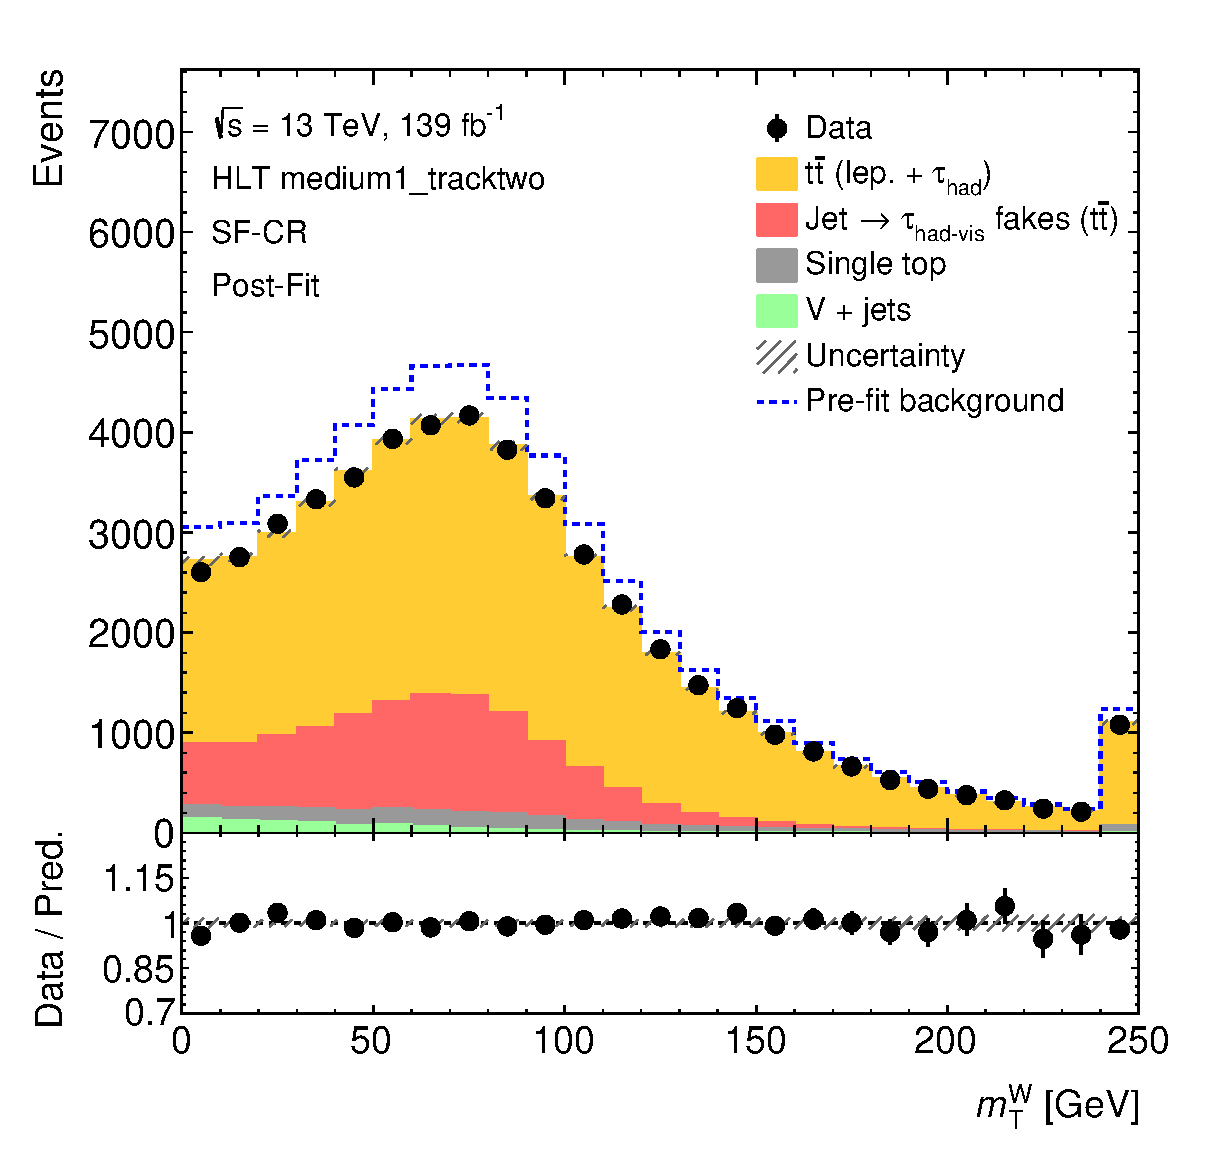
\includegraphics[width=0.49\textwidth]{ttbarSF/postfit_sfcr/MTWVR_postFit}

  \caption[Post-fit distributions of \tauhadvis candidate \pT and \mTW in the
  SF-CR.]{Post-fit distributions of \tauhadvis candidate \pT and \mTW in the
    SF-CR for events passing the \texttt{HLT\_tau25\_medium1\_tracktwo} trigger
    and trigger-matching. Both distributions are inclusive in \Ntracks and \pT
    of \tauhadvis candidates. Events with \tauhadvis \pT (\mTW) larger than
    \SI{200}{\GeV} (\SI{250}{\GeV}) are included in the last bin. The
    uncertainty band contains all statistical and systematic uncertainties,
    including post-fit uncertainties on \faketauhadvis SFs and on the overall
    \ttbar normalisation factor.}%
  \label{fig:ttbarSF_postfit_ptmtw}
\end{figure}

The post- and pre-fit values of all nuisance parameters agree within their
uncertainties. Few instances are observed where the SF measurement puts more
stringent constraints on the values of nuisance parameters than expected from
the prior estimation of the associated uncertainty. These cases are the
\pTmissAbs scale uncertainty, the \ttbar modelling uncertainties resulting from
comparison with alternative ME/PS generators, and the \tauhadvis energy scale
uncertainty. The constraints on these parameters tend to be moderate with ratios
of post- to pre-fit uncertainties above \SI{70}{\percent}. Due to the
sensitivity of the \mTW discriminant to the modelling of \pTmissAbs and the
abundance of \ttbar events in the SF-CR, the fit is expected to have some power
to constrain the associated nuisance parameters. Moreover, the \tauhadvis energy
scale uncertainties are derived from $Z \ra \tau_{\mu} \tauhad$ tag-and-probe
measurements~\cite{ATLAS-CONF-2017-029} that provide probe \tauhadvis with
smaller transverse momenta than the ones produced in \ttbar events. With the SF
measurement being performed in \Ntracks and \pT bins of the \tauhadvis candidate
and targeting \ttbar events, constraints on the \tauhadvis energy scale in the
SF measurement are expected.

% Pulls and constraints of nuisance parameters are examined for all scale factor
% measurements. The nuisance parameter estimates agree within uncertainties with
% the central values of their auxiliary measurements. Few instances are observed
% where the scale factor measurement puts more stringent constraints on nuisance
% parameters than expected from the prior estimation of the associated
% uncertainty. All constrained parameters have post-fit uncertainties larger
% than \SI{70}{\percent} with respect to the uncertainty prior to the fit,
% indicating only mild constraints.

% The largest nuisance parameter constraints, in the following given as the
% ratio of post- to pre-fit uncertainty, are observed for the \pTmissAbs scale
% uncertainty~(\SI{70}{\percent}), the ME / PS modelling uncertainties on
% \ttbar~(\SI{75}{\percent}), and \tauhadvis energy scale
% uncertainty~(\SI{80}{\percent}).  The \mTW discriminant is sensitive to the
% modelling of \pTmissAbs, thus some power to constrain nuisance parameters
% related to the modelling of \pTmissAbs in simulation is expected. Similarly,
% the SF-CR selects a large number of \ttbar events with high purity,
% consequently allowing to constrain the modelling uncertainties that are
% derived from two-sample comparisons. Finally, the measurements providing
% uncertainties on the \tauhadvis energy scale are performed in
% $Z \ra \tau_{\mu} \tauhad$ tag-and-probe~\cite{ATLAS-CONF-2017-029} which
% provides probe \tauhadvis with a softer transverse momentum spectrum compared
% to \tauhadvis produced in \ttbar events. With the binning of the measurement
% in \tauhadvis \pT, it is expected that the uncertainties on the \tauhadvis
% energy scale, particularly at high \tauhadvis~\pT, can be constrained by this
% measurement.

The limited discrimination power of \mTW in distinguishing \ttbar events with
and without \faketauhadvis leads to large anti-correlations between
\faketauhadvis SFs and the \ttbar normalisation factor. Due to this coupling,
positive correlations are induced between the SFs themselves. This is
illustrated in \Cref{fig:ttbarSF_corr_matrix} for an exemplary SF measurement.

% The fit model introduces large anti-correlations between the overall \ttbar
% normalisation and the extracted scale factors for \ttbar with \faketauhadvis. An
% exemplary correlation matrix for one measurement is shown
% in~\Cref{fig:ttbarSF_corr_matrix} showing the most relevant correlations between
% parameters of interest and nuisance parameters.  The anti-correlations are a
% result of the limited discrimination power of \mTW in distinguishing between
% \ttbar with true- and \faketauhadvis, which is especially poor for low
% \tauhadvis transverse momenta. Thus a change in the overall \ttbar
% normalisation, affecting both \ttbar with true and \faketauhadvis, can be
% partially compensated by an increase in the \faketauhadvis scale factors. This
% coupling between \faketauhadvis scale factors and \ttbar normalisation
% introduces large positive correlations also between the scale factors
% themselves.

\begin{figure}[htbp]
  \centering

  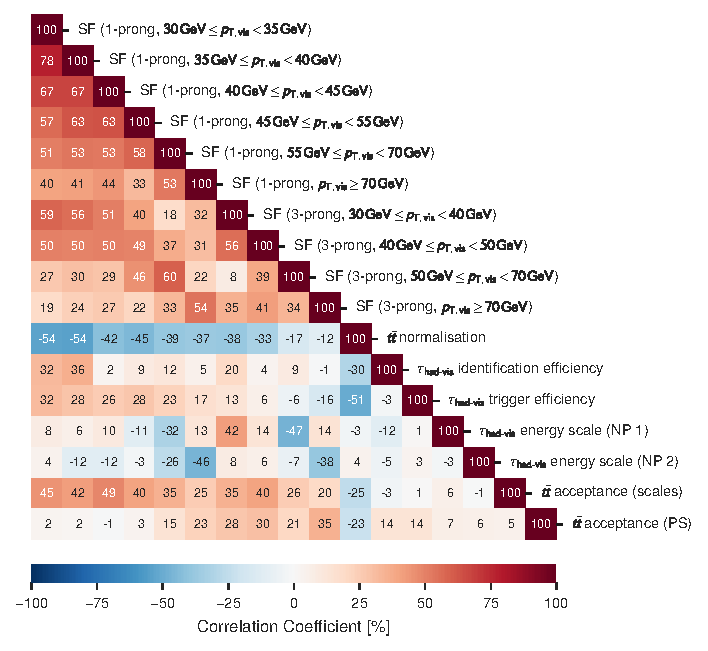
\includegraphics[scale=0.88]{ttbarSF/correlation_matrix}

  \caption[Post-fit correlation matrix between selected parameters of the
  \faketauhadvis SF measurement for the \texttt{HLT\_tau25\_medium1\_tracktwo}
  trigger.]{Post-fit correlation matrix between selected parameters of the
    \faketauhadvis SF measurement for the \texttt{HLT\_tau25\_medium1\_tracktwo}
    trigger. A reduced number of NPs is shown for illustration purposes. NPs are
    included if the absolute value of its correlation coefficient with at least
    one POI exceeds \SI{30}{\percent}.}%
  \label{fig:ttbarSF_corr_matrix}
\end{figure}

Correlations between the measured SFs need to be taken into account when
propagating the uncertainties on the SFs to the estimate of the \ttbarFakes
background in the \hadhad SR. This is achieved by providing a set of
decorrelated variations of the measurement that explains the total uncertainty
of all measured SFs. These variations can be used to propagate the uncertainties
to the background estimate without having to account for correlations.

A decorrelated set of variations is obtained by performing a linear
transformation of the $N$ measured SFs. The transformation is obtained by
diagonalising the post-fit SF covariance matrix, yielding a set of eigenvectors
and eigenvalues. The eigenvectors provide an alternative basis in which the
measurement is described by $N$~linear combinations of SFs with diagonal
covariance matrix. The eigenvalues correspond to the variance explained by
certain linear combinations of SFs.
% The covariance between two different linear combinations is
% zero by construction and the eigenvalues describe the variance of
% individual linear combinations.
In the frame with diagonal covariance matrix, the SF measurement is varied by
performing $\pm 1 \sigma$ variations, then transforming the resulting variations
back to the original, physically interpretable frame. This procedure yields $N$
systematic variations of the SF measurement, each with an up- and
down-variation. The variations are ordered by descending variance in the
diagonal frame, yielding variations that are roughly decreasing in their impact
on the total \ttbarFakes background estimate. An example of the results of the
decorrelation procedure is shown in~\Cref{fig:ttbarSF_eigenvariations}. The
effect of large correlations between SFs can be observed in the leading
variation (\texttt{EIGEN0}) as a systematic shift of the variation in all bins
with respect to the nominal result. In contrast, the variation explaining the
least variance (\texttt{EIGEN9}) only alters the SFs for 1-prong \faketauhadvis
with low transverse momenta.

\begin{figure}[htbp]
  \centering

  \begin{subfigure}[t]{.495\textwidth}
    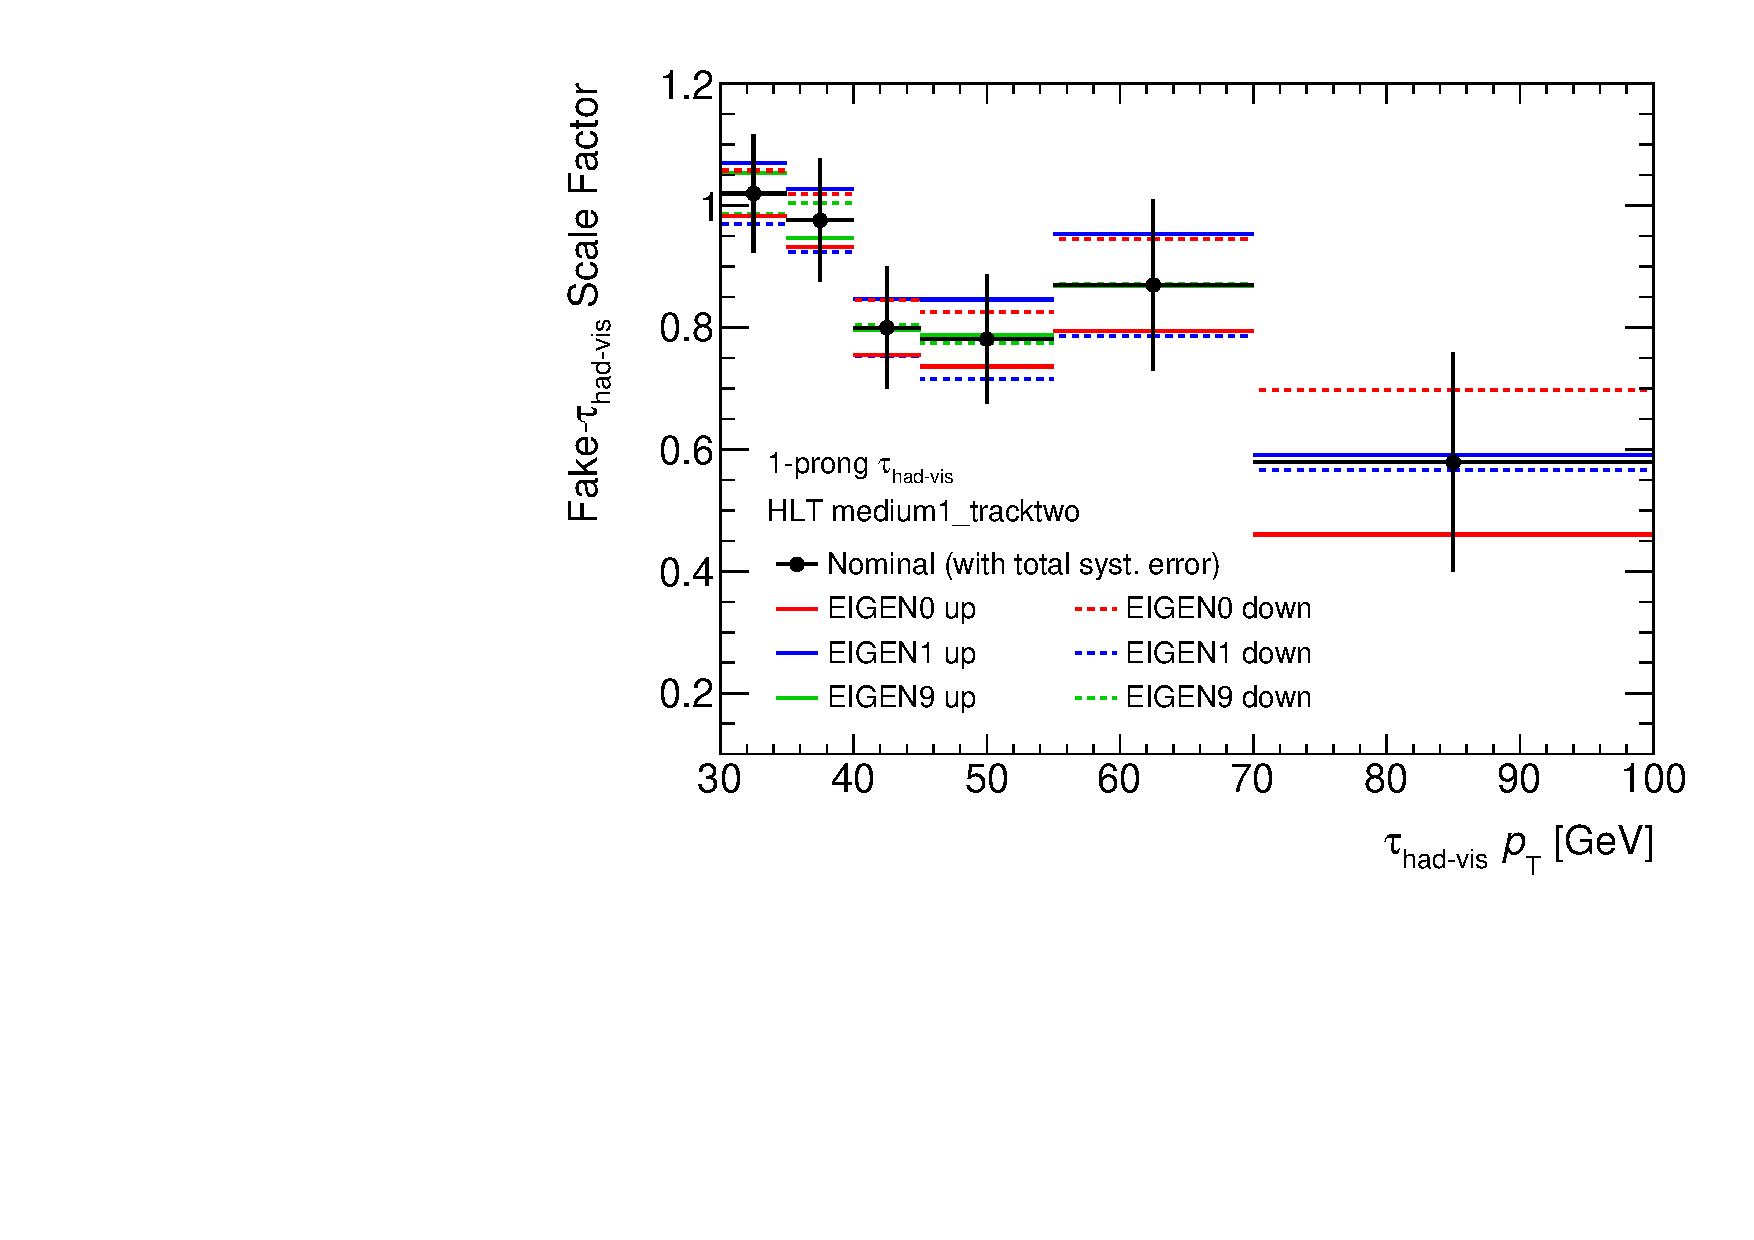
\includegraphics[width=\textwidth]{ttbarSF/ttbarSF_eigvar_1p}
    \caption{1-prong \tauhadvis}%
    \label{fig:ttbarSF_eigenvariations_1p}
  \end{subfigure}\hfill%
  \begin{subfigure}[t]{.495\textwidth}
    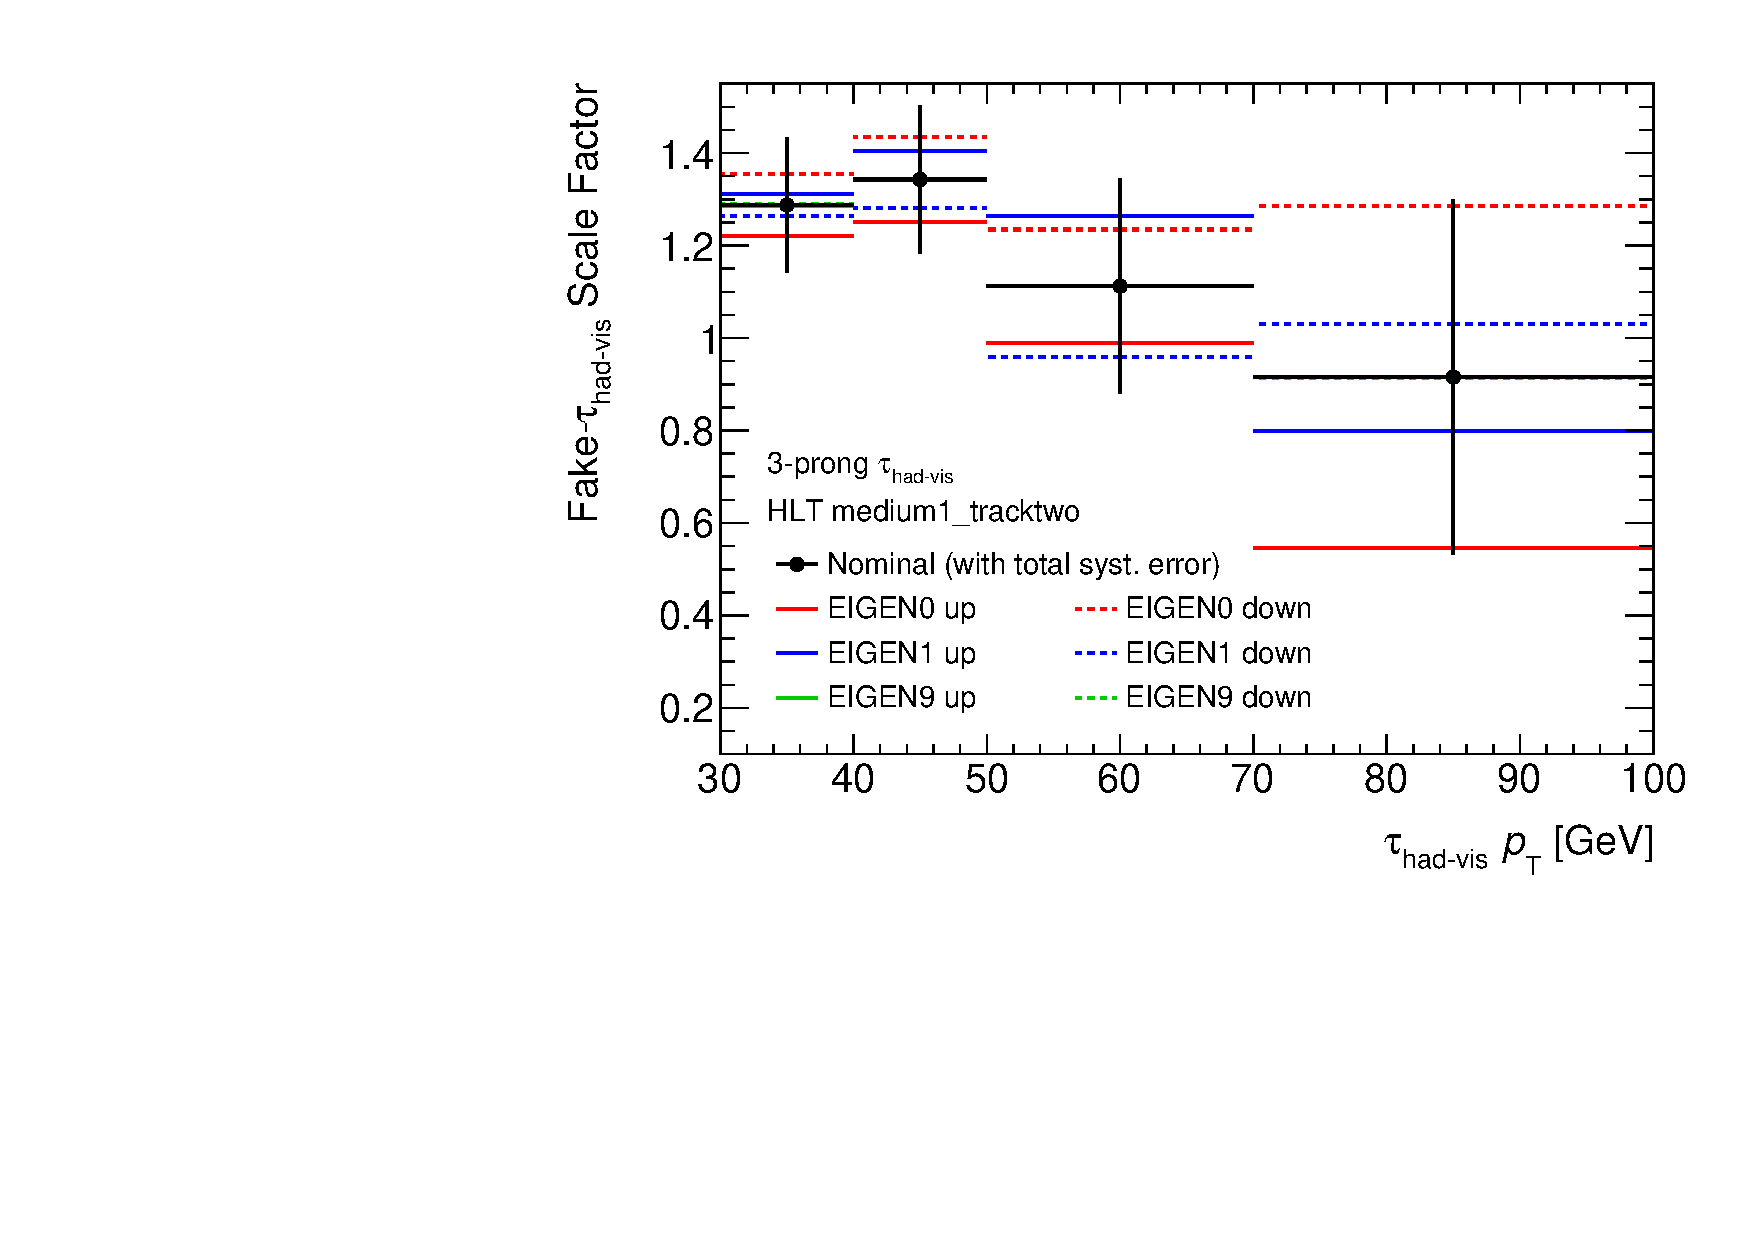
\includegraphics[width=\textwidth]{ttbarSF/ttbarSF_eigvar_3p}
    \caption{3-prong \tauhadvis}%
    \label{fig:ttbarSF_eigenvariations_3p}
  \end{subfigure}

  % Adding the deviations of all variations (\texttt{EIGEN0}--\texttt{EIGEN9})
  % from the nominal result in quadrature recovers the total uncertainty.

  \caption[Systematic variations of the \faketauhadvis SFs for the
  \texttt{HLT\_tau25\_medium1\_tracktwo} trigger.]{\Faketauhadvis SF variations
    resulting from the decorrelation procedure applied to the measurement for
    the \texttt{HLT\_tau25\_medium1\_tracktwo} trigger. The two variations
    leading in the explained variance (\texttt{EIGEN0} and \texttt{EIGEN1}) as
    well as the variation explaining the least variance (\texttt{EIGEN9}) are
    shown.}%
  \label{fig:ttbarSF_eigenvariations}
\end{figure}


\subsubsection{Application of \Faketauhadvis Scale Factors in the \hadhad
  Channel}

The \ttbarFakes background in the SR of the \hadhad channel is estimated by
applying \faketauhadvis SFs to \ttbar events from simulation with at least one
\faketauhadvis. These events are required to pass the SR selection criteria of
the \hadhad channel, including the trigger selection described
in~\Cref{sec:trigger}. The SFs are chosen depending on the trigger category and
whether the \faketauhadvis is the \tauhadvis candidate leading in \pT,
sub-leading in \pT, or both selected candidates are \faketauhadvis. When both
\tauhadvis candidates are originating from quark- or gluon-initiated jets, the
SF correction is assumed to factorise and the product of SFs is assigned as an
event-level weight.

In events selected by DTTs, both \tauhadvis candidates have to fulfil the
trigger-level identification requirements. In this case the set of SFs is chosen
according to the trigger chain that selected the event, independently of which
\tauhadvis candidate is the \faketauhadvis. In contrast, only one \tauhadvis
candidate has to fulfil the trigger-level requirements in events selected by
STTs. For STT events, it is assumed that the \tauhadvis candidate leading in \pT
is the one satisfying the trigger conditions. This assumption is correct for
more than \SI{99}{\percent} \ttbar events containing \faketauhadvis in the STT
category. Therefore, SFs measured for \faketauhadvis after trigger-matching are
applied when the leading \tauhadvis candidate is the \faketauhadvis; SFs derived
without trigger-matching are applied when the sub-leading \tauhadvis candidate
is the \faketauhadvis. Similar to the DTT case, if the \tauhadvis candidate
leading in \pT is the \faketauhadvis, then the set of SFs that corresponds to
the trigger chain that selected the event is used. The event weight calculation
is summarised in~\Cref{tab:ttbarSF_application_rule}.

\begin{table}[htbp]
  \centering

  \caption[Event weights for the application of SFs to \ttbarFakes events in
  simulation.]{Event weights for the application of SFs to \ttbarFakes events in
    simulation. Events are categorised by whether the leading \tauhadvis
    candidate~($\tau_{\text{lead.}}$), sub-leading \tauhadvis
    candidate~($\tau_{\text{subl.}}$), or both \tauhadvis candidates are
    \faketauhadvis. SFs for \faketauhadvis without identification at
    trigger-level are denoted by $\text{SF}_{\text{loose}}$. SFs for
    \faketauhadvis with both offline and trigger-level identification
    requirements are denoted by $\text{SF}_\text{loose+trig.}$.}%
  \label{tab:ttbarSF_application_rule}

  \resizebox{\textwidth}{!}{
    \begin{tabular}{cc@{\hskip 2em}rcl@{\hskip 2em}rcl}
  \toprule
  $\tau_{\text{lead.}}$ & $\tau_{\text{subl.}}$ & \multicolumn{3}{c}{Event weight (STT)} & \multicolumn{3}{c}{Event weight (DTT)} \\
  \midrule
  true & fake & $1$ & $\times$ & $\text{SF}_\text{loose}(\tau_{\text{subl.}})$
              & $1$ & $\times$ & $\text{SF}_\text{loose+trig.}(\tau_{\text{subl.}})$ \\[0.2em]

  fake & true & $\text{SF}_\text{loose+trig.}(\tau_{\text{lead.}})$ & $\times$ & $1$
              & $\text{SF}_\text{loose+trig.}(\tau_{\text{lead.}})$ & $\times$ & $1$ \\[0.2em]

  fake & fake & $\text{SF}_\text{loose+trig.}(\tau_{\text{lead.}})$ & $\times$ & $\text{SF}_\text{loose}(\tau_{\text{subl.}})$
              & $\text{SF}_\text{loose+trig.}(\tau_{\text{lead.}})$ & $\times$ & $\text{SF}_\text{loose+trig.}(\tau_{\text{subl.}})$ \\
  \bottomrule
\end{tabular}

%%% Local Variables:
%%% mode: latex
%%% TeX-master: "../phd_thesis"
%%% End:

  }
\end{table}


\subsubsection{Uncertainties on the \ttbarFakes Background in the \hadhad
  Channel}

In addition to the uncertainties originating from the SF measurement, two other
sources of uncertainties are considered. First, an uncertainty accounting for a
possible bias in the estimated SFs due to trigger efficiency turn-on effects
arising from \tauhadvis \pT (\ET) thresholds at the HLT (L1 trigger) is
determined. Second, an uncertainty on the extrapolation of the measured SFs from
$\ell + \tauhadvis$ final states to final states with two \tauhadvis is derived.

A systematic uncertainty accounting for the effect of \tauhadvis \pT (\ET)
thresholds at the HLT~(L1 trigger) on the \faketauhadvis SFs is estimated. The
nominal SF measurement is performed using \tauhadvis-triggers with thresholds of
$\pT > \SI{25}{\GeV}$ at the HLT and $\ET > \SI{12}{\GeV}$ at the L1
trigger~(\texttt{tau25}). However, triggers with larger thresholds are also
employed in the \hadhad channel. For example, thresholds of
$\pT > \SI{35}{\GeV}$ at the HLT and $\ET > \SI{20}{\GeV}$ at the L1 trigger
(\texttt{tau35}) are applied to the leading \tauhadvis candidate selected by
DTTs. The application of SFs measured for \texttt{tau25} triggers to
\faketauhadvis that are required to pass a \texttt{tau35} trigger can introduce
a bias due to differences in selection efficiency between both triggers. This
effect is only relevant for \faketauhadvis with transverse momenta close to the
\pT~threshold of the \texttt{tau35} trigger, i.e.\
\SIrange[range-phrase=--]{40}{50}{\GeV} for 1-prong candidates and
\SIrange[range-phrase=--]{40}{60}{\GeV} for 3-prong candidates. For
\faketauhadvis with larger transverse momenta, the differences between triggers
become negligible.

% The difference in trigger efficiency between \texttt{tau25} and \texttt{tau35}
% is studied in simulated \ttbarFakes events in the SF-CR. Only events with
% \tauhadvis candidates with $\pT > \SI{40}{\GeV}$ are considered. After this
% selection, \SI{95}{\percent} (\SI{85}{\percent}) of \faketauhadvis
% reconstructed as 1-prong (3-prong) candidates selected by \texttt{tau25} also
% pass the \texttt{tau35} triggers. The difference in \faketauhadvis selected by
% the \texttt{tau25} and \texttt{tau35} triggers is a potential source of bias
% in the estimation of the \ttbarFakes background. For \faketauhadvis
% reconstructed as 1-prong (3-prong) candidates and with $\pT > \SI{50}{\GeV}$
% ($\pT > \SI{60}{\GeV}$), the differences in \faketauhadvis selected by
% \texttt{tau25} and \texttt{tau35} become negligible.

An uncertainty is assigned to SFs applied to \faketauhadvis that are required to
pass a \texttt{tau35} trigger if the transverse momentum of the \faketauhadvis
is close to the \pT~threshold of the trigger. In particular, the uncertainty is
only applied for 1-prong (3-prong) \faketauhadvis with transverse momenta below
\SI{50}{\GeV} (\SI{60}{\GeV}). The size of the uncertainty is estimated by
repeating the SF measurement for the \texttt{tau35} triggers and comparing with
the nominal set of SFs. This comparison is performed for all trigger chains
employed in the analysis, resulting in a relative uncertainty of approximately
\SI{6}{\percent} for all triggers considered in this search.

% \begin{table}[htbp]
%   \centering

%   \caption{Size of the uncertainty comparing scale factors measured
%     for triggers with $\pTHLT > \SI{25}{\GeV}$ and
%     $\pTHLT > \SI{35}{\GeV}$ thresholds. The uncertainty is given
%     relative to all events from \ttbar in the \hadhad channel signal
%     region where the leading \tauhadvis is a \faketauhadvis with \pT
%     close to the \SI{40}{\GeV} threshold.}%
%   \label{tab:ttbarSF_tau25_35_uncertainty}

%   \begin{tabular}{lcc}
  \toprule
  & {1-prong \tauhadvis} & {3-prong \tauhadvis} \\
  & {(40 - 50 GeV)} & {(40 - 60 GeV)} \\
  \midrule
  \texttt{medium1\_tracktwo} (ttbarFT) & $\pm 5.8 \%$ & $\pm 5.5 \%$ \\
  \texttt{medium1\_tracktwo} (ttbarFF) & $\pm 5.9 \%$ & $\pm 5.2 \%$ \\[0.5em]

  \texttt{medium1\_tracktwoEF} (ttbarFT) & $\pm 6.4 \%$ & $\pm 8.1 \%$ \\
  \texttt{medium1\_tracktwoEF} (ttbarFF) & $\pm 6.4 \%$ & $\pm 8.0 \%$ \\[0.5em]

  \texttt{mediumRNN\_tracktwoMVA} (or EF) (ttbarFT) & $\pm 3.8 \%$ & $\pm 2.7 \%$ \\
  \texttt{mediumRNN\_tracktwoMVA} (or EF) (ttbarFF)& $\pm 4.0 \%$ & $\pm 2.6 \%$ \\
  \bottomrule
\end{tabular}

%%% Local Variables:
%%% mode: latex
%%% TeX-master: "../phd_thesis"
%%% End:

% \end{table}

The measurement of the SFs is performed in the SF-CR and applied to events in
the SR of the \hadhad channel. An uncertainty is assigned to account for the
extrapolation of the SF measurement from the SF-CR to the \hadhad SR. The
uncertainties are derived by performing variations of the \ttbar modelling in
simulation and comparing the acceptance of \ttbarFakes events in the SF-CR and
the \hadhad SR. Variations of the matrix element generator, the parton shower
simulation, the renormalisation and factorisation scales, and the modelling of
initial and final state radiation are considered
(cf.~\Cref{app:top_uncertainties}).

The comparison of \ttbarFakes acceptances are performed separately for events in
the \hadhad SR in which the leading \tauhadvis candidate is the \faketauhadvis
(FT~events), the sub-leading \tauhadvis candidate is the \faketauhadvis
(TF~events), and cases in which both candidates are \faketauhadvis
(FF~events). This comparison yields extrapolation uncertainties of
\SI{14}{\percent} for TF~events, \SI{7}{\percent} for FT~events, and
\SI{39}{\percent} for the FF~events. In all cases, the uncertainty is dominated
by the comparison of \PYTHIA[8] and \HERWIG[7] for the simulation of the parton
shower. The large uncertainty on FF~events is expected since the measurement in
the SF-CR can only target events with exactly one \faketauhadvis.

% \begin{align*}
%   N(\ttbarFakes) = \num{2490}
%   \valuesep\numerrt{22}{stat.}%
%   \valuesep\numerrt{210}{meas.}%
%   \valuesep\numerrt{240}{extrapol.}%
%   \valuesep\numerrt{3.6}{trigger threshold} \,\text{.}
% \end{align*}
In the following, the impact of the uncertainties on the total \ttbarFakes
background prediction in the SR of the \hadhad channel is summarised. The
relative uncertainties on the prediction split by uncertainty source are:
\begin{itemize}

\item Uncertainties from the SF measurement:~$\pm \SI{8.5}{\percent}$.

\item Extrapolation uncertainties (SF-CR $\ra$ \hadhad
  SR):~$\pm \SI{9.7}{\percent}$.

\item Uncertainty on SFs due to different \pT (\ET) thresholds of
  \tauhadvis-triggers:~$\pm \SI{0.2}{\percent}$.

\item Statistical uncertainty from finite number of simulated
  events:~$\pm \SI{0.9}{\percent}$.

\end{itemize}
The dominant sources of uncertainty on the prediction of the \ttbarFakes
background are the uncertainties on the SFs from the SF measurement and the
extrapolation uncertainties. Due to the small expected number of FF events in
the \hadhad SR (cf.~\Cref{tab:ttbarSF_yields}), the large extrapolation
uncertainty for FF events has limited impact on the uncertainty of the total
\ttbarFakes prediction.
% The uncertainty accounting for the effects of different \pT~(\ET)~thresholds
% of \tauhadvis-triggers has only a minor impact on the overall \ttbarFakes
% background prediction since only a small fraction of events is affected by
% this uncertainty.
\Cref{tab:ttbarSF_yields} summarises the \ttbarFakes prediction in the \hadhad
SR and compares it to the prediction from simulation without application of
\faketauhadvis SFs.
% Generally, both predictions agree within uncertainties except for the
% FT~component. The predicted number of FT~events is smaller after application
% of \ttbarFake SFs due to SFs being smaller than unity for \faketauhadvis with
% high~\pT.

% The total \ttbarFakes event yield in the \hadhad SR is determined with a
% relative uncertainty of \SI{13}{\percent}, agreeing with the uncorrected
% estimate of the total yield within uncertainties. The expected number of
% \ttbarFakes events is slightly smaller after correction since the measured
% scale factors for high \pT \faketauhadvis tend to be smaller than unity. This
% is also reflected in the larger relative change of the the FT-component (the
% leading \tauhadvis candidate is a \faketauhadvis), for which the
% \faketauhadvis has an average \pT of \SI{65}{\GeV}.

% The SF method described in this section provides a measurement-driven approach
% of estimating the \ttbarFakes background and its uncertainty in the SR of the
% \hadhad channel.  In~\Cref{tab:ttbarSF_yields}, the event yield of \ttbarFakes
% in the \hadhad SR is shown and compared to \ttbar simulation without
% corrections.

\begin{table}[htbp]
  \centering

  % The \ttbarFakes background is split into cases where the sub-leading
  % \tauhadvis candidate is the \faketauhadvis (TF), the leading \tauhadvis
  % candidate is the \faketauhadvis, or both candidate are \faketauhadvis (FF).

  \caption[Expected number of \ttbarFakes events in the \hadhad SR with and
  without application of the \faketauhadvis~SFs.]{Expected number of \ttbarFakes
    events in the \hadhad SR with (right) and without (left) application of the
    \faketauhadvis~SFs. Only MC statistical uncertainties are shown for the
    estimate without application of the \faketauhadvis~SFs. The background
    estimate using the \faketauhadvis~SFs includes statistical uncertainties and
    all systematic uncertainties related to the SF method. Other experimental
    uncertainties are omitted.}%
  \label{tab:ttbarSF_yields}

  % Source:
% https://docs.google.com/spreadsheets/d/1uwVElPaR1HuqEHaL8eAh5pEoGdK2ZBQ8D_Ob8lSSPwE/edit#gid=0

% fSumw[1]=2705.09, x=0.5, error=22.9788

% Only measurement uncertainties
% ttbarSFTF: 1433.95 +- 87.88
% ttbarSFFT: 698.52 +- 72.21
% ttbarSFFF: 358.92 +- 53.50
% Total: 2491.39 +- 21.59 +- 202.99 = 204.13493

\begin{tabular}{
  l
  @{\hskip 16pt}
  S[table-format=4.0(2)]
  @{\hskip 16pt}
  S[table-format=4.0(3)]
  }
  \toprule
  & \multicolumn{2}{c}{Expected number of events (pre-fit)} \\
  \cmidrule{2-3}
          & {Simulation} & {Simulation with} \\
  Process &              & {\faketauhadvisC SF}  \\
  \midrule
  \ttbar + \faketauhadvisC (TF) & 1428 +- 16 & 1430 +- 230 \\
  \ttbar + \faketauhadvisC (FT) & 854 +- 13 & 699 +- 88 \\
  \ttbar + \faketauhadvisC (FF) & 423 +- 12 & 360 +- 160 \\
  \midrule
  \ttbar + \faketauhadvisC (total) & 2705 +- 23 & 2490 +- 320 \\
  \bottomrule
\end{tabular}

%%% Local Variables:
%%% mode: latex
%%% TeX-master: "../phd_thesis"
%%% End:

\end{table}

% The uncertainties originating from the SF measurement in the SF-CR (meas.) and
% the extrapolation uncertainties (extrapol.) have uncertainties of similar
% size. The extrapolation uncertainty is dominated by the comparison of
% different parton shower programs. The \faketauhadvis \pT-dependent PS
% uncertainty, affecting the TF- and FT-components of the background, has a
% particularly large impact on the TF contribution. This is due to the large
% uncertainty for 1-prong \faketauhadvis candidates, making up $\frac{3}{4}$ of
% \faketauhadvis in \ttbar, at low transverse momenta as shown
% in~\Cref{fig:ttbarSF_extrapol_shape_a}. Due to the momentum ordering, the
% average \faketauhadvis \pT in \ttbarFakes (TF) is approximately \SI{40}{\GeV}.

% Statistical uncertainties from the finite number of simulated events (stat.)
% and the uncertainty based on the comparison of different trigger thresholds
% (trigger threshold) have negligible impact on the total yield in the \hadhad
% SR.

% Measurement uncertainties on total yield are highly correlated: ca.
% 90% PS uncertainty for 1-prong taus is anti-correlated due to sign-change of uncertainty


\subsubsection{Estimation of \Faketauhadvis Scale Factors for Anti-\tauhadvis}

The estimation of the \multijet background in the \hadhad SR, which is described
in~\Cref{sec:bkg_hadhad_ff}, requires a large subtraction of \ttbarFakes events
in a region defined by the presence of an \antitau
(cf.~\Cref{sec:object_reconstruction}). The SF method is extended to \antitau to
provide uncertainties on this subtraction.
% in the 2 $b$-tag \antiid CR for \tauhadvis candidates with OS electric
% charge. The SF method for estimating the \ttbarFakes background is extended to
% the \antiid region to provide uncertainties on the subtraction performed as
% part of the \multijet estimation.

The SF measurement is repeated using the same SF-CR definition except for
requiring an \antitau instead of a \tauhadvis candidate passing loose
identification.
% inverting the \tauhadvis identification requirement applied during offline
% event reconstruction. Instead of \tauhadvis passing the loose \tauid working
% point, \tauhadvis are required to fail the loose working point but exceed an
% RNN \tauid score threshold of \num{0.01}. The same requirements from the
% ID-region measurement regarding the reconstruction and identification of
% \tauhadvis at the HLT are imposed.\todo{Already explained (object selection)}
This inversion of the \tauid requirement rejects most \ttbar events with
true-\tauhadvis, yielding a region with \ttbarFakes purity of about
\SI{80}{\percent}. Trigger-matching of the \antitau to a \tauhadvis at the HLT
reduces the \ttbarFakes yield by about \SI{80}{\percent} due to the
trigger-level identification requirements; however, only a mild decrease in
\ttbarFakes purity by about 5 percentage points is observed.
% remains largely unchanged.

A reduced set of experimental uncertainties is used for this measurement due to
practical limitations in the dataset preparation for the
$\ell + \text{anti-}\tauhadvis$ region. Uncertainties varying the four-momentum
of reconstructed objects are omitted except uncertainties on the \tauhadvis
energy scale. Other uncertainties that can be expressed by alternative event
weights, for example uncertainties on tagging efficiencies, are considered. Due
to this constraint, the total deviation of the central value of the SFs from
unity is assigned as an additional uncertainty on the measured SFs for \antitau.

The measured SFs for \antitau are shown in~\Cref{fig:ttbarSF_antiid_SF}. The SFs
are generally within \SI{20}{\percent} of unity. The same decorrelation
technique is used to propagate the measurement uncertainties when applying the
SFs to \antitau in the \hadhad channel. The context and impact of the SFs for
\antitau on the \multijet estimate is discussed in \Cref{sec:bkg_hadhad_ff}.

\begin{figure}[htbp]
  \centering

  \begin{subfigure}[t]{.495\textwidth}
    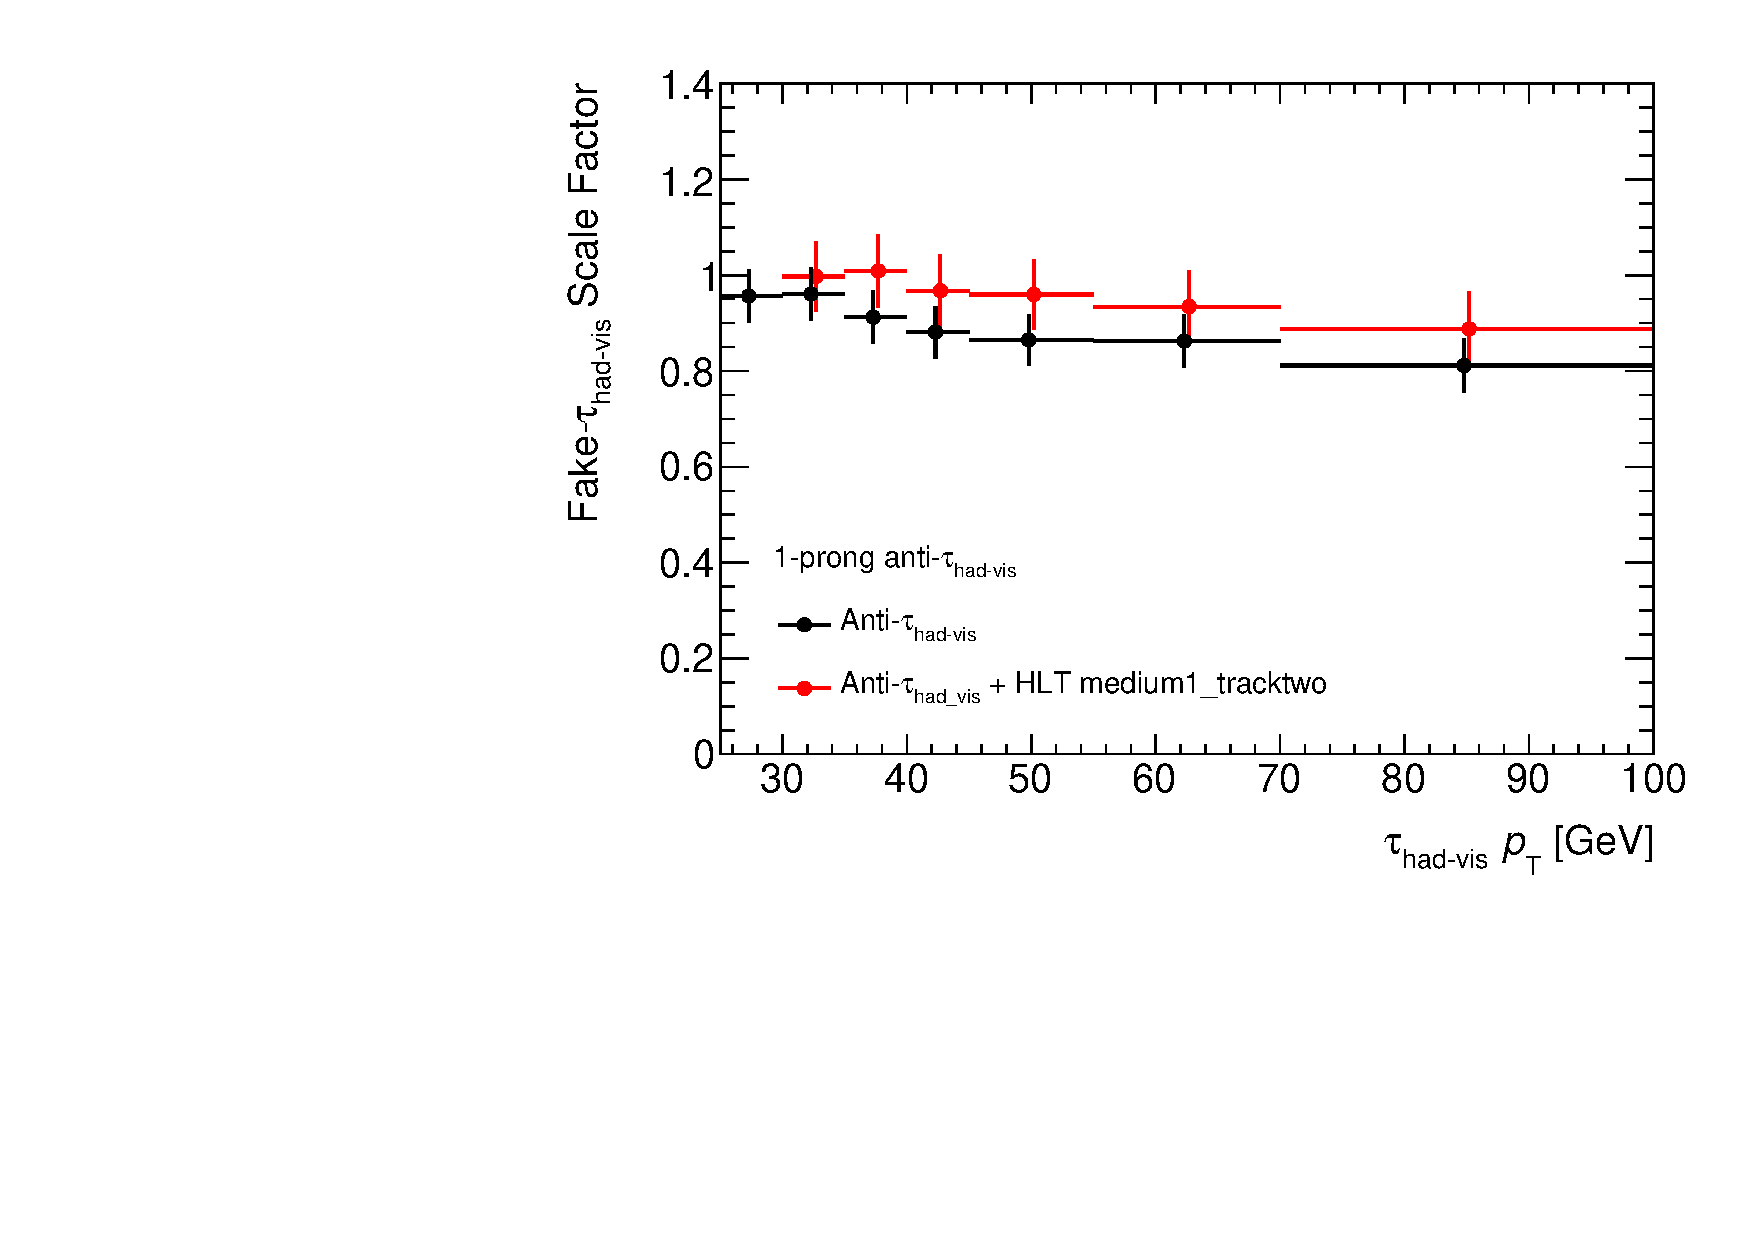
\includegraphics[width=\textwidth]{ttbarSF/scale_factors/ttbarSF_antitau_offl_tau25_1p}
    \caption{}
    \label{fig:ttbarSF_antiid_SF_a}
  \end{subfigure}\hfill%
  \begin{subfigure}[t]{.495\textwidth}
    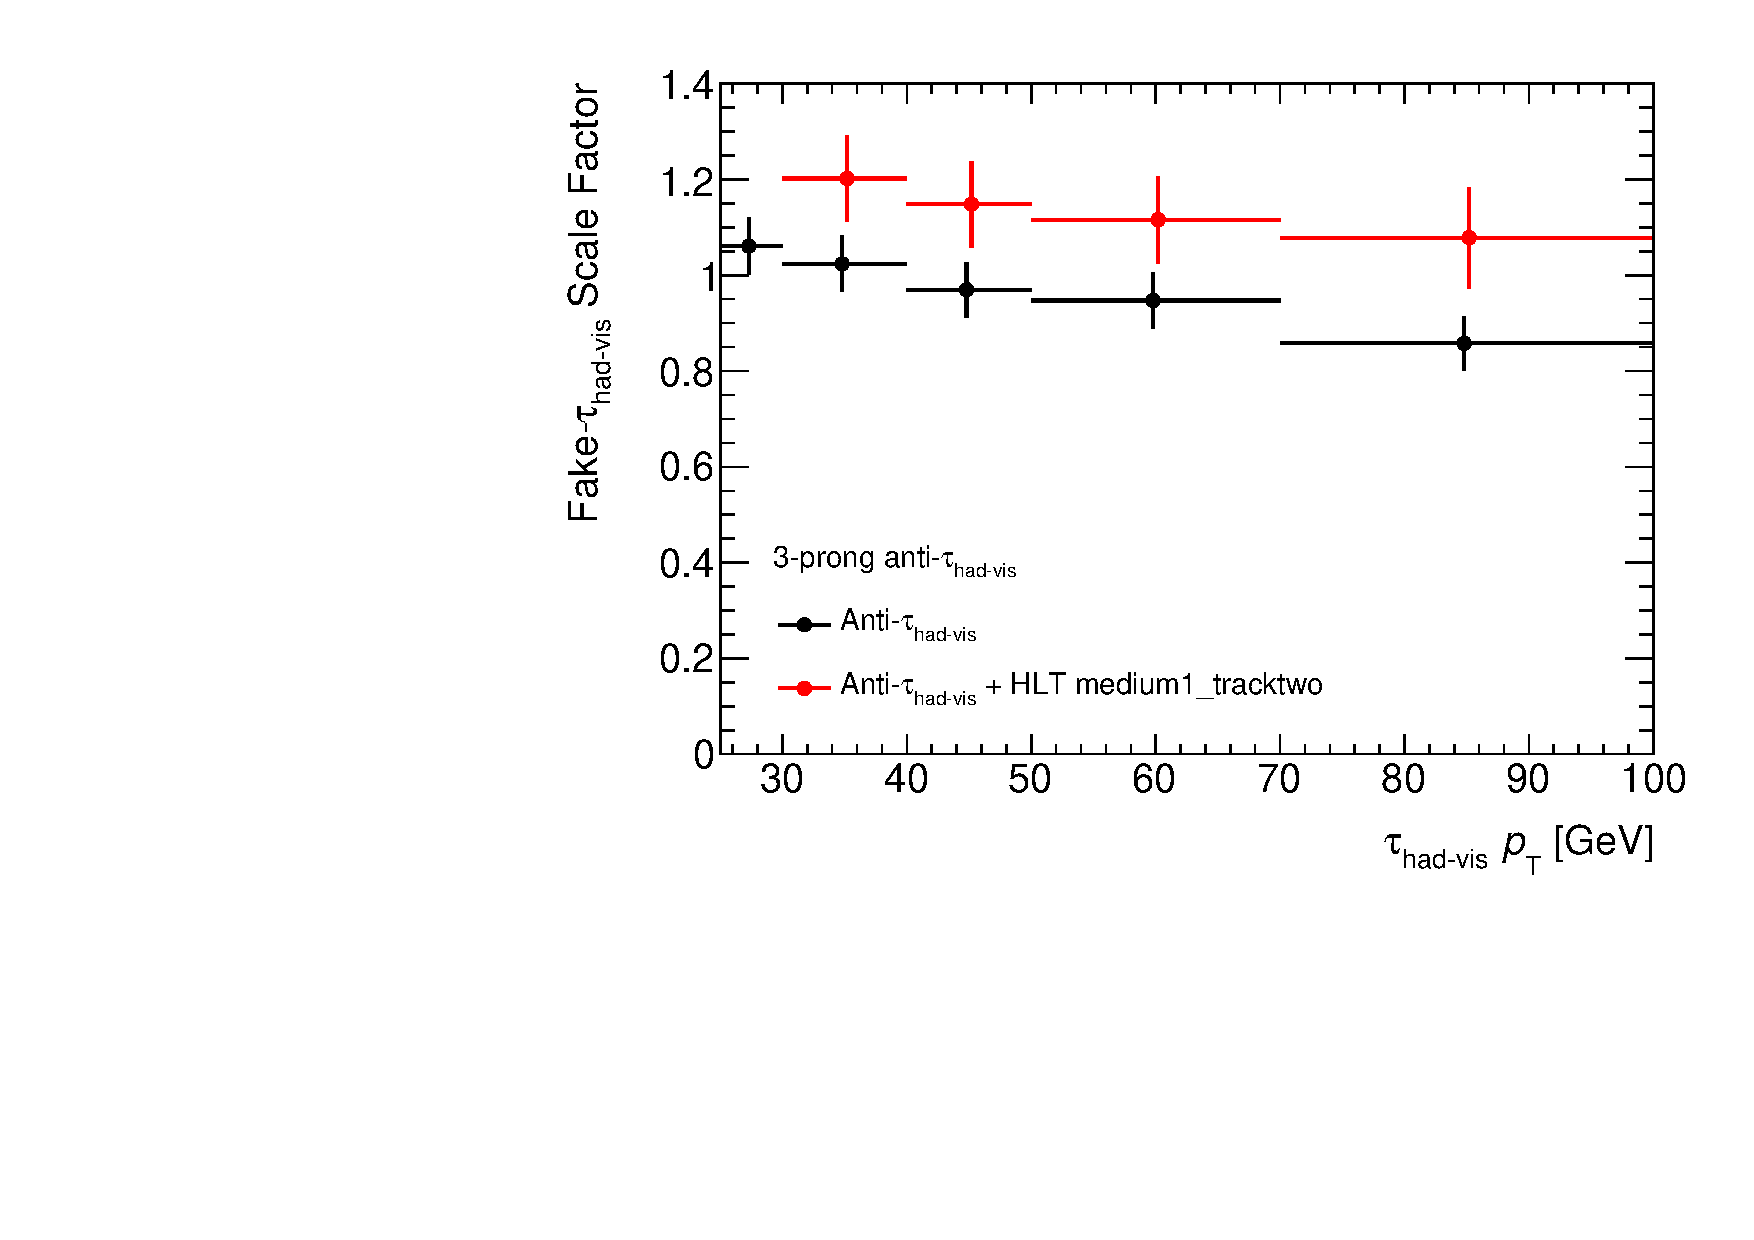
\includegraphics[width=\textwidth]{ttbarSF/scale_factors/ttbarSF_antitau_offl_tau25_3p}
    \caption{}
    \label{fig:ttbarSF_antiid_SF_b}
  \end{subfigure}

  \begin{subfigure}[t]{.495\textwidth}
    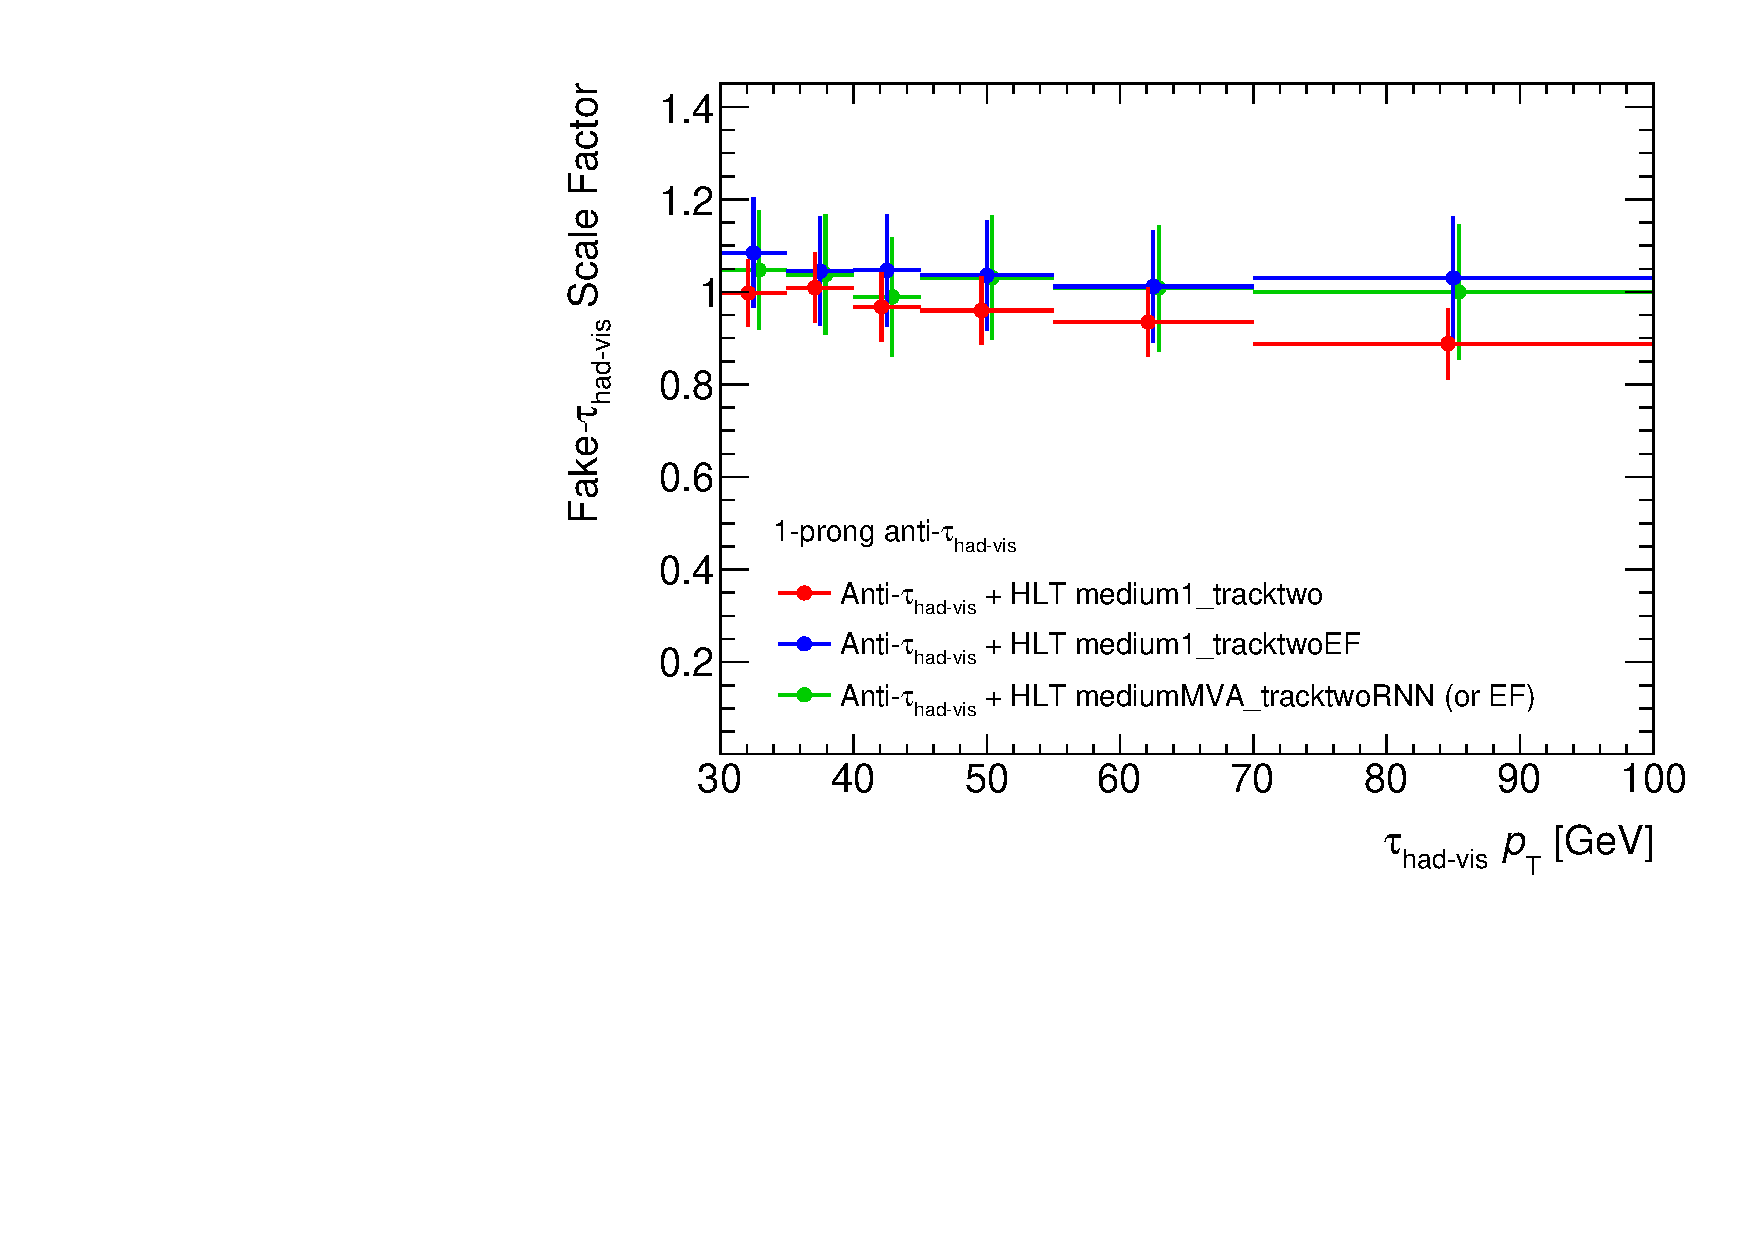
\includegraphics[width=\textwidth]{ttbarSF/scale_factors/ttbarSF_antitau_tau25_1p}
    \caption{}
    \label{fig:ttbarSF_antiid_SF_c}
  \end{subfigure}\hfill%
  \begin{subfigure}[t]{.495\textwidth}
    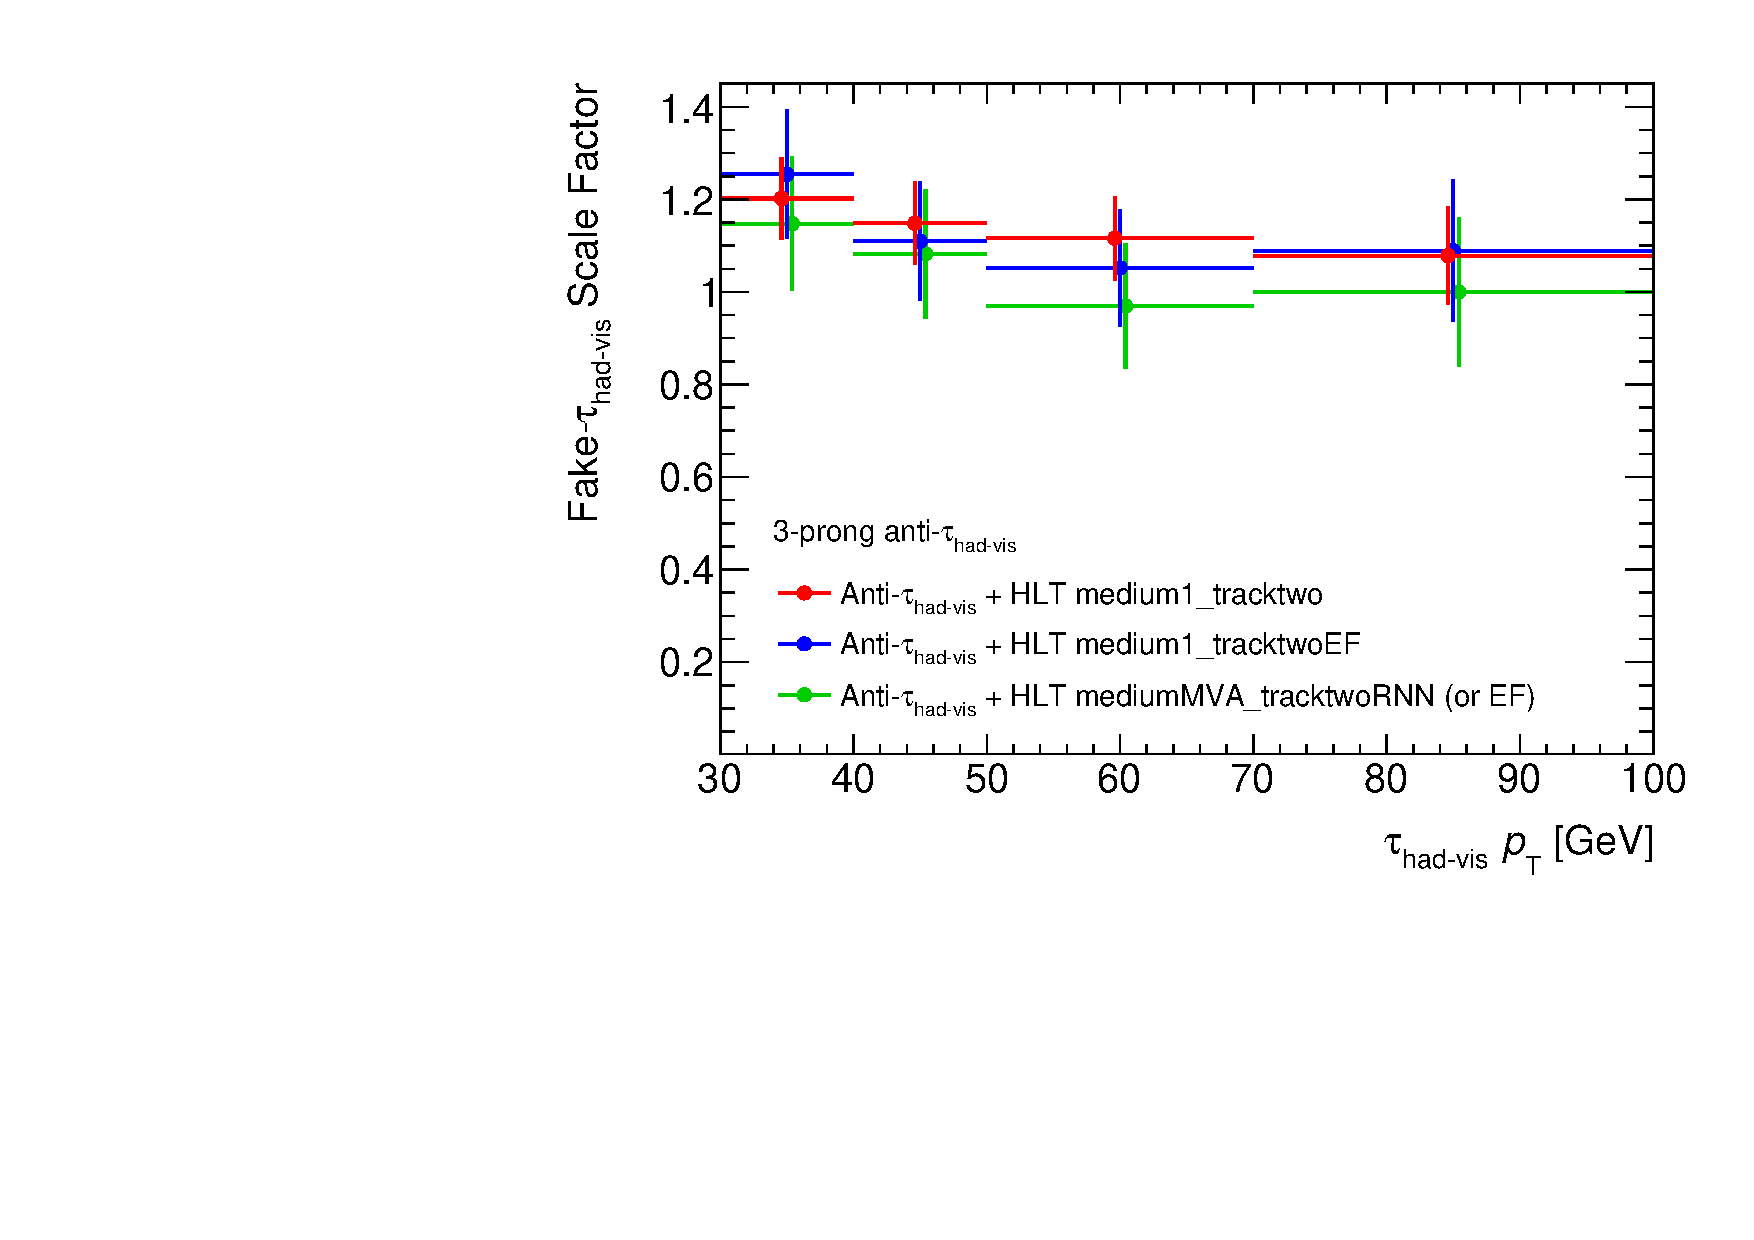
\includegraphics[width=\textwidth]{ttbarSF/scale_factors/ttbarSF_antitau_tau25_3p}
    \caption{}
    \label{fig:ttbarSF_antiid_SF_d}
  \end{subfigure}

  \caption[\Faketauhadvis SFs for anti-\tauhadvis and different \tauid criteria
  applied at trigger-level.]{\Faketauhadvis SFs for anti-\tauhadvis and
    different \tauid criteria applied at trigger-level. Figures~(a) and~(b)
    compare the SFs with and without \tauid at the HLT. The effect of different
    \tauhadvis-triggers on the extracted SFs is shown in~(c) and~(d). The last
    bin summarises events with \tauhadvis~$\pT \geq \SI{70}{\GeV}$. The markers
    are shifted from the geometrical bin centre for illustration purposes
    only. The depicted SFs include all statistical and systematic
    uncertainties.}%
  \label{fig:ttbarSF_antiid_SF}
\end{figure}

%%% Local Variables:
%%% mode: latex
%%% TeX-master: "../../phd_thesis"
%%% End:


\subsection{Fake-\tauhadvis Background from Multi-jet Production in the \hadhad Channel}%
\label{sec:bkg_hadhad_ff}%
\label{sec:hadhad_multijet}
\label{sec:hadhad_multijet}

Multi-jet production is a source of background in the \hadhad signal
region where both \tauhadvis candidates originate from the
misidentification of quark- or gluon-initiated jets. It represents the
second largest background with \faketauhadvis in the \hadhad SR after
the dominant \ttbarFakes contribution.

\subsubsection{The fake factor method}

The multi-jet background is estimated using the fake factor method
which is a data-driven method for background estimation. It is
applicable in cases where two event observables exist that are
statistically independent for the background process to be estimated,
while also being strong discriminators between the background and
other processes (signal and non-multi-jet processes). Four disjoint
regions can be defined, three background-enriched control regions and
a signal-like region, by performing a binary categorisation of each
observable. The assumption of statistical independence allows to
relate the expected number of events for the background process
between the control regions and the signal-like region, thus yielding
a data-driven estimate of the expected background contribution in the
signal-like region.

In the \hadhad channel, two observables that allow to define control
regions enriched in multi-jet events are the \tauid requirements
fulfilled by the \tauhadvis candidates and the sign of the electric
charges of both candidates.

In the signal region, \tauhadvis candidates are required to pass the
loose \tauid working point. This requirement defines regions where
both \tauhadvis candidates pass identification which are herafter
referred to as ID regions. The selection is partially inverted to
obtain control regions enhanced in multi-jet events by requiring that
exactly one \tauhadvis candidate is failing the loose \tauid working
point, while still passing a working point corresponding to an
efficiency loss of \tauhad of about 1\,\% ($\text{RNN score} >
0.01$). The \tauhadvis candidates fulfilling this selection are
referred to as anti-\tauhadvis and the regions defined by the
inversion of the identification criterion as Anti-ID regions. The
identification criterion cannot be fully inverted due to
pre-selections\footnote{In the ATLAS collaboration, datasets targeting
  $\PHiggs \to \hadhad$ processes require events with at least one
  \tauhadvis passing the loose \tauid working point and one \tauhadvis
  with a \tauid score exceeding 0.01.} applied in the data reduction
pipeline of the ATLAS experiment. However, the fake factor method is
still valid in the presence of these constraints provided the
underlying assumptions of the method hold.

The electric charge of both \tauhadvis candidates produced from signal
processes and dominant sources of backgrounds with two \tauhadvis
orginating for hadronic $\tau$~decays ($\PZ \to \tautau$,
$\PHiggs \to \tautau$, \ttbar) are expected to be reconstructed with
opposite-sign (OS) electric charge. The OS requirement is inverted
yielding regions with \tauhadvis candidates of same-sign (SS) electric
charge, depleting the region of processes where both \tauhadvis
orginate from hadronic $\tau$ decays. In contrast, the multi-jet
background contributes similarly to the OS and SS regions since
\tauhadvis charge reconstruction has little sensitivity to the
relative sign of the electric charge between partons initiating jets
that are being misidentified as \tauhadvis.

With the previously defined control regions and assumption of
independence of both categorical observables, the expected multi-jet
contribution in regions with \tauhadvis passing loose identification
and with \tauhadvis pairs of opposite-sign electric charge can be
estimated using
\begin{align*}
  N_\text{multi-jet}^{\text{OS, ID}} =
  N_\text{multi-jet}^{\text{OS, Anti-ID}}
  \cdot
  \underbrace{\frac{N_\text{multi-jet}^{\text{SS, ID}}}
  {N_\text{multi-jet}^{\text{SS, Anti-ID}}}}
  _{= \text{FF}_\text{SS}} \,\text{,}
\end{align*}
where $N_\text{multi-jet}$ is the number of multi-jet events in a
given region. The fake factor (FF) measures the ratio of multi-jet
events in the ID and Anti-ID region\footnote{The use of identification
  or isolation criteria to define the ratio is the main difference
  between the fake factor method and the more general ABCD method.}.

The probability of misidentifying a quark- or gluon-jet as a hadronic
$\tau$ decay depends on the properties of the reconstructed \tauhadvis
candidate. Particularly, the reconstructed decay mode and visible
transverse momentum affect the probability of a jet reconstructed as a
\tauhadvis to pass \tauid (cf.\ \Cref{sec:tauid}). To control for this
effect, fake factor measurements are frequently performed in bins of
observables related to properties of reconstructed
\tauhadvis.\todo{Does this fit here?}

The control regions defined by inverting the OS and ID requirements on
\tauhadvis do not provide pure samples of multi-jet events. Therefore,
number of multi-jet events is estimated according to
\begin{align*}
  N_\text{multi-jet} = N_\text{data} - N_\text{non-multi-jet} \,\text{,}
\end{align*}
where $N_\text{data}$ is the observed number of events in the
multi-jet enriched region and $N_\text{non-multi-jet}$ the expected
contribution of non-multi-jet events estimated using simulation.

In~\Cref{tab:mjfakes_yields} the multi-jet and non-multi-jet yields in
the regions relevant for the \faketauhadvis estimation are
summarised. The 2 $b$-tag region, while most similar to the signal
region, is not well suited to estimate fake factors:
\begin{itemize}

\item The 2 $b$-tag regions used in the fake factor method have a
  large contamination from non-multi-jet backgrounds, primarily
  \ttbarFakes, that have to be subtracted. The large size of the
  subtraction leads to a degradation of the statistical precision of
  measured fake factors and inflates systematic uncertainties
  originating from the modelling of the subtracted components.

\item The \btag requirement suppresses the multi-jet contribution in
  the control regions preventing a differential measurement of fake
  factors in properties of the \tauhadvis.

\item The multi-jet estimate cannot be validated in the 2 $b$-tag
  region due to the absence of a region with high multi-jet purity
  that is similar to the signal region.

  % Resultingly, the statistical independence of the charge sign and ID
  % observables employed by the FF method cannot be verified.
\end{itemize}
These issues are addressed by performing the fake factor measurement
in the 1 $b$-tag region, which has a higher abundance and purity of
multi-jet events, and extrapolating the measurement into the 2 $b$-tag
region to obtain a multi-jet background estimate in the signal
region. Distributions of the \pT of the leading and sub-leading
\tauhadvis candidates in the regions relevant to the fake factor
measurement are shown in~\Cref{fig:mjfakes_1tag_ss_plots}.


\begin{table}[htbp]
  \centering

  \begin{subtable}[t]{\textwidth}
    \centering
    % Size of subtraction and multi-jet purity:
%                         multi_jet  non_multi_jet  multi_jet_error  non_multi_jet_error  multi_jet_purity
% anti_id charge_sign
% False   OS           16067.048497   16443.951503       204.558258            96.607872          0.494203
%         SS           14040.394005    1971.605995       129.147367            25.827164          0.876867
% True    OS           91582.182374   13677.817626       334.090987            79.729466          0.870057
%         SS           78399.983641    5707.016359       296.470480            61.544664          0.932146

\begin{tabular}{
  ll
  S[table-format=5.0(3)]
  S[table-format=5.0(3)]
  c}
  \toprule
  \multicolumn{2}{l}{Region} & {$N_\text{multi-jet}$} & {$N_\text{non-multi-jet}$} & {Multi-jet purity} \\
  \midrule
  \multirow{2}{*}{SS} & ID      & 14040 +- 130 & 1970 +- 30   & 88\,\% \\
                      & Anti-ID & 78400 +- 300 & 5710 +- 70   & 93\,\% \\
  \midrule
  \multirow{2}{*}{OS} & ID      & 16070 +- 210 & 16440 +- 100 & 49\,\% \\
                      & Anti-ID & 91580 +- 340 & 13680 +- 80  & 87\,\% \\
  \bottomrule
\end{tabular}



%%% Local Variables:
%%% mode: latex
%%% TeX-master: "../phd_thesis"
%%% End:

    \subcaption{1 $b$-tag regions}
    \label{tab:mjfakes_yields_1tag}
  \end{subtable}

  \begin{subtable}[t]{\textwidth}
    \centering
    % Size of subtraction and multi-jet purity:
%                        multi_jet  non_multi_jet  multi_jet_error  non_multi_jet_error  multi_jet_purity
% anti_id charge_sign
% False   OS            408.197943    7971.802057       105.950917            53.344135          0.048711
%         SS           1299.622259    1001.377741        50.345854            15.287412          0.564808
% True    OS           8429.603396    8864.396604       139.699303            47.136984          0.487429
%         SS           7653.735896    3338.264104       108.557939            28.157166          0.696301

\begin{tabular}{
  ll
  S[table-format=5.0(3)]
  S[table-format=5.0(3)]
  c}
  \toprule
  \multicolumn{2}{l}{Region} & {$N_\text{multi-jet}$} & {$N_\text{non-multi-jet}$} & {Multi-jet purity} \\
  \midrule
  \multirow{2}{*}{SS} & ID      & 1300 +- 60  & 1000 +- 20 & 56\,\% \\
                             & Anti-ID & 7650 +- 110 & 3340 +- 30 & 70\,\% \\
  \midrule
  \multirow{2}{*}{OS} & ID      & \multicolumn{3}{c}{\rule[3pt]{5.2em}{0.3pt}\hspace{1em}Signal Region\hspace{1em}\rule[3pt]{5.2em}{0.3pt}} \\
                             & Anti-ID & 8430 +- 140 & 8860 +- 50 & 49\,\% \\
  \bottomrule
\end{tabular}




%%% Local Variables:
%%% mode: latex
%%% TeX-master: "../phd_thesis"
%%% End:

    \subcaption{2 $b$-tag regions}
  \end{subtable}

  \caption{Number of multi-jet events in regions defined by different
    \tauhadvis pair electric charge (OS, SS) and \tauhadvis
    identification (ID, Anti-ID). The number of multi-jet events,
    $N_\text{multi-jet}$, is estimated by subtracting the number
    non-multi-jet events, $N_\text{non-multi-jet}$, estimated using
    Monte Carlo simulation from the observed number of events in this
    region. In (a) the breakdown is shown after a 1 $b$-tag
    requirement; in (b) after a 2 $b$-tag requirement (the SR -- 2
    $b$-tag OS ID -- is omitted). The uncertainties are from
    statistical sources only.}
  \label{tab:mjfakes_yields}
\end{table}


\begin{figure}[htbp]
  \centering

  \begin{subfigure}{0.49\textwidth}
    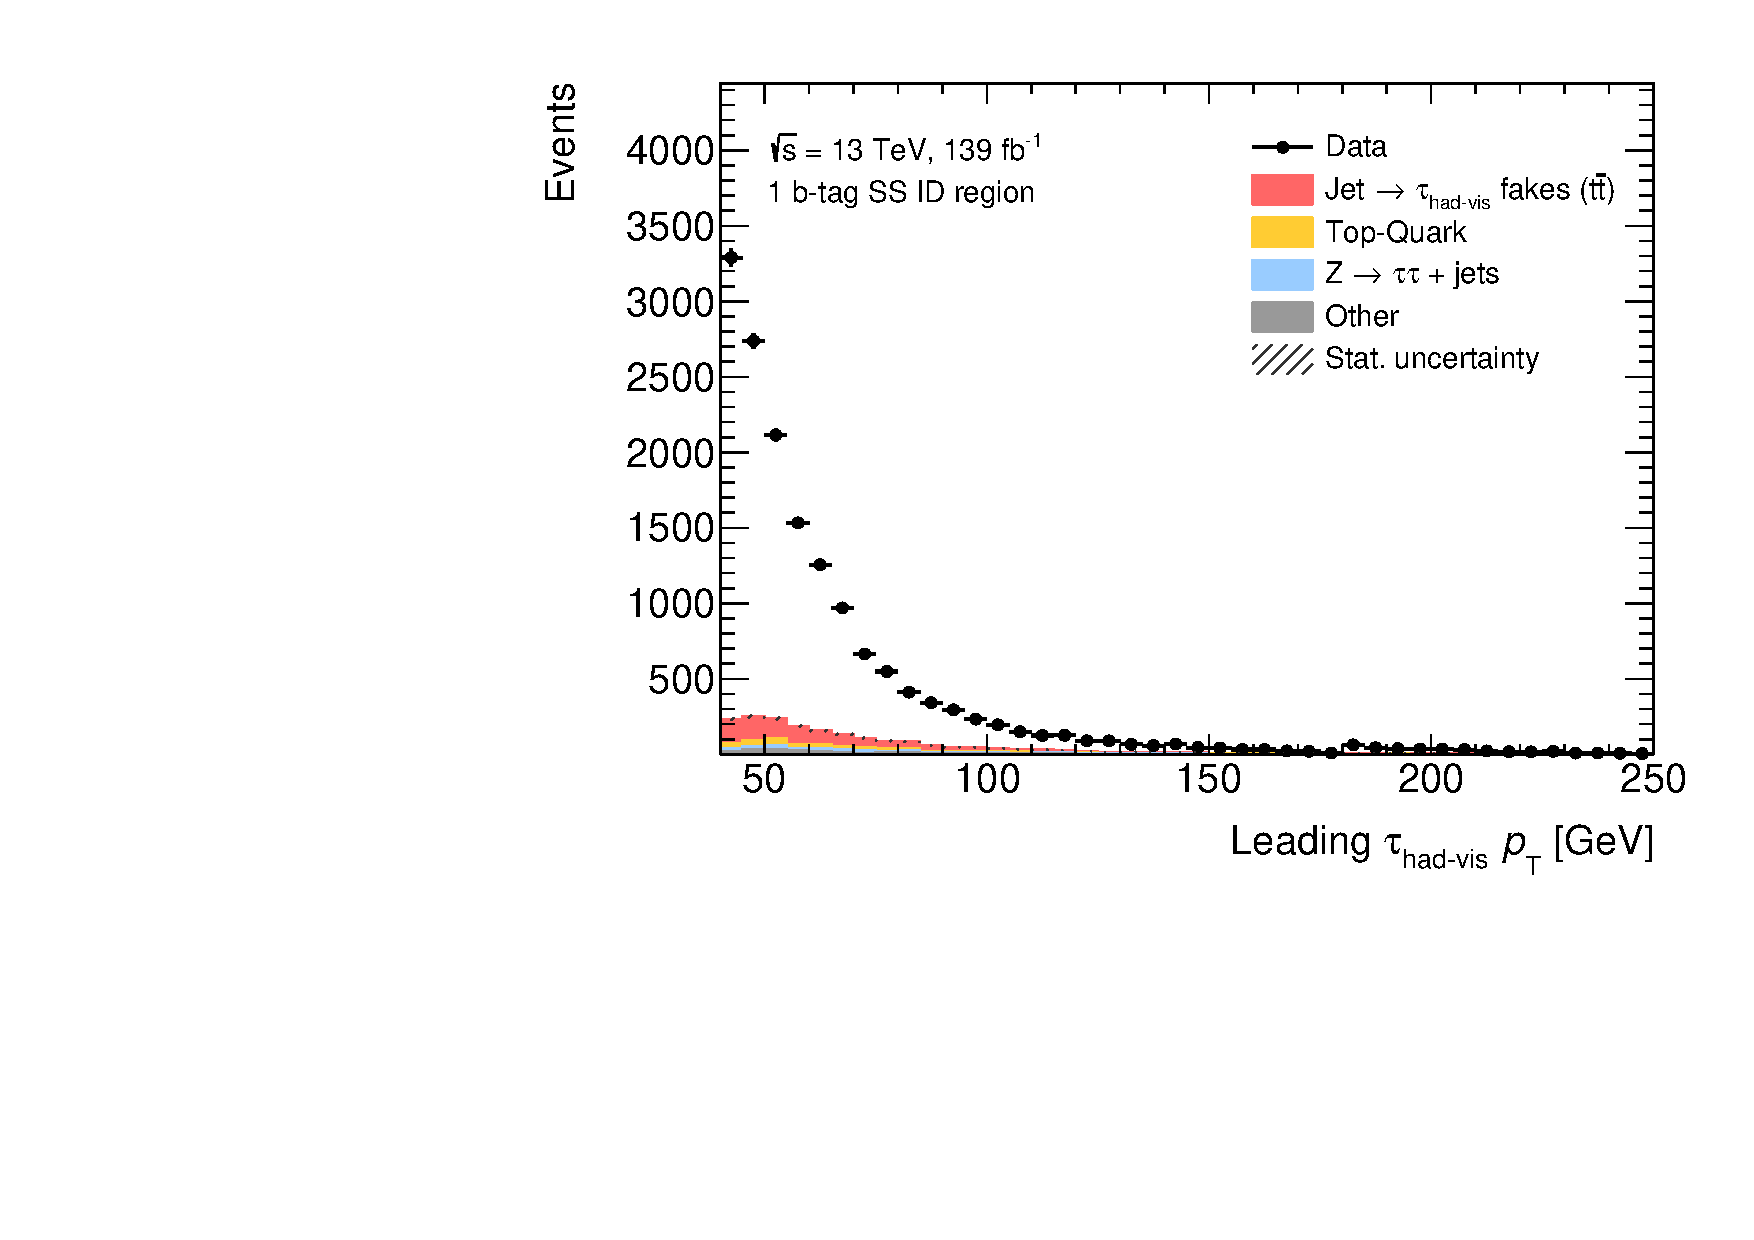
\includegraphics[width=\textwidth]{fakefactors/region_plots/tau0pt_1tag_ss_id}
    \subcaption{1 $b$-tag SS ID region}
  \end{subfigure}
  \begin{subfigure}{0.49\textwidth}
    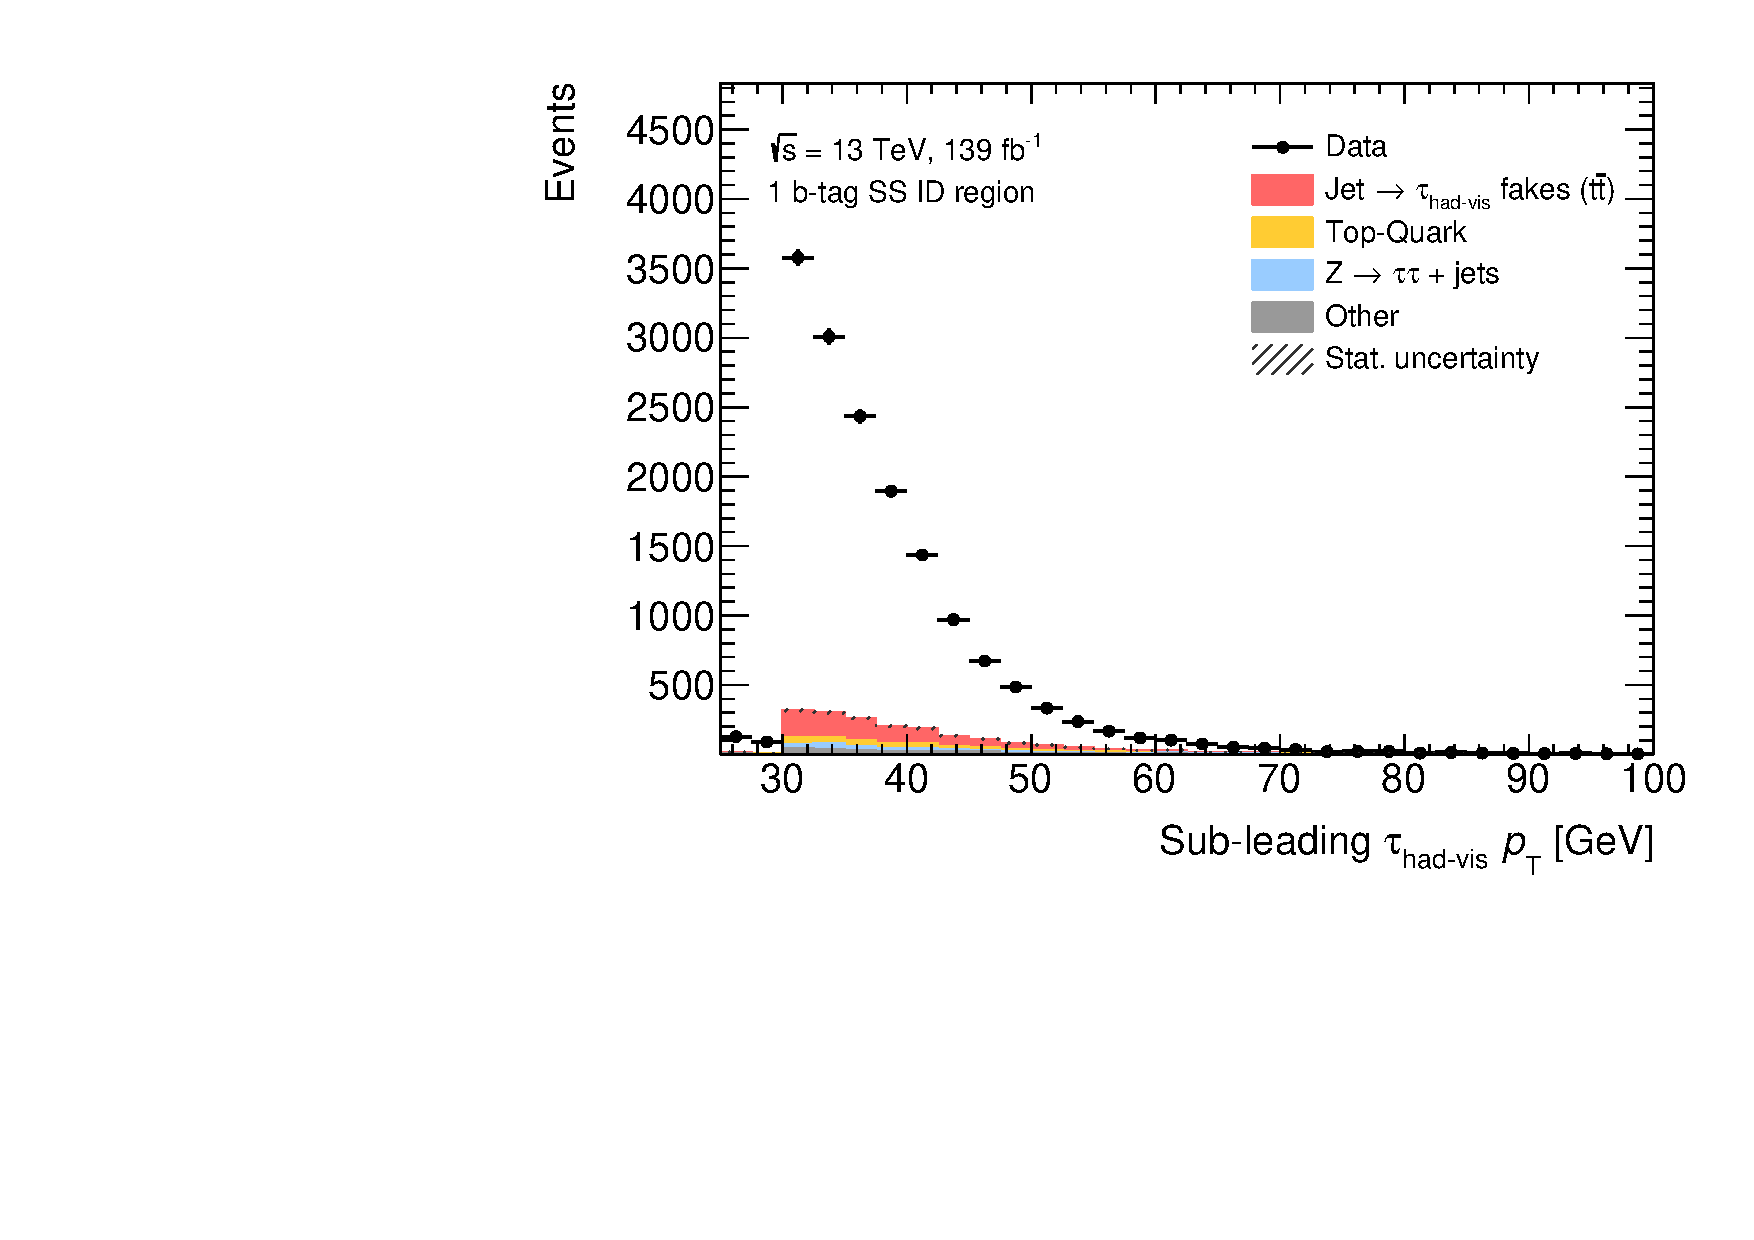
\includegraphics[width=\textwidth]{fakefactors/region_plots/tau1pt_1tag_ss_id}
    \subcaption{1 $b$-tag SS ID region}
  \end{subfigure}

  \begin{subfigure}{0.49\textwidth}
    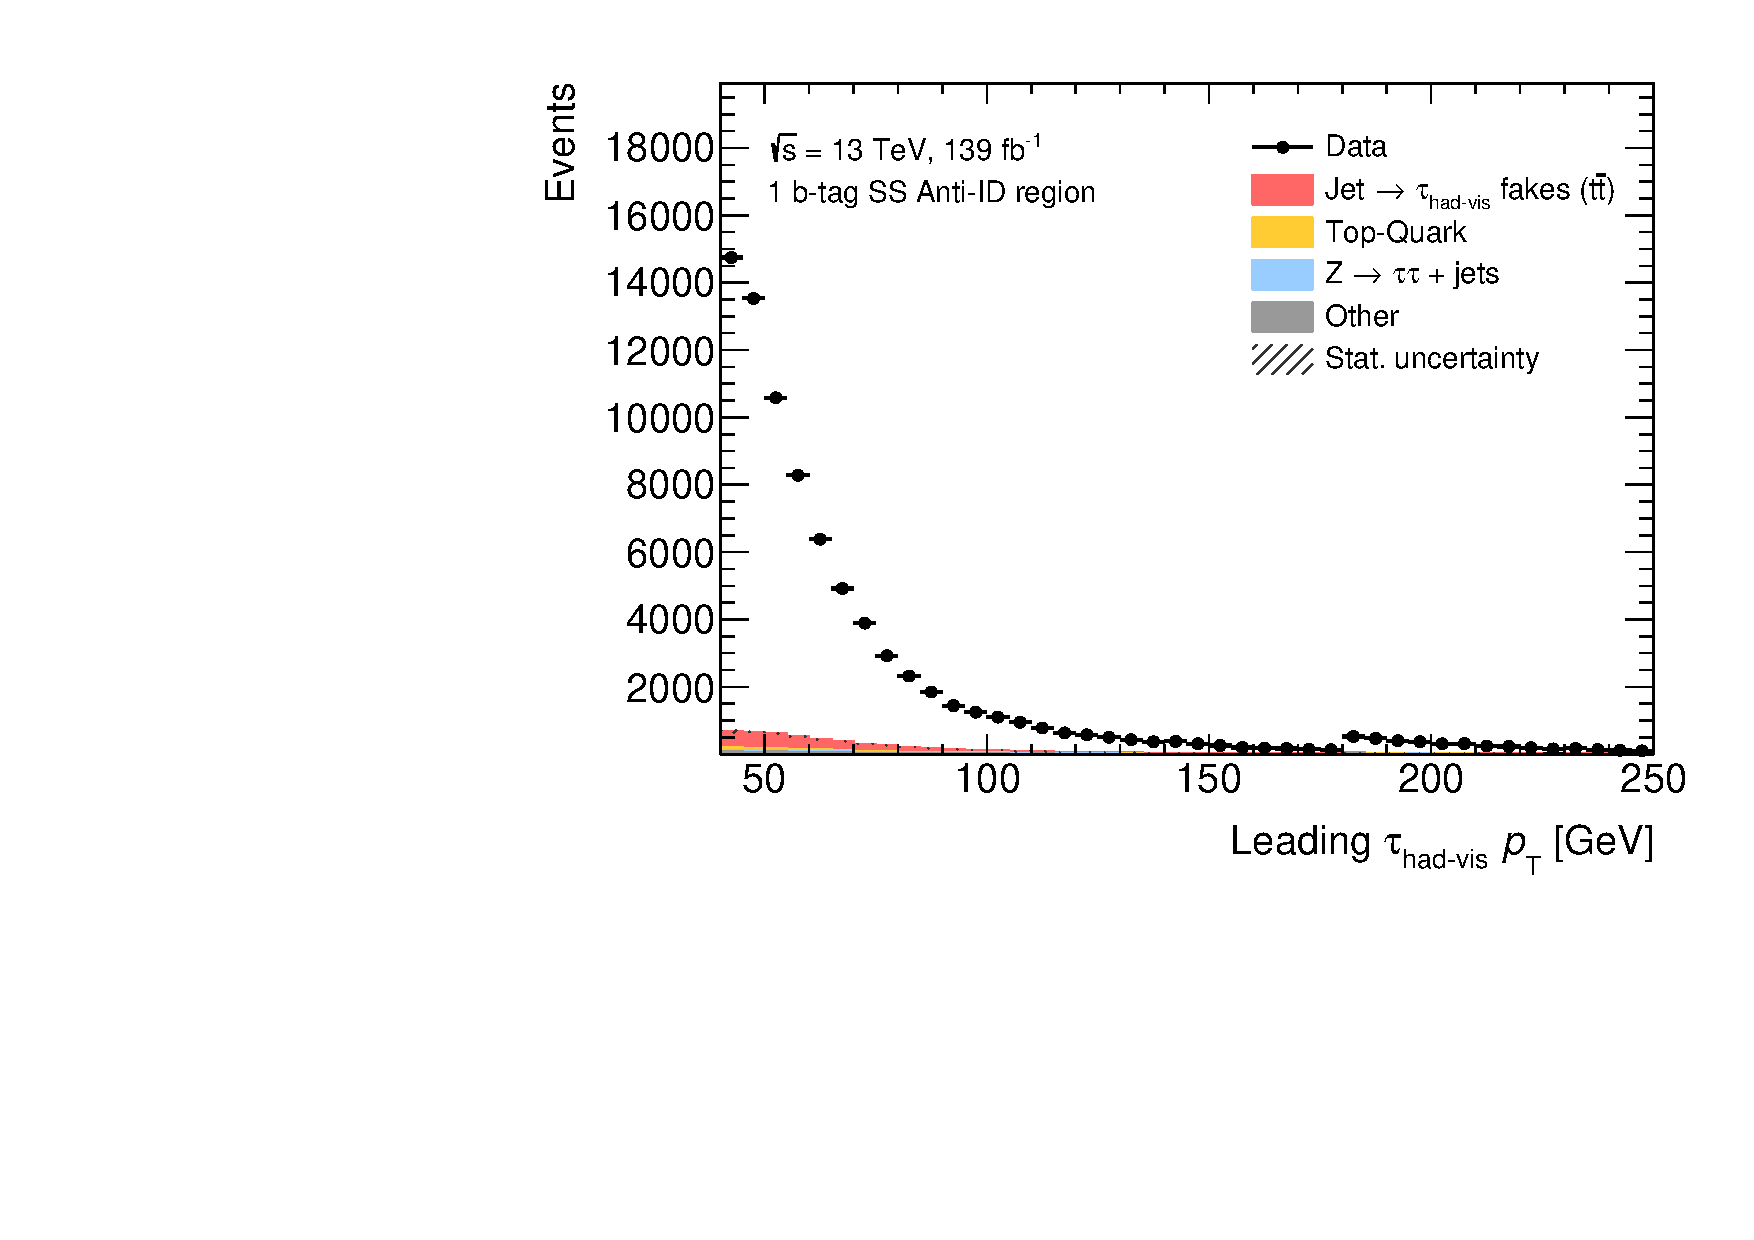
\includegraphics[width=\textwidth]{fakefactors/region_plots/tau0pt_1tag_ss_antiid}
    \subcaption{1 $b$-tag SS Anti-ID region}
  \end{subfigure}
  \begin{subfigure}{0.49\textwidth}
    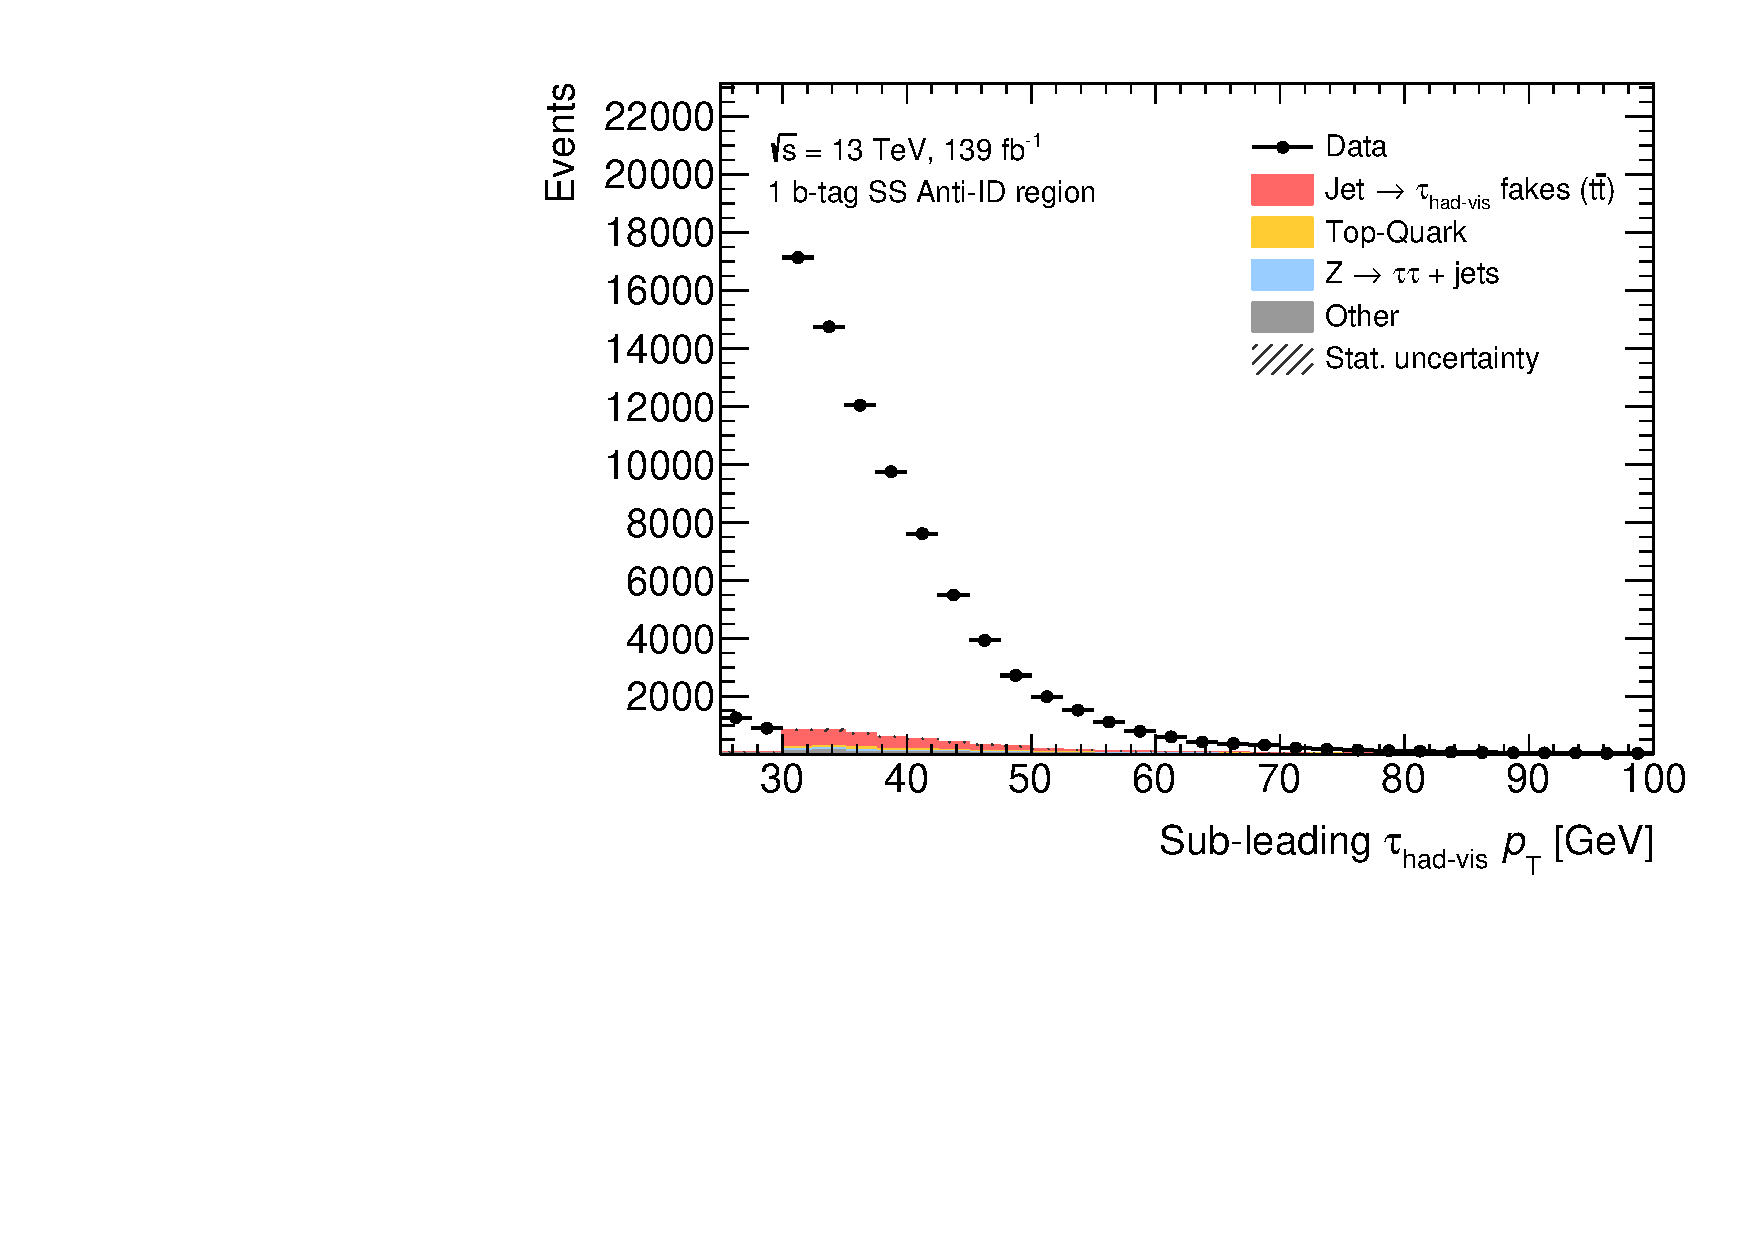
\includegraphics[width=\textwidth]{fakefactors/region_plots/tau1pt_1tag_ss_antiid}
    \subcaption{1 $b$-tag SS Anti-ID region}
  \end{subfigure}

  \caption{Leading (a,c) and sub-leading \tauhadvis \pT (b,d) in
    regions entering the fake factor measurement. The 1 $b$-tag SS ID
    region is shown in (a,b) and the 1 $b$-tag Anti-ID region in
    (c,d). Coloured histograms are contributions from non-multi-jet
    processes (shown with statistical uncertainties only) that are
    subtracted during the measurement. All regions are shown
    inclusively at pre-selection level corresponding to the SS region
    yields and multi-jet purities in \Cref{tab:mjfakes_yields_1tag}.}
  \label{fig:mjfakes_1tag_ss_plots}
\end{figure}

A schematic illustration of this approach is given
in~\Cref{fig:fakefactor_regions}. Fake factors measured in the 1
$b$-tag regions ($\text{FF}_\text{SS}^\text{1-tag}$) are applied to
events in the 2 $b$-tag OS Anti-ID region after subtraction of
non-multi-jet contributions to obtain multi-jet templates in the
signal region. Multiplicative transfer factors
($\text{TF}_{1 \ra 2\,b\text{-tag}}$) are applied to
$\text{FF}_\text{SS}^\text{1-tag}$ when used in 2 $b$-tag regions,
absorbing possible differences between fake factors measured in 1 and
2 $b$-tag regions and the uncertainties associated with this
extrapolation.

\begin{figure}[htbp]
  \centering

  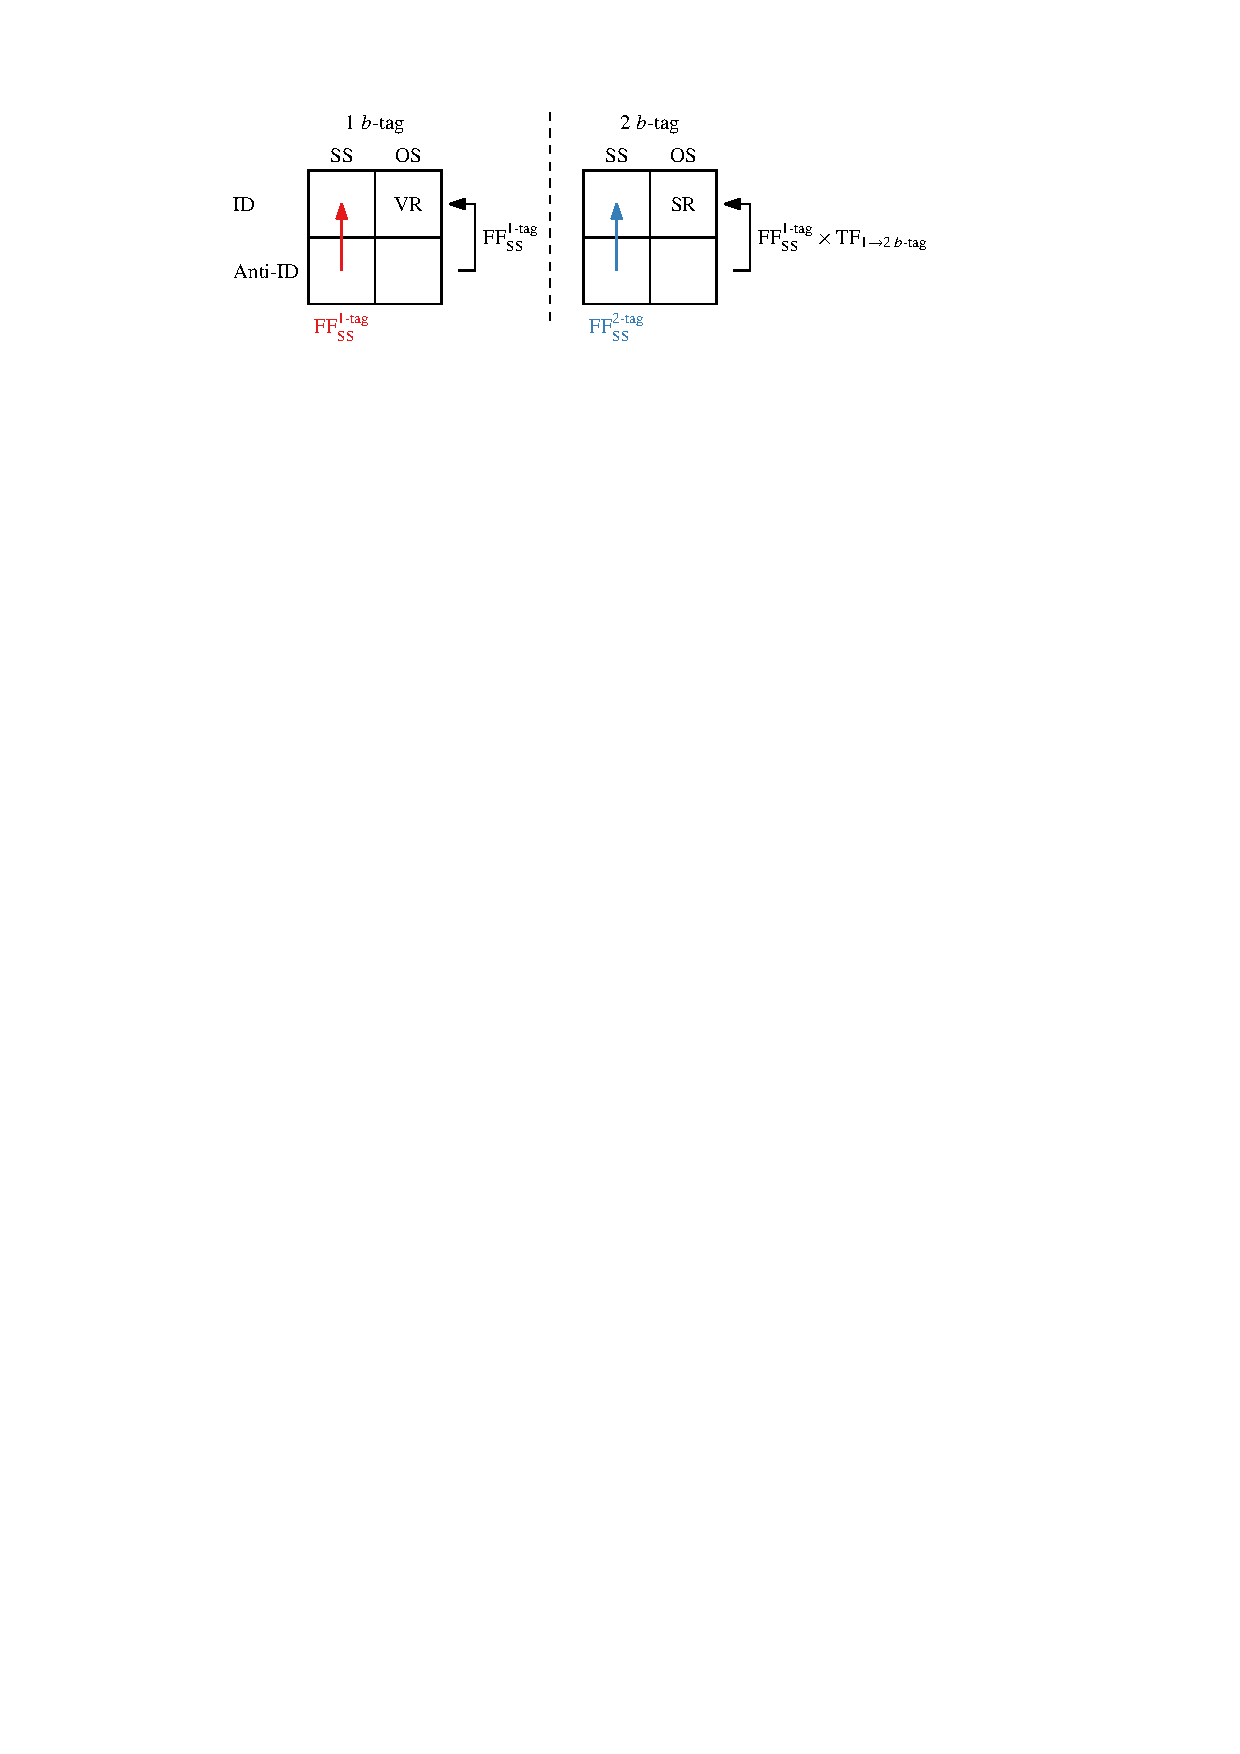
\includegraphics[scale=1]{fakefactors/regions}

  \caption{Schematic description of the fake factor method employed to
    estimate the multi-jet background in the signal region of the
    \hadhad channel. The squares represent the multi-jet events
    ($N_\text{multi-jet} = N_\text{data} - N_\text{non-multi-jet}$) in
    a particular region.}
  \label{fig:fakefactor_regions}
\end{figure}

The 1 $b$-tag OS ID region serves as a validation region to check the
agreement of the total background prediction with the observed data.
% verify the independence of the observables related to \tauid and
% electric charge of the \tauhadvis pair.
This approach is equivalent\todo{Is it really? I
  don't think so.} to a comparison of fake factors measured in the OS
and SS regions\footnote{\Cref{tab:mjfakes_yields_1tag} can be used to
  calculate inclusive fake factors in the OS and SS regions, yielding
  $\text{FF}_\text{SS}^\text{1-tag} \approx
  \text{FF}_\text{OS}^\text{1-tag} \approx 0.18$, which is a
  sufficient condition for statistical independence of the fake factor
  observables at the level of the inclusive selection.}, which have to
agree under the assumptions of the method.\todo{Needs some work...}


\subsubsection{Measurement of fake factors}

% Binning in years / trigger
The fake factor measurement is performed separately for events
selected by single- and di-\tauhadvis triggers as well as the years of
data collection. During Run~2 of the LHC, different \tauhadvis trigger
chains were used by the ATLAS experiment to collect the data used in
this analysis. As a result, the topologies of the selected events and
the \tauid applied at the high-level trigger (HLT) changed as Run~2
progressed. To account for possible differences resulting from the
change in trigger-selection, the fake factor measurement is subdivided
into three major data collection periods: 2015-2016, 2017, and
2018. % The 1 $b$-tag SS regions relevant to the measurement of fake
% factors are shown in~\Cref{fig:mjfakes_1tag_ss_plots}.

% Reason for binning in
The categorisation of the fake factors by trigger that selected the
event is further motivated by the differences between single- and
di-\tauhadvis triggers. Single-\tauhadvis triggers require one
\tauhadvis candidate with high transverse momentum that is identified
at the HLT without any selections applied to the other candidate. In
contrast, di-\tauhadvis triggers require both \tauhadvis to be
identified at the HLT with similar transverse momentum thresholds
applied to both. This allows \tauhadvis candidates in in the
di-\tauhadvis trigger category to be treated equally once
\pT-threshold effects are accounted for. This is not the case in
events selected by single-\tauhadvis triggers.

Dependencies of the fake factors on reconstructed quantities of
\tauhadvis candidates are accounted for by further categorisation
based on the \tauhadvis that distinguishes the ID from the Anti-ID
regions. The fake factor measurement is performed separately for 1-
and 3-prong \tauhadvis candidates, independently of the trigger
category.

Fake factors for events selected by di-\tauhadvis triggers are
additionally measured in dependence of \tauhadvis \pT and separately
for \tauhadvis in the barrel and endcap regions of the ATLAS
detector. In contrast, few multi-jet events enter the
single-\tauhadvis trigger category due to stringent \pT requirements,
thus not allowing a large number of subdivisions for the
measurement. Therefore, the fake factors for singe-\tauhadvis trigger
events are measured separately for cases where the anti-\tauhadvis is
leading and the sub-leading in \pT, accounting for the differences in
HLT \tauid and (typically) large \tauhadvis \pT differences between
both candidates.


\subsubsection{Measurement of fake factors: di-\tauhadvis triggers}

{% Group for extra definitions
  \newcommand*{\ffargs}{\ensuremath{( \myvec{x}_{\tau} )}\xspace}

  \newcommand*{\NmjID}[2]{\ensuremath{N_\text{multi-jet}^{\text{#1, loose }\tau_{#2}}}\xspace}
  \newcommand*{\NmjIDIncl}[1]{\ensuremath{N_\text{multi-jet}^{\text{#1, ID}}}\xspace}

  \newcommand*{\NmjAntiIDIncl}[1]{\ensuremath{N_\text{multi-jet}^{\text{#1, Anti-ID}}}\xspace}
  \newcommand*{\NmjAntiID}[2]{\ensuremath{N_\text{multi-jet}^{\text{#1, anti-}\tau_{#2}}}\xspace}

  The Anti-ID region can be partitioned into two regions differing in
  whether the \tauhadvis candidate leading or sub-leading in \pT is
  reconstructed as the anti-\tauhadvis. Provided the conditions for
  the fake factor method are fulfilled, both regions can be used to
  obtain individual estimates of the multi-jet background in the OS ID
  region. The notation used to describe the fake factor measurement is
  introduced in the following:
  \begin{description}[style=standard]
  \item[$\tau_0$ ($\tau_1$)] The \tauhadvis candidate leading (sub-leading) in \pT.

  \item[$\myvec{x}_\tau$] Categorical observables of a \tauhadvis
    candidate that define the bin of the fake factor measurement. The
    observables used for the di-\tauhadvis trigger fake factors are
    the reconstructed decay mode ($N_\text{tracks}$), the bin of
    \tauhadvis \pT, and the bin of \tauhadvis $\eta$.

  \item[$\NmjID{SS(OS)}{i}\ffargs$] Number of multi-jet events in the
    SS (OS) ID region where~$\tau_i$ has
    observables~$\myvec{x}_\tau$. \todo{Maybe distinguish better from
      the FF estimate?}

  \item[$\NmjAntiID{SS(OS)}{i}\ffargs$] Number of multi-jet events in
    the SS (OS) Anti-ID region where $\tau_i$ is the anti-\tauhadvis
    with observables~$\myvec{x}_\tau$.
  \end{description}
  With these definitions, two sets of fake factors can be defined as
  \begin{align*}
    \FF_{i}\ffargs &= \frac{\NmjID{SS}{i} \ffargs}{\NmjAntiID{SS}{i}\ffargs}
                     \quad \text{for} \quad i = 0, 1 \,\text{,}
  \end{align*}
  where $\FF_{i}$ is the fake factor relating the ID region with the
  partition of the Anti-ID region where $\tau_i$ is the
  anti-\tauhadvis. These can be used to obtain two multi-jet estimates
  in the OS region given by
  \begin{align*}
    \NmjID{OS}{i}\ffargs = \FF_{i}\ffargs \cdot \NmjAntiID{OS}{i}\ffargs
    \quad \text{for} \quad i = 0, 1 \,\text{.}
  \end{align*}
  An average of both estimates can be calculated, yielding fake
  factors that are inclusive in whether the anti-\tauhadvis is the
  leading or sub-leading \tauhadvis candidate. The inclusive fake
  factors can be expressed as
  \begin{align*}
    \FF_\text{incl.}\ffargs = \frac{1}{2} \left[ f_0\ffargs \cdot \FF_0\ffargs
    + f_1\ffargs \cdot \FF_1\ffargs \right] \,\text{,}
  \end{align*}
  with $f_i\ffargs$ being the fraction of Anti-ID events where
  $\tau_i$ is the anti-\tauhadvis and has
  observables~$\myvec{x}_\tau$. The inclusive fake factor can be
  measured directly according to
  \begin{align}
    \FF_\text{incl.}\ffargs
    = \frac{1}{2} \frac{ \NmjID{SS}{0}\ffargs + \NmjID{SS}{1}\ffargs }
                       { \NmjAntiID{SS}{0}\ffargs + \NmjAntiID{SS}{1}\ffargs }
    \label{eq:inclusive_fake_factor}
  \end{align}
  and the multi-jet estimate in the OS region obtained by
  \begin{align*}
    \NmjIDIncl{OS}\ffargs = \FF_\text{incl.}\ffargs \cdot \NmjAntiIDIncl{OS}\ffargs \,\text{,}
  \end{align*}
  where $\NmjAntiIDIncl{OS}\ffargs$ is the number of multi-jet events
  in the OS Anti-ID region\todo{Emphasise that this is now the
    inclusive region?} with anti-\tauhadvis $\myvec{x}_\tau$.

  % Prior the agreement of the background estimates obtained with FF0
  % and FF1 were confirmed.

  The motivation of using inclusive fake factors is two-fold. First,
  it allows to use all events entering the Anti-ID region, independent
  of whether the anti-\tauhadvis is leading or sub-leading in \pT,
  thus improving the statistical precision of the background
  estimate. Second, the fake factors can be parametrised in the
  properties of the anti-\tauhadvis directly, allowing to target the
  key differences between the ID and Anti-ID regions. This represents
  a change with respect to the previous
  publication~\cite{HIGG-2016-16-witherratum} where fake factors were
  parametrised jointly in the properties of both \tauhadvis
  candidates, thus limiting the statistical precision of the fake
  factor measurement due to high dimensionality\todo{Note that
    previously AA events were considered?}.

}

The inclusive fake factors for events selected by di-\tauhadvis
triggers are measured according to~\Cref{eq:inclusive_fake_factor} and
parametrised in \tauhadvis decay mode, transverse momentum,
pseudorapidity, and the period of data collection. The number of
multi-jet events is obtained by subtracting the expected number of
non-multi-jet events estimated using simulation from the number of
observed events in data. The measured fake factors are summarised
in~\Cref{fig:mjfakes_fake_factors}.

\begin{figure}[htbp]
  \centering

  \begin{subfigure}{0.495\textwidth}
    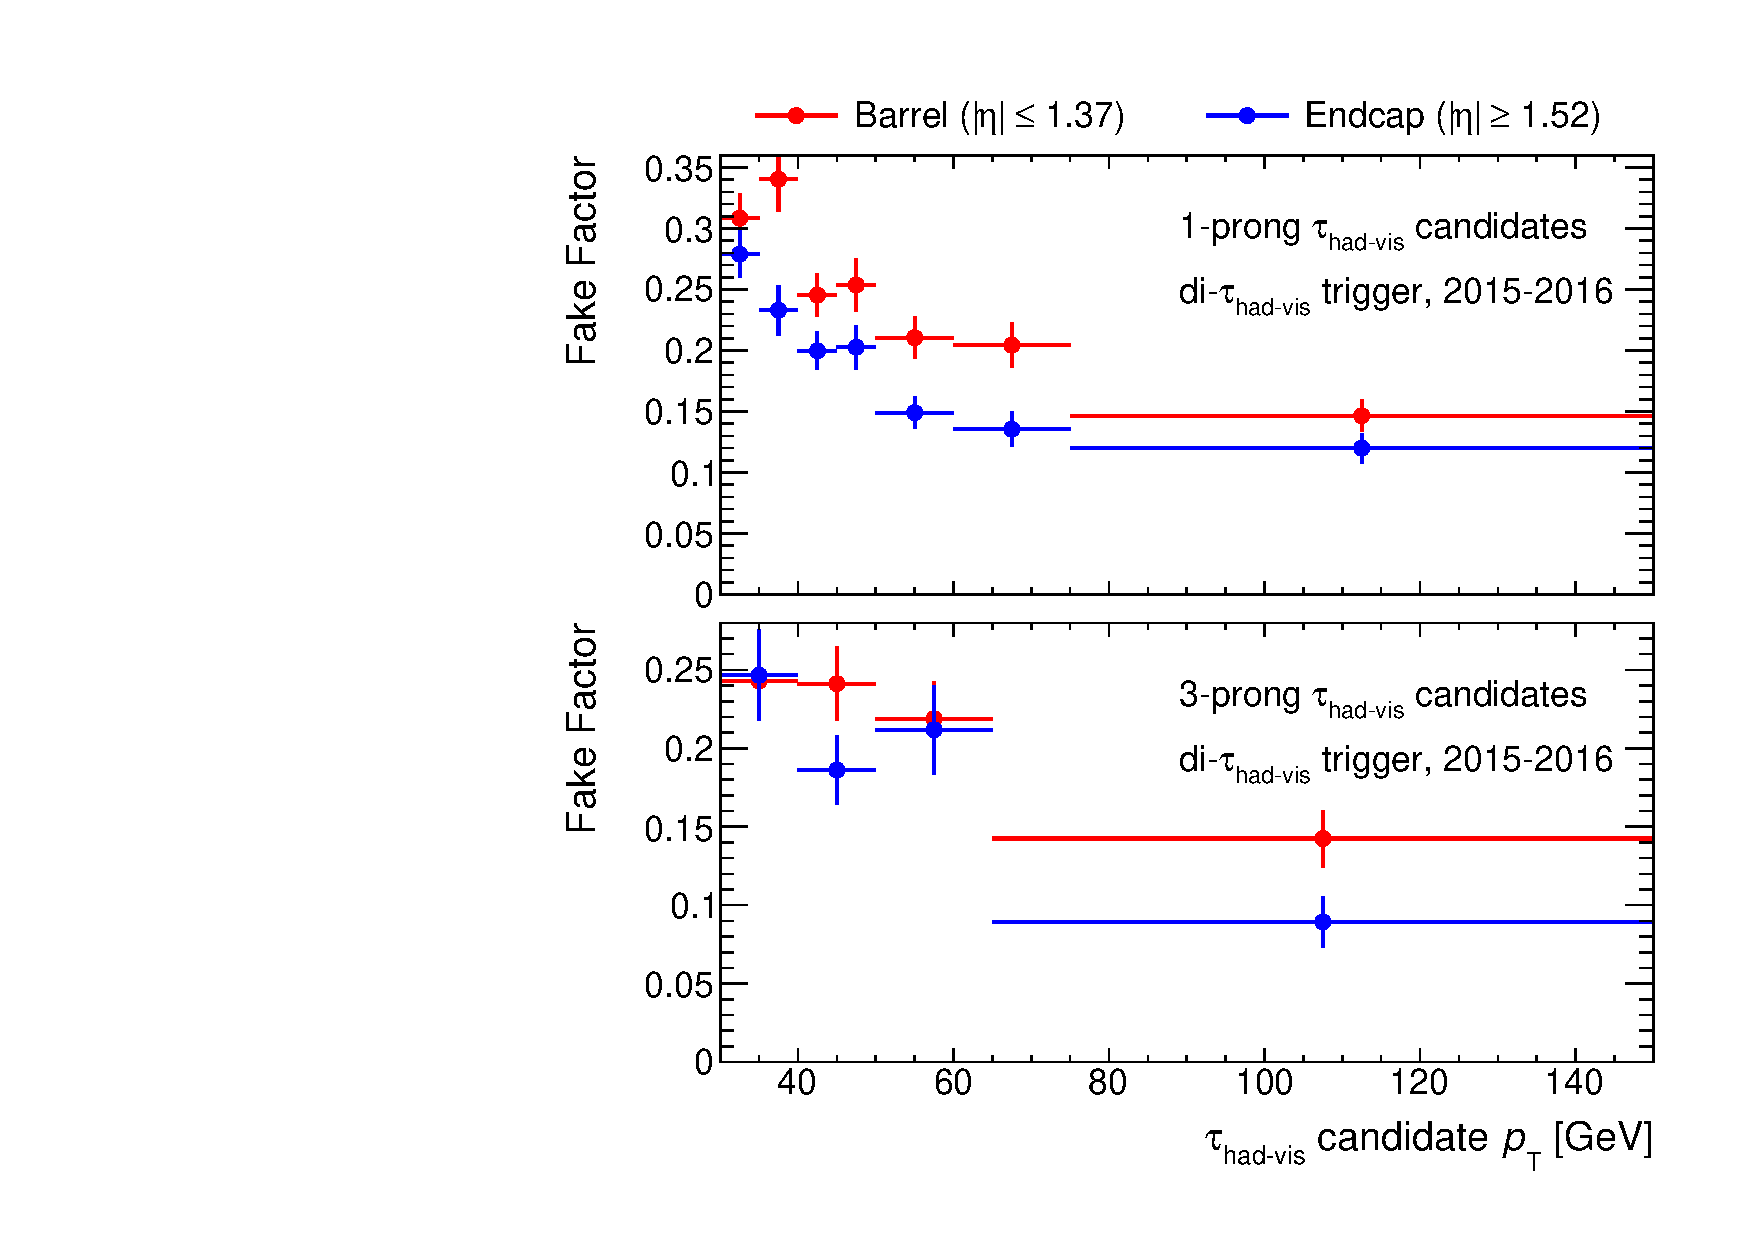
\includegraphics[width=\textwidth]{fakefactors/fake_factors_dtt_1516}
    \subcaption{2015-2016 data collection period}
  \end{subfigure}
  \begin{subfigure}{0.495\textwidth}
    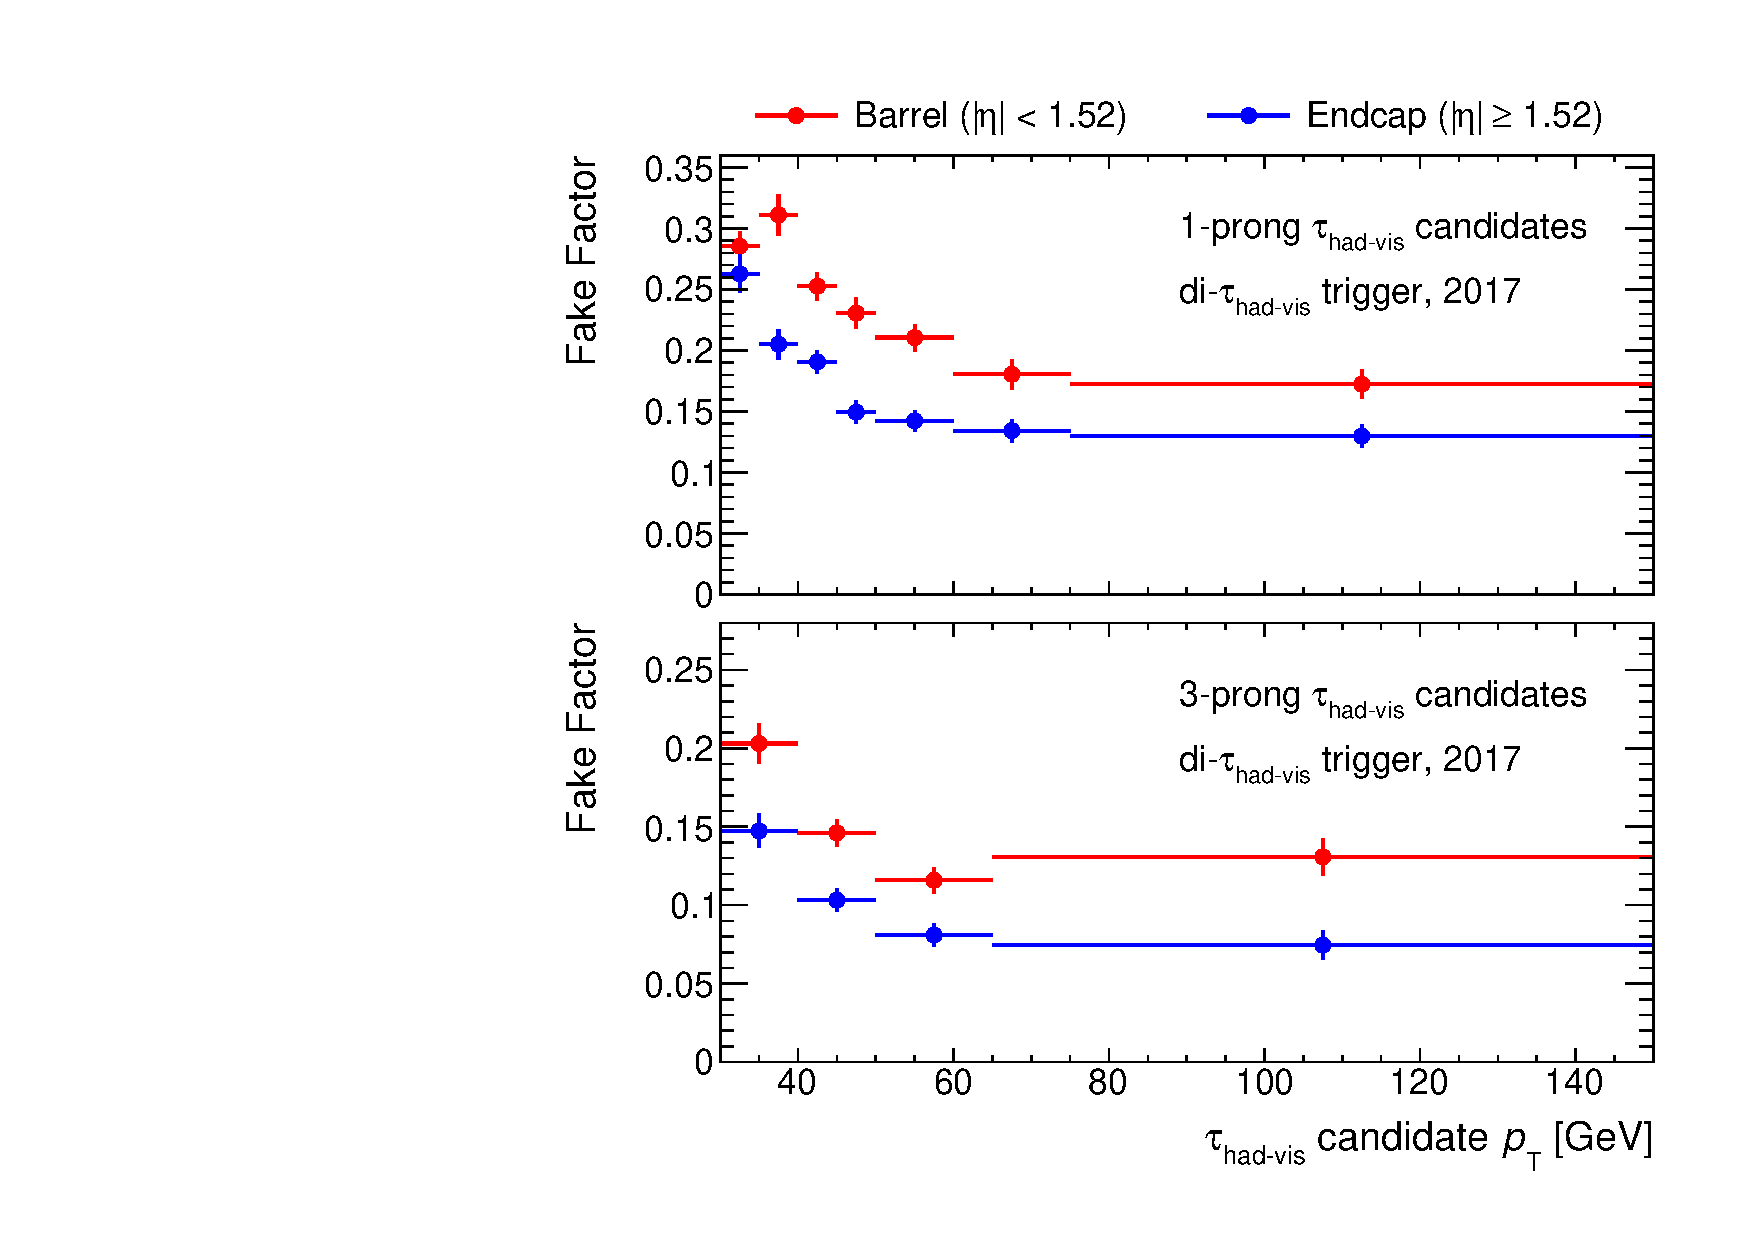
\includegraphics[width=\textwidth]{fakefactors/fake_factors_dtt_17}
    \subcaption{2017 data collection period}
  \end{subfigure}

  \begin{subfigure}{0.495\textwidth}
    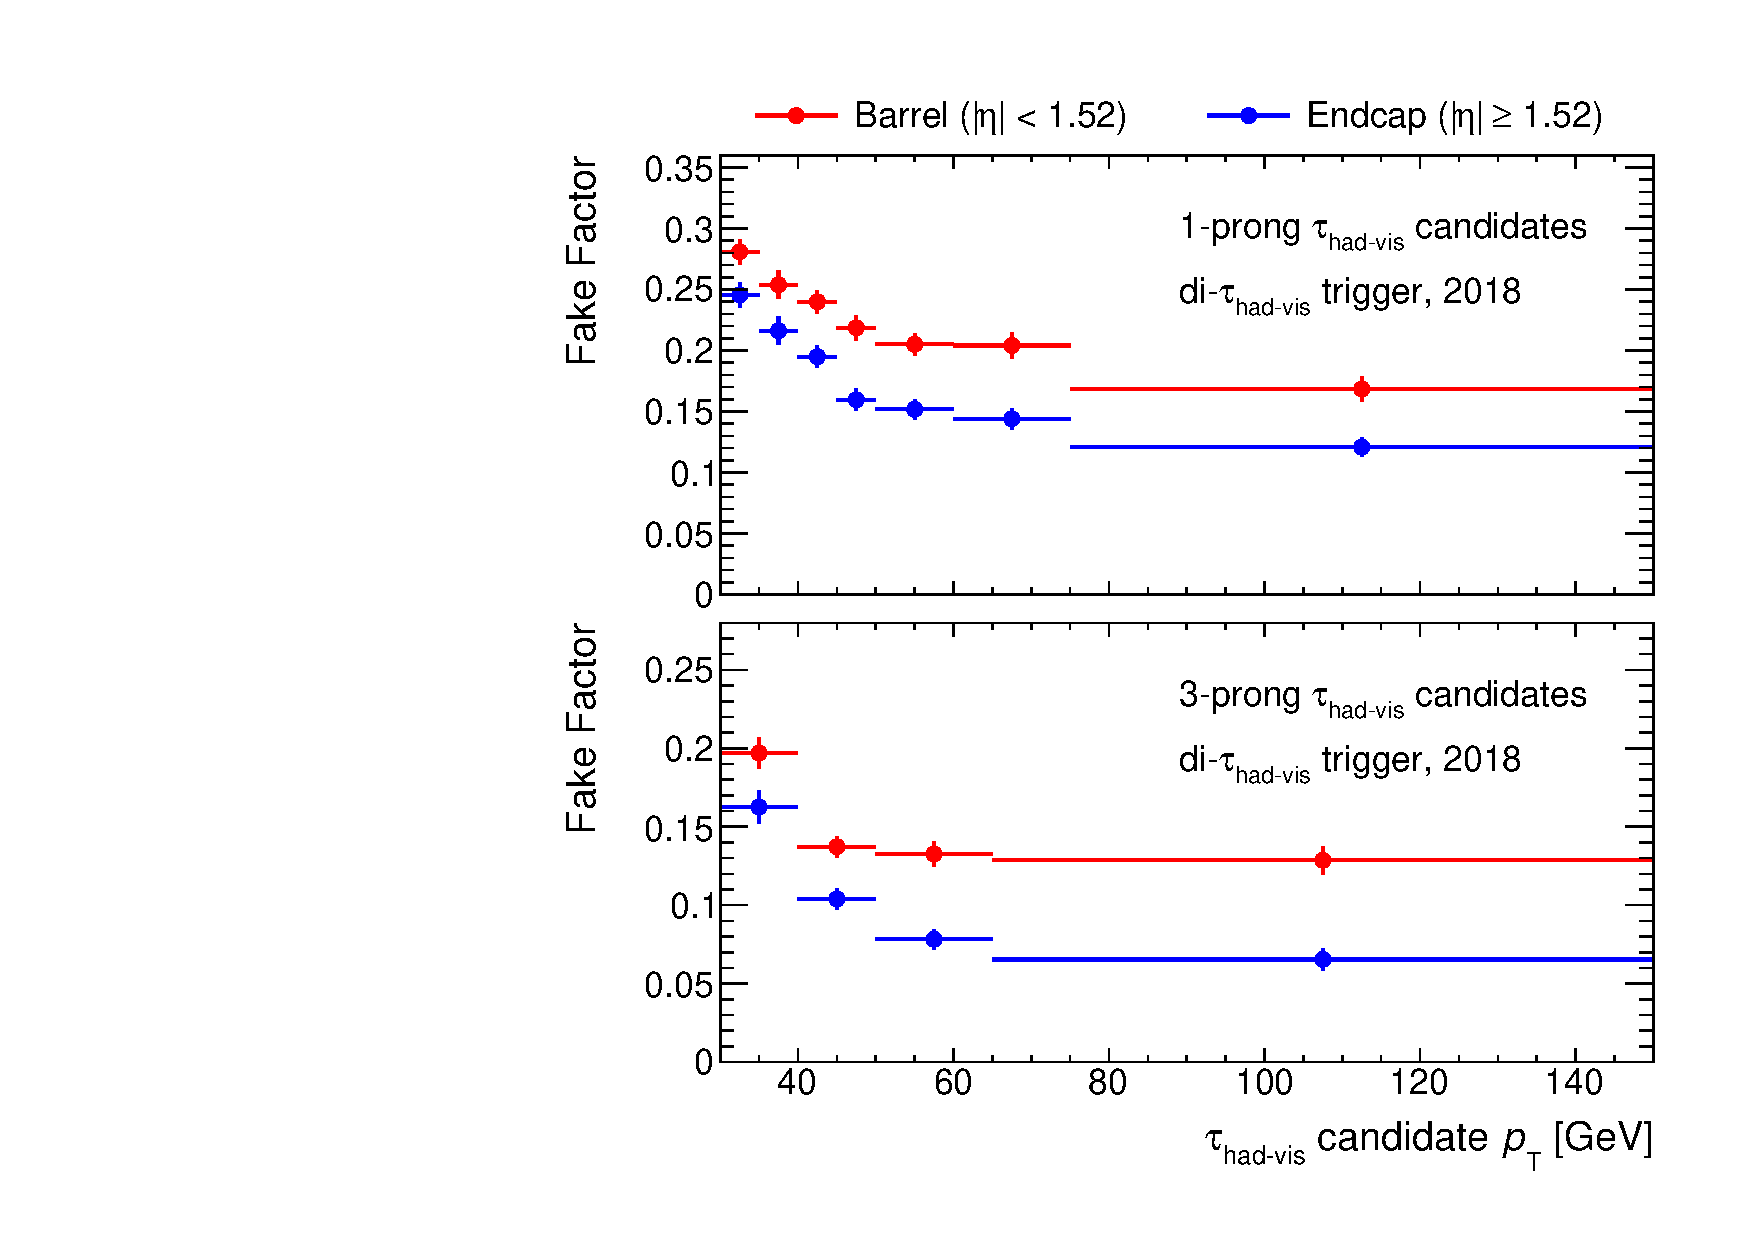
\includegraphics[width=\textwidth]{fakefactors/fake_factors_dtt_18}
    \subcaption{2018 data collection period}
  \end{subfigure}

  \caption{Inclusive fake factors (1 $b$-tag SS) for events selected
    by di-\tauhadvis triggers measured separately for three major data
    collection periods (a-c), 1- and 3-prong \tauhadvis candidates
    (upper and lower panel), and for \tauhadvis in the barrel (red
    markers) and endcap regions (blue markers) of the ATLAS
    detector. Events with (anti-)\tauhadvis $\pT > \SI{150}{\GeV}$ are
    merged into the last fake factor bin. Uncertainties are from
    statistical sources only. Systematic uncertainties originating
    from the non-multi-jet subtraction are assumed to be negligible
    due to the small size of the subtraction.}
  \label{fig:mjfakes_fake_factors}
\end{figure}

Qualitatively, the behaviour of the fake factors with respect to the
\tauhadvis properties is the same between all data collection
periods. Minor differences exist when comparing different periods. No
attempt was made to combine the measurements of certain periods as the
statistical precision of the fake factor measurement is not a limiting
factor in the analysis.


\subsubsection{Measurement of fake factors: single-\tauhadvis triggers}

The measurement of fake factors for events selected by
single-\tauhadvis triggers has to proceed differenty from the
di-\tauhadvis trigger case. First, at the HLT \tauhadvis
identification is only applied to one of the \tauhadvis candidates,
preventing an inclusive treatment of both \tauhadvis
candidates. Second, the high \pT thresholds on \tauhadvis at
trigger-level has high rejection of most SM processes, limiting the
number of events entering the control regions for the fake factor
measurement. As a result, the fake factors for singe-\tauhadvis
triggers cannot be measured differentially in \tauhadvis \pT and
$\eta$.

The STT fake factors are measured in four categories for every major
period of data collection: 1- and 3-prong \tauhadvis and whether the
\tauhadvis is leading or sub-leading in \pT. The resulting fake
factors are summarised in~\Cref{fig:mjfakes_stt_ffs}.


% Additional info that would be interesting:
% - Subtraction

\begin{figure}[htbp]
  \centering

  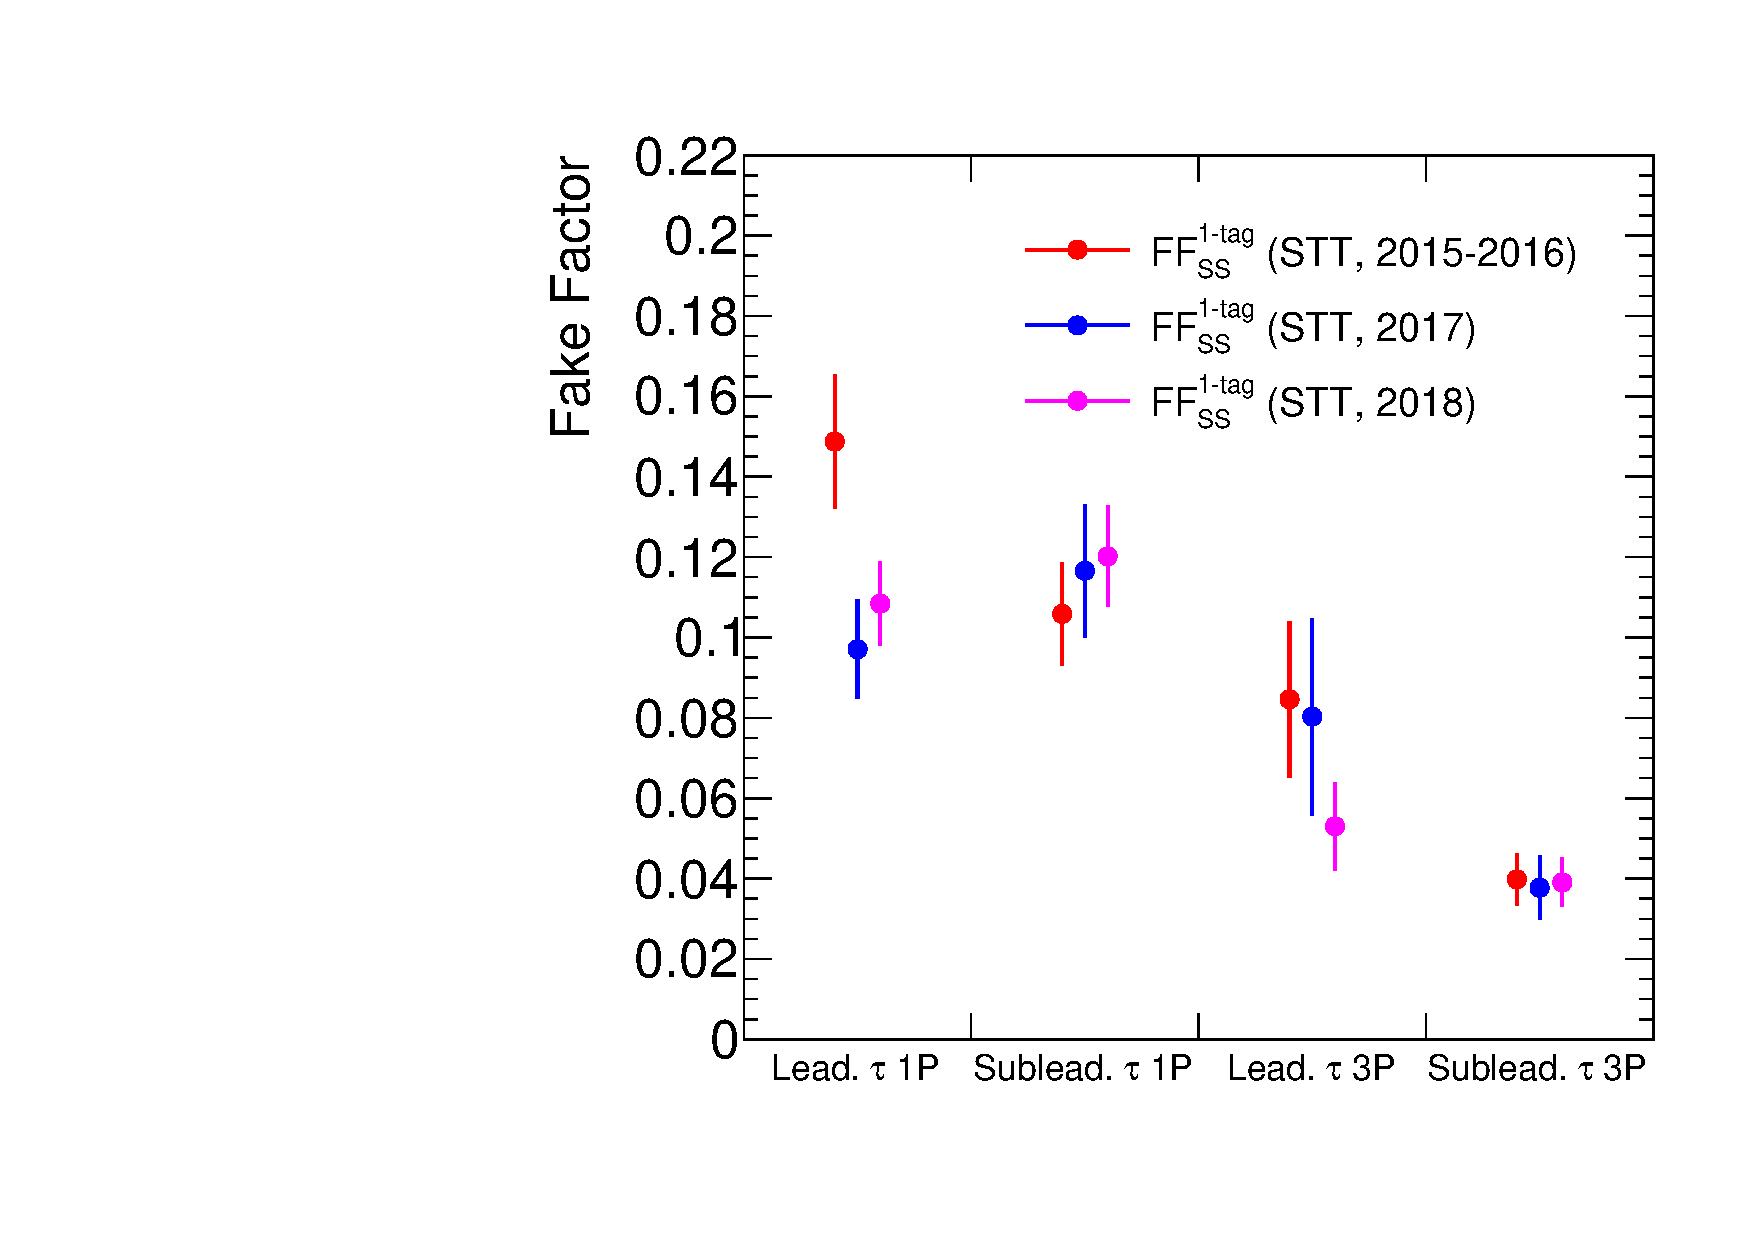
\includegraphics[width=0.495\textwidth]{fakefactors/fake_factors_stt}

  \caption{Fake factors (1 $b$-tag SS) for events selected by
    single-\tauhadvis triggers measured separately for the three major
    data collection periods. The measurement is performed (inclusively
    in \tauhadvis \pT and $\eta$) in bins of the reconstructed
    \tauhadvis decay mode (1- and 3-prong) and separately for cases
    where the \pT leading and sub-leading \tauhadvis is the
    anti-\tauhadvis ($\tau_0$ and $\tau_1$).}%
  \label{fig:mjfakes_stt_ffs}

  \todo[inline]{Largest deviation for leading 1-prong tau possibly due
    to looser pT threshold.}
\end{figure}


\begin{figure}[htbp]
  \centering

  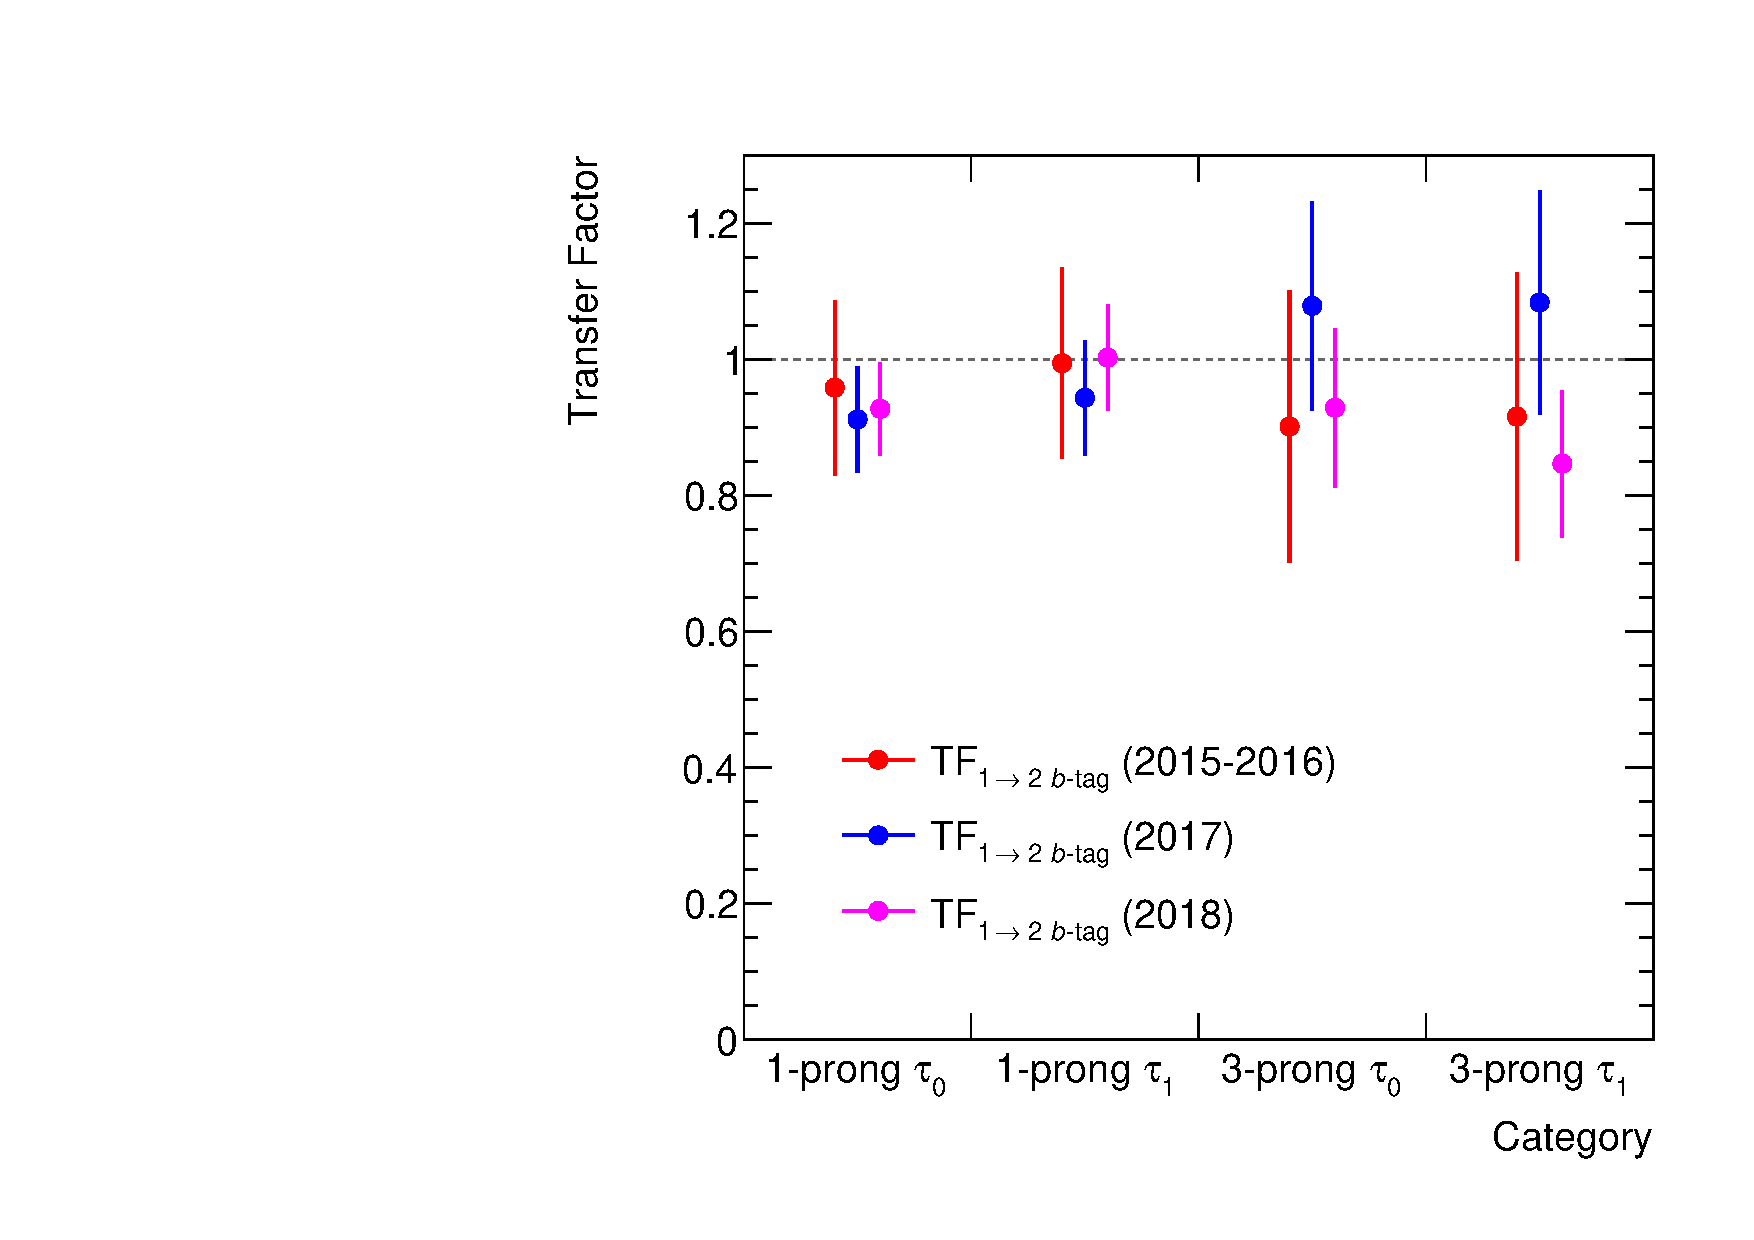
\includegraphics[width=0.495\textwidth]{fakefactors/transfer_factors}

  \caption{Transfer Factors}
  \label{fig:mjfakes_transfer_factor}
\end{figure}


\subsubsection{Estimation of multi-jet backgrounds in the signal region}

% - Transfer factor calculation
% - Subtraction in Anti-ID region

\subsubsection{Validation of the Fake Estimate in 1-tag OS}

An independent validation of the background estimation technique can
be performed in the 1 $b$-tag OS region, which is not part of the fake
factor measurement. At pre-selection level, this region has a
multi-jet purity of about \SI{50}{\percent} with other contributions
from $\Zjets$ and \ttbar. The multi-jet purity can be increased for
validation purposes of the multi-jet background estimate by requiring
% https://twiki.cern.ch/twiki/bin/view/AtlasProtected/MetSignificance
% Using `TreatPUJets == true' and Basic soft term (met::Random)
\begin{align*}
  \mMMC > \SI{110}{\GeV} \qquad \text{and} \qquad \mathcal{S} < 3 \,\text{,}
\end{align*}
where $\mathcal{S}$ is the object-based \pTmissAbs
significance~\cite{ATLAS-CONF-2018-038} that measures the statistical
significance of a test probing the hypothesis of no real \pTmissAbs
compared to the alternative of having real \pTmissAbs. The
contribution of \Zjets is reduced by rejecting events close to the \PZ
boson mass. Multi-jet events are expected to have little real
\pTmissAbs, thus events with significant \pTmissAbs are rejected to
reduce the \ttbar contribution in this
region. In~\Cref{fig:fake_factor_OSVR_cutvars} both variables are
shown in the 1 $b$-tag OS region at pre-selection level to illustrate
this choice of selection for the multi-jet validation region. The
purity of multi-jet validation region is increased to about
\SI{75}{\percent}.

\begin{figure}[htbp]
  \centering

  \begin{subfigure}{0.45\textwidth}
    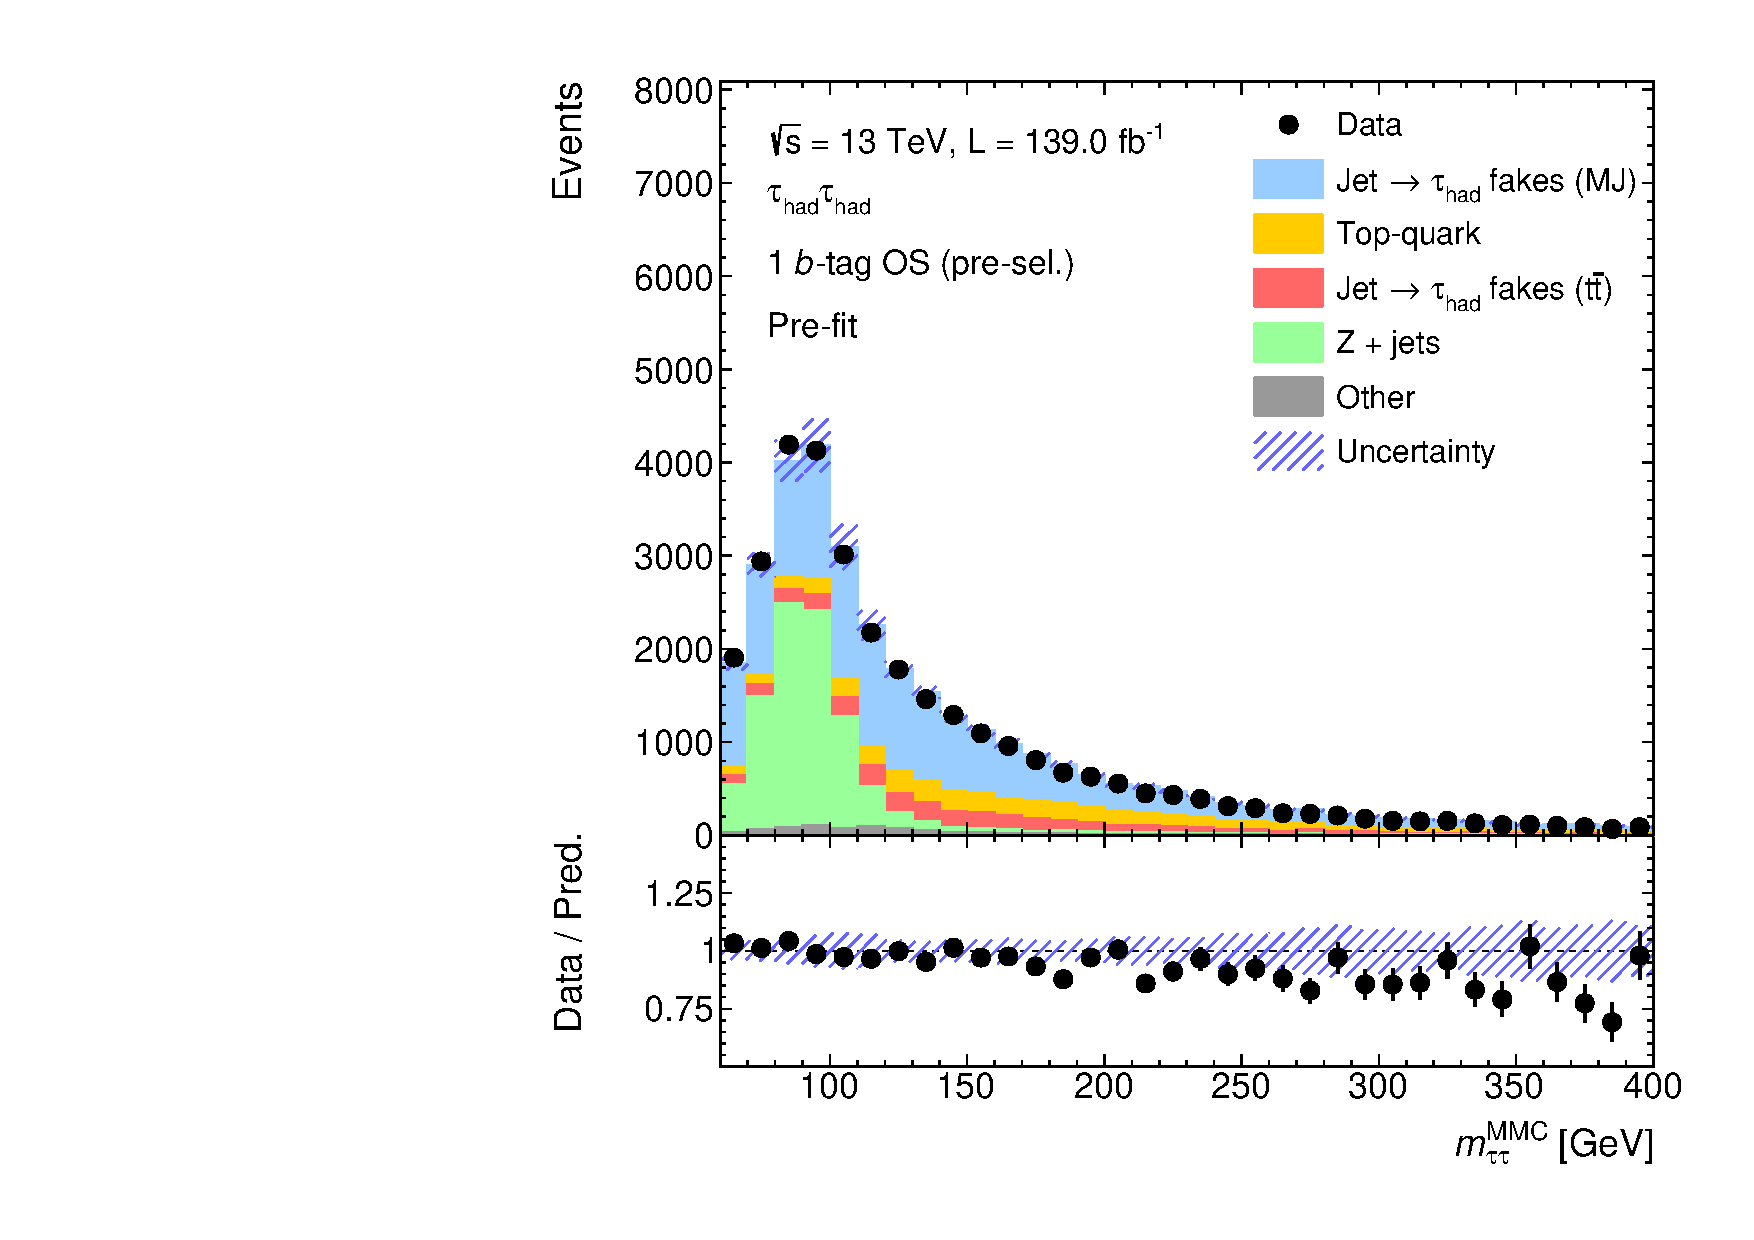
\includegraphics[width=\textwidth]{fakefactors/fake_os_vr/mMMC_presel}
    \subcaption{}
  \end{subfigure}\hspace*{0.04\textwidth}%
  \begin{subfigure}{0.45\textwidth}
    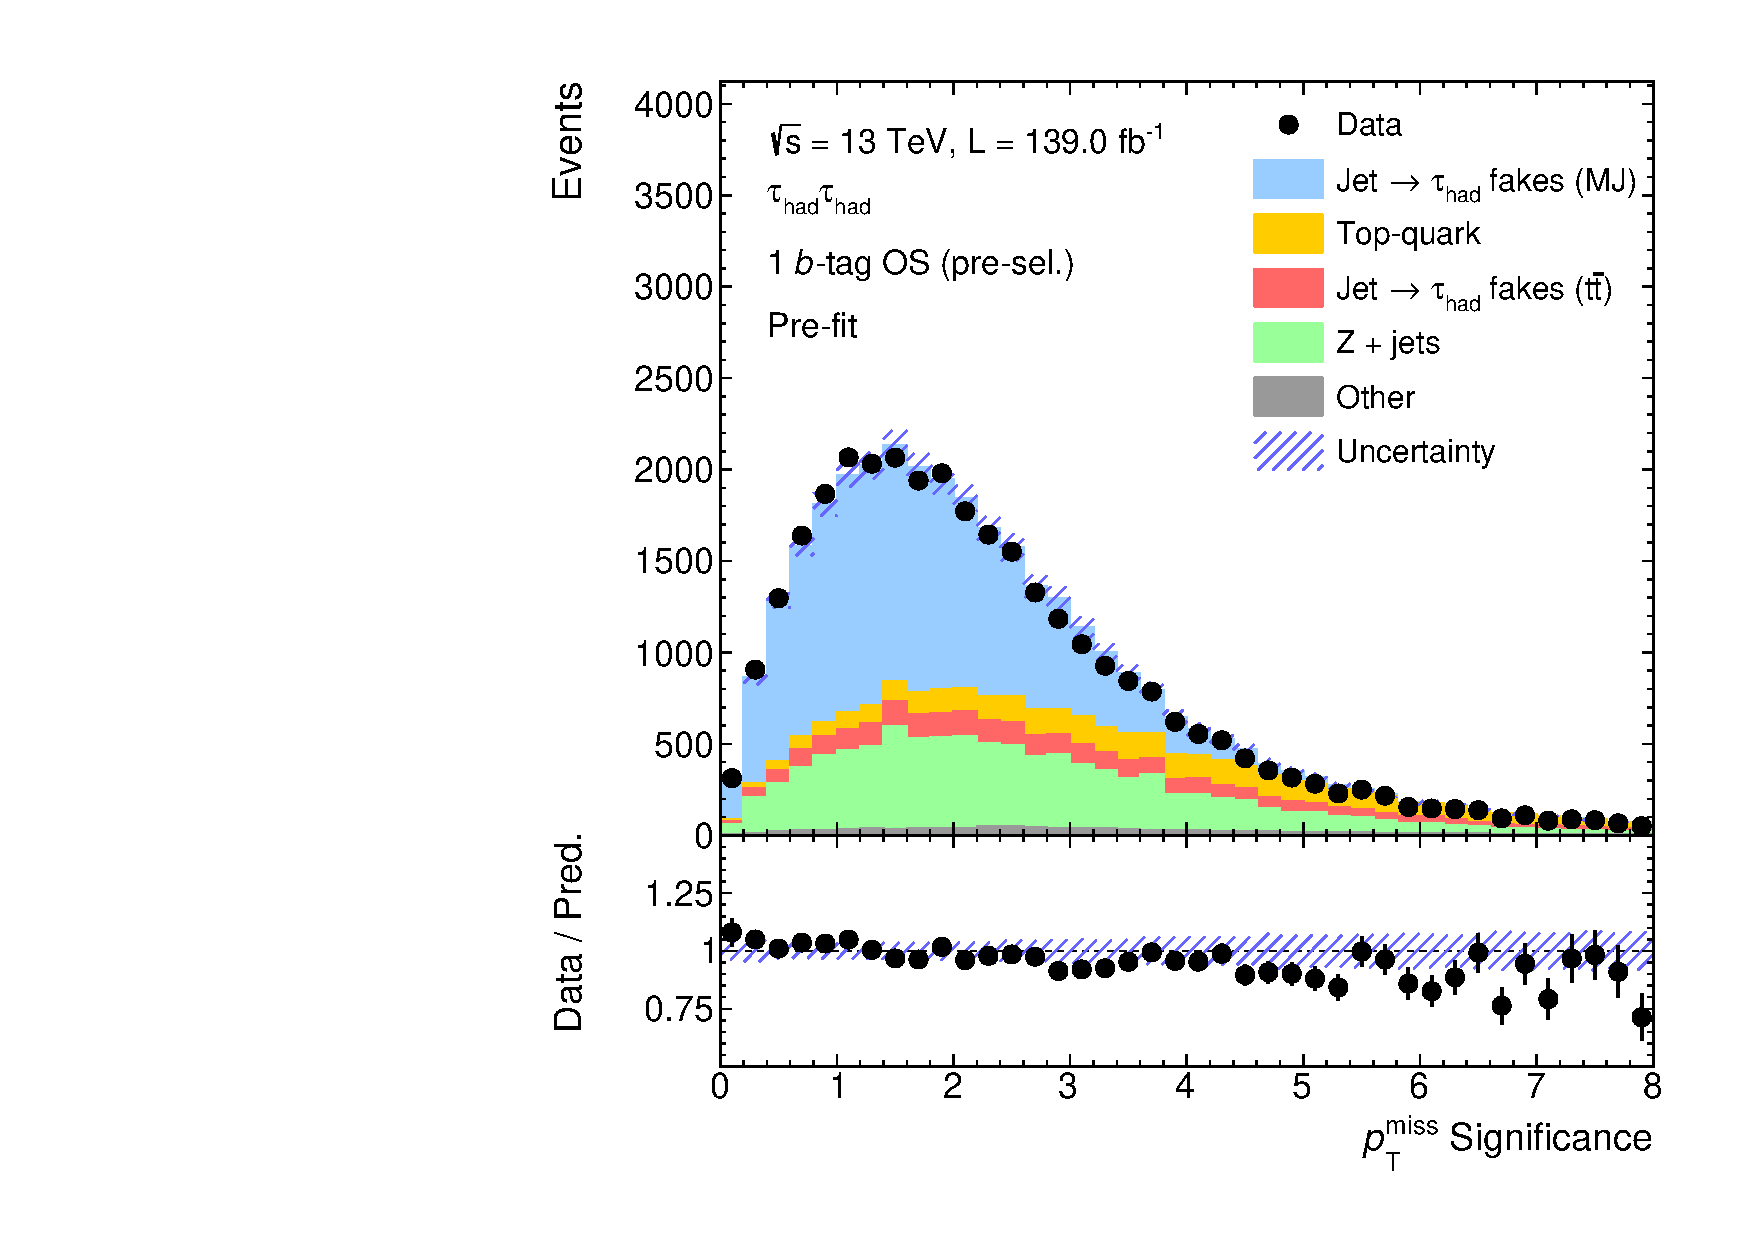
\includegraphics[width=\textwidth]{fakefactors/fake_os_vr/metSig_presel}
    \subcaption{}
  \end{subfigure}

  \caption{The invariant di-\tauhad mass (a) and the object-based
    \pTmissAbs significance (b) in the 1 $b$-tag OS ID region at
    pre-selection level. The estimate of the multi-jet background
    (light blue) is obtained using the fake factor method (cf.\
    \Cref{fig:fakefactor_regions}). Fake-\tauhadvis originating from
    \ttbar (red) are estimated using simulation. The background
    prediction is shown pre-fit, including statistical and
    detector-related systematic uncertainties.}
  \label{fig:fake_factor_OSVR_cutvars}
\end{figure}

The background prediction in the multi-jet validation region is
compared to data in~\Cref{fig:fake_factor_OSVR_kinematics}. The
multi-jet background is estimated using the fake factor method by
applying fake factors measured in the SS regions to events in the OS
Anti-ID region. The background prediction is in good agreement with
the observed data in the validation region, indicating the validity of
the assumptions made by the fake factor method.

\begin{figure}[p]
  \centering

  \begin{subfigure}{0.45\textwidth}
    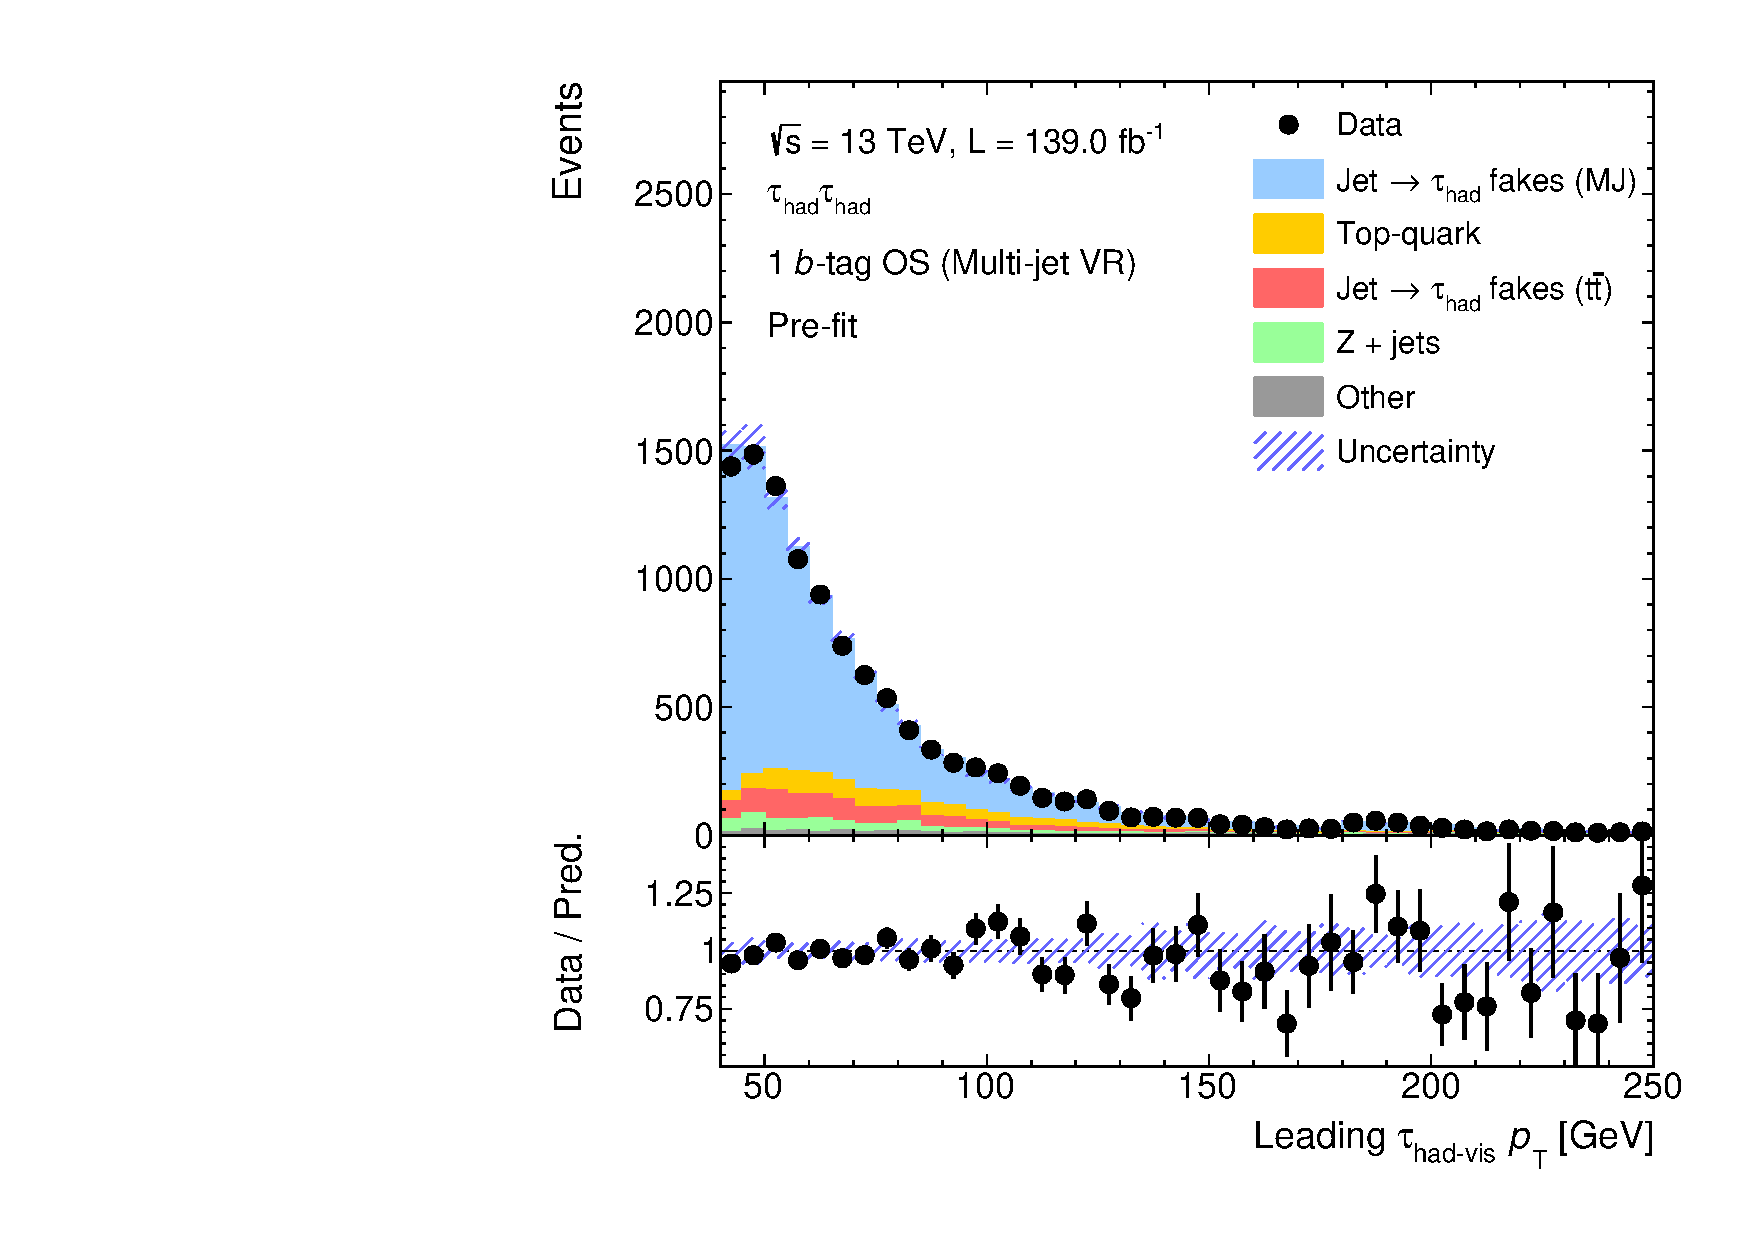
\includegraphics[width=\textwidth]{fakefactors/fake_os_vr/Tau0Pt_fakevr}
  \end{subfigure}\hspace*{0.04\textwidth}%
  \begin{subfigure}{0.45\textwidth}
    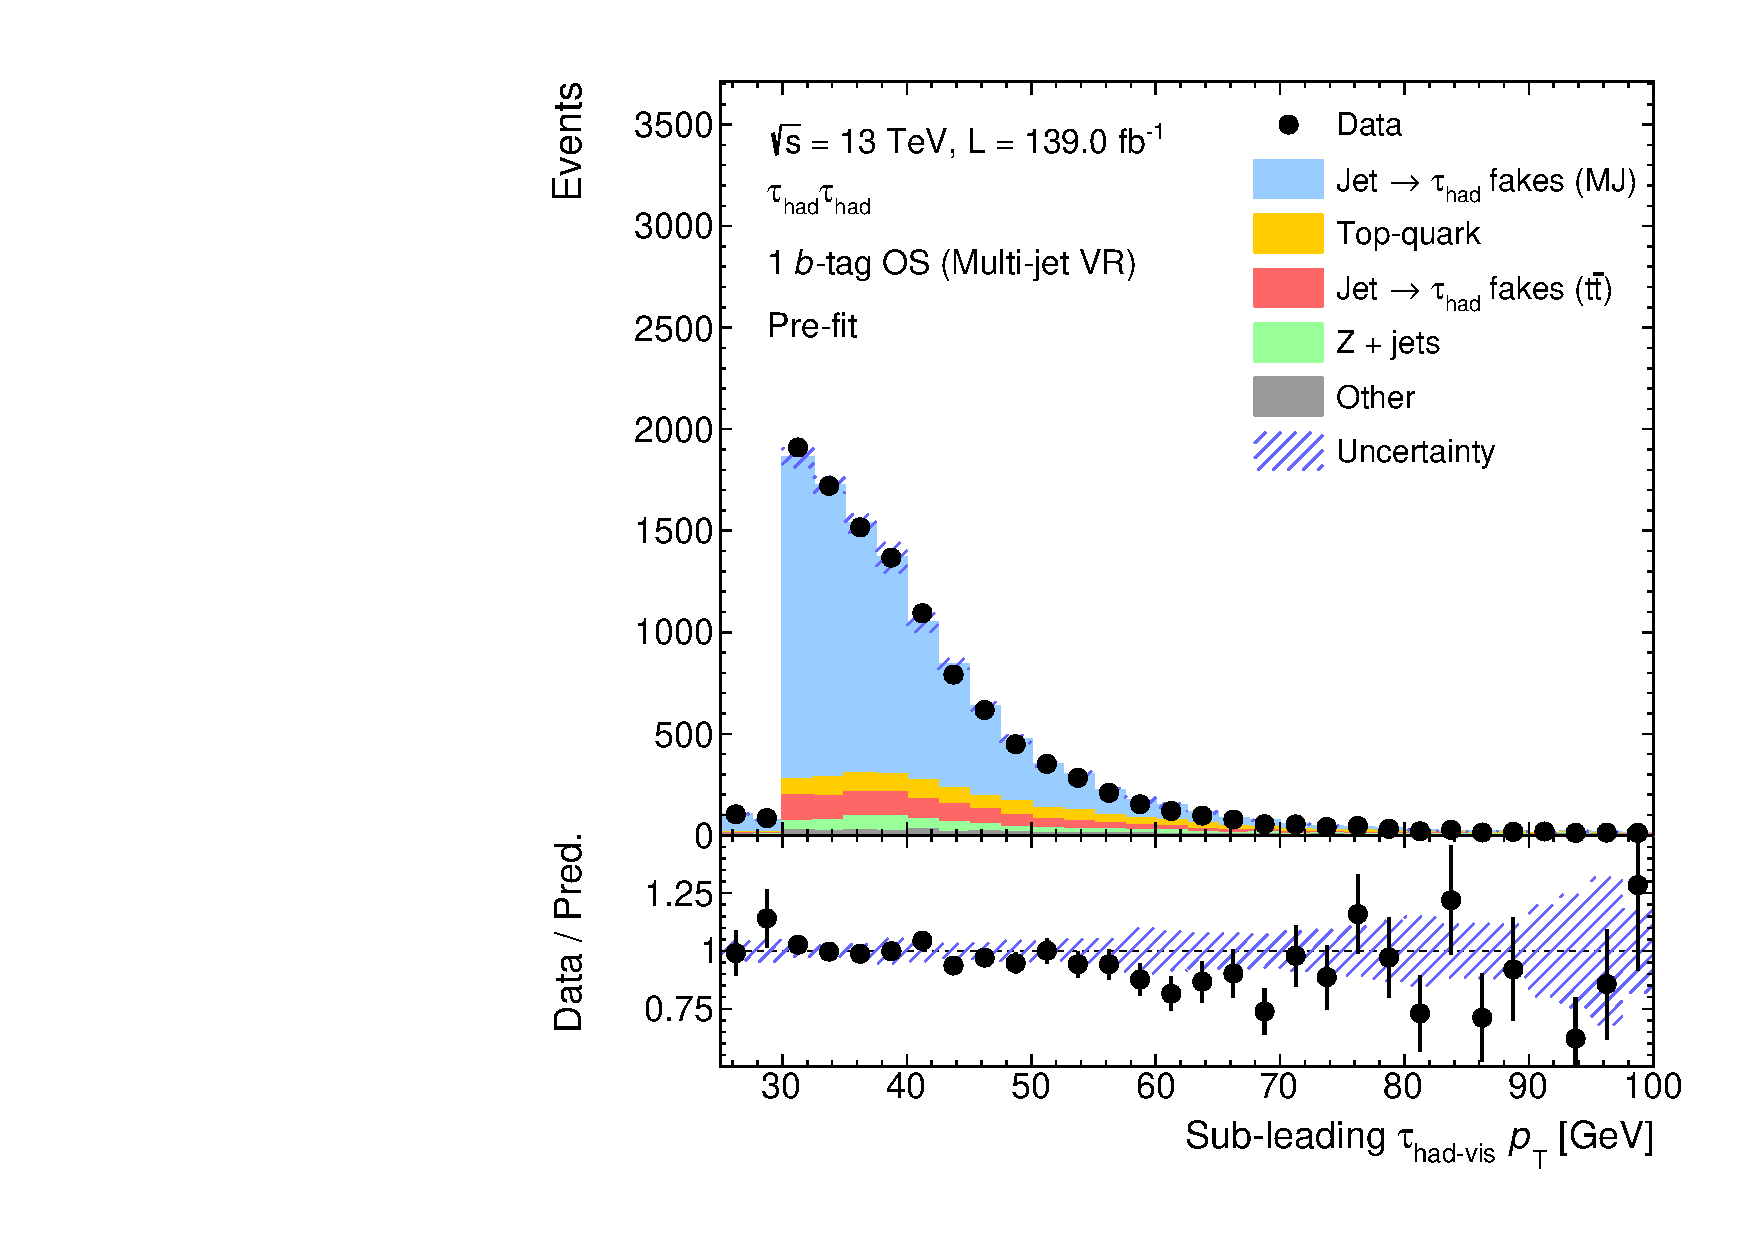
\includegraphics[width=\textwidth]{fakefactors/fake_os_vr/Tau1Pt_fakevr}
  \end{subfigure}

  \begin{subfigure}{0.45\textwidth}
    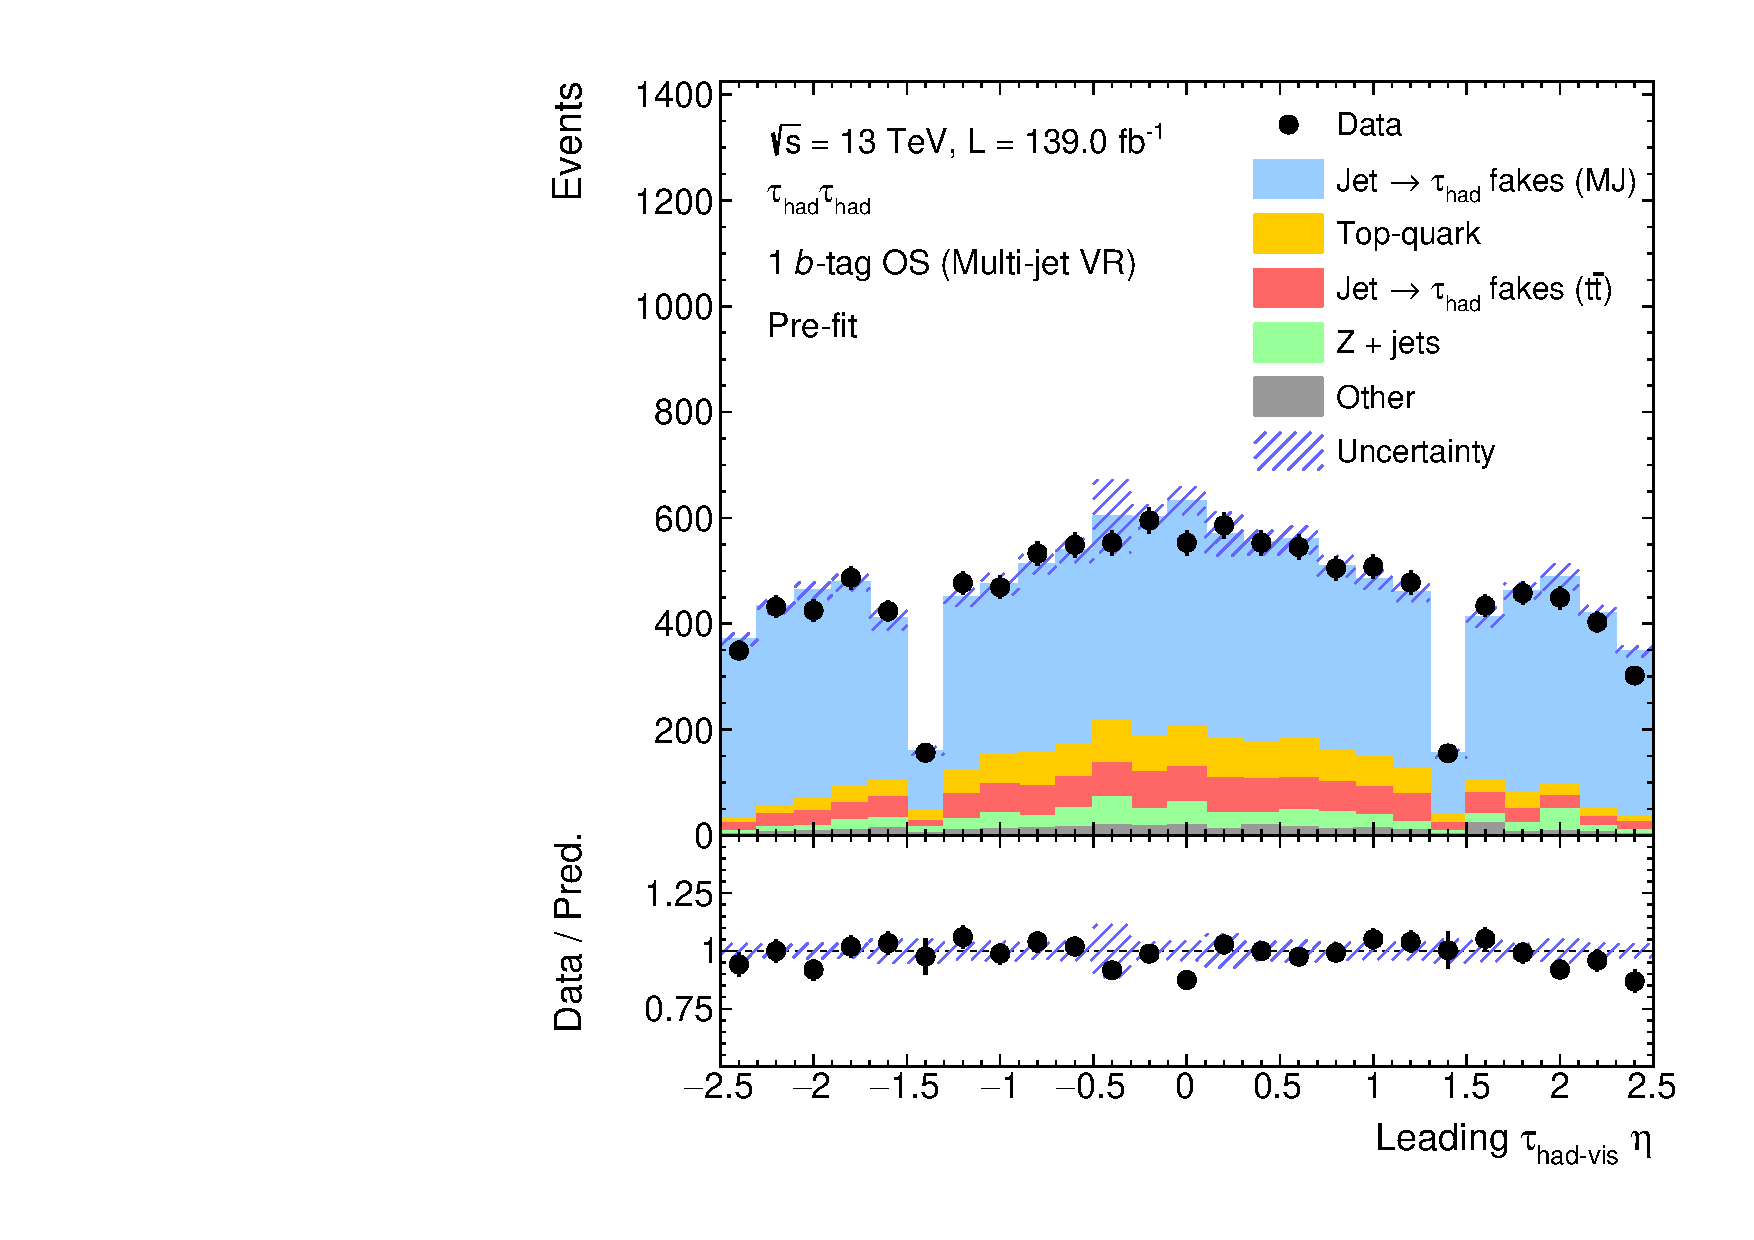
\includegraphics[width=\textwidth]{fakefactors/fake_os_vr/Tau0Eta_fakevr}
  \end{subfigure}\hspace*{0.04\textwidth}%
  \begin{subfigure}{0.45\textwidth}
    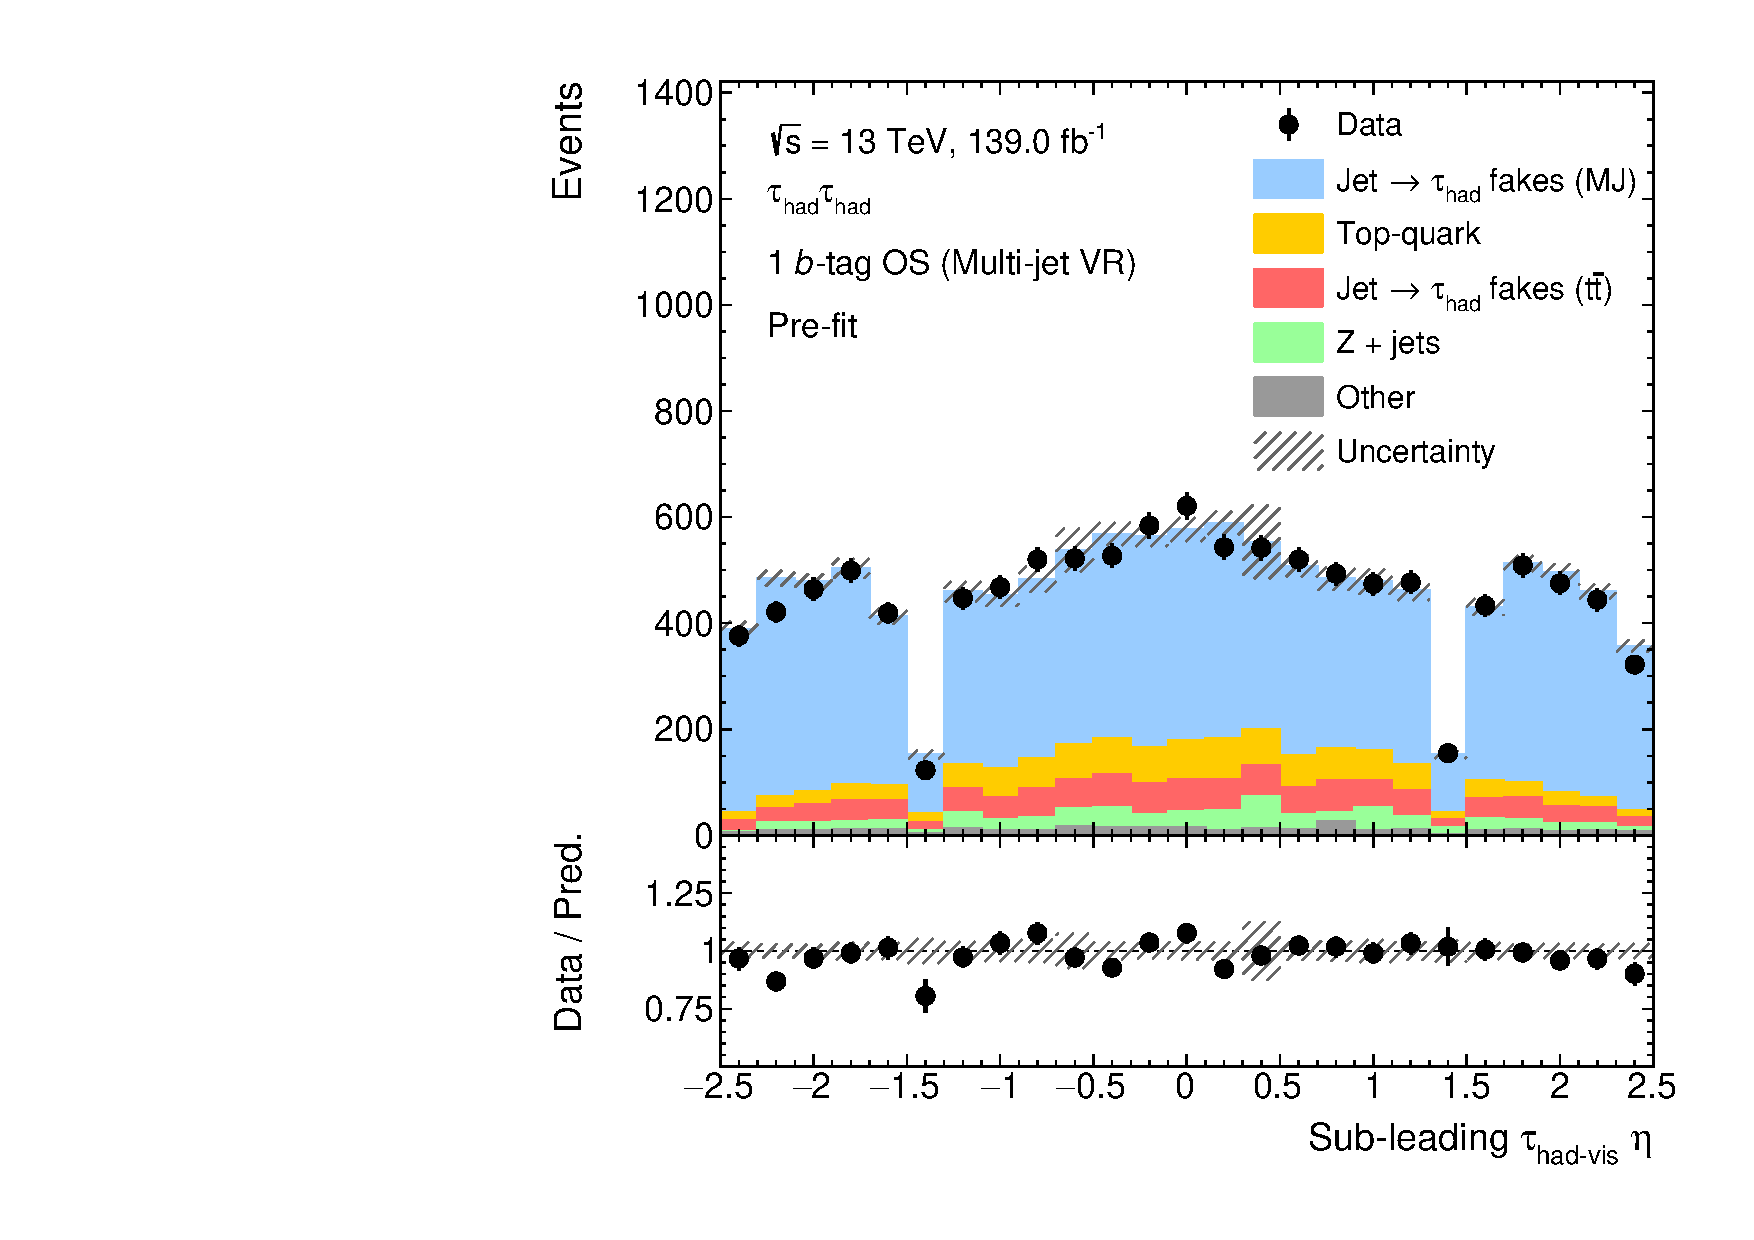
\includegraphics[width=\textwidth]{fakefactors/fake_os_vr/Tau1Eta_fakevr}
  \end{subfigure}

  \begin{subfigure}{0.45\textwidth}
    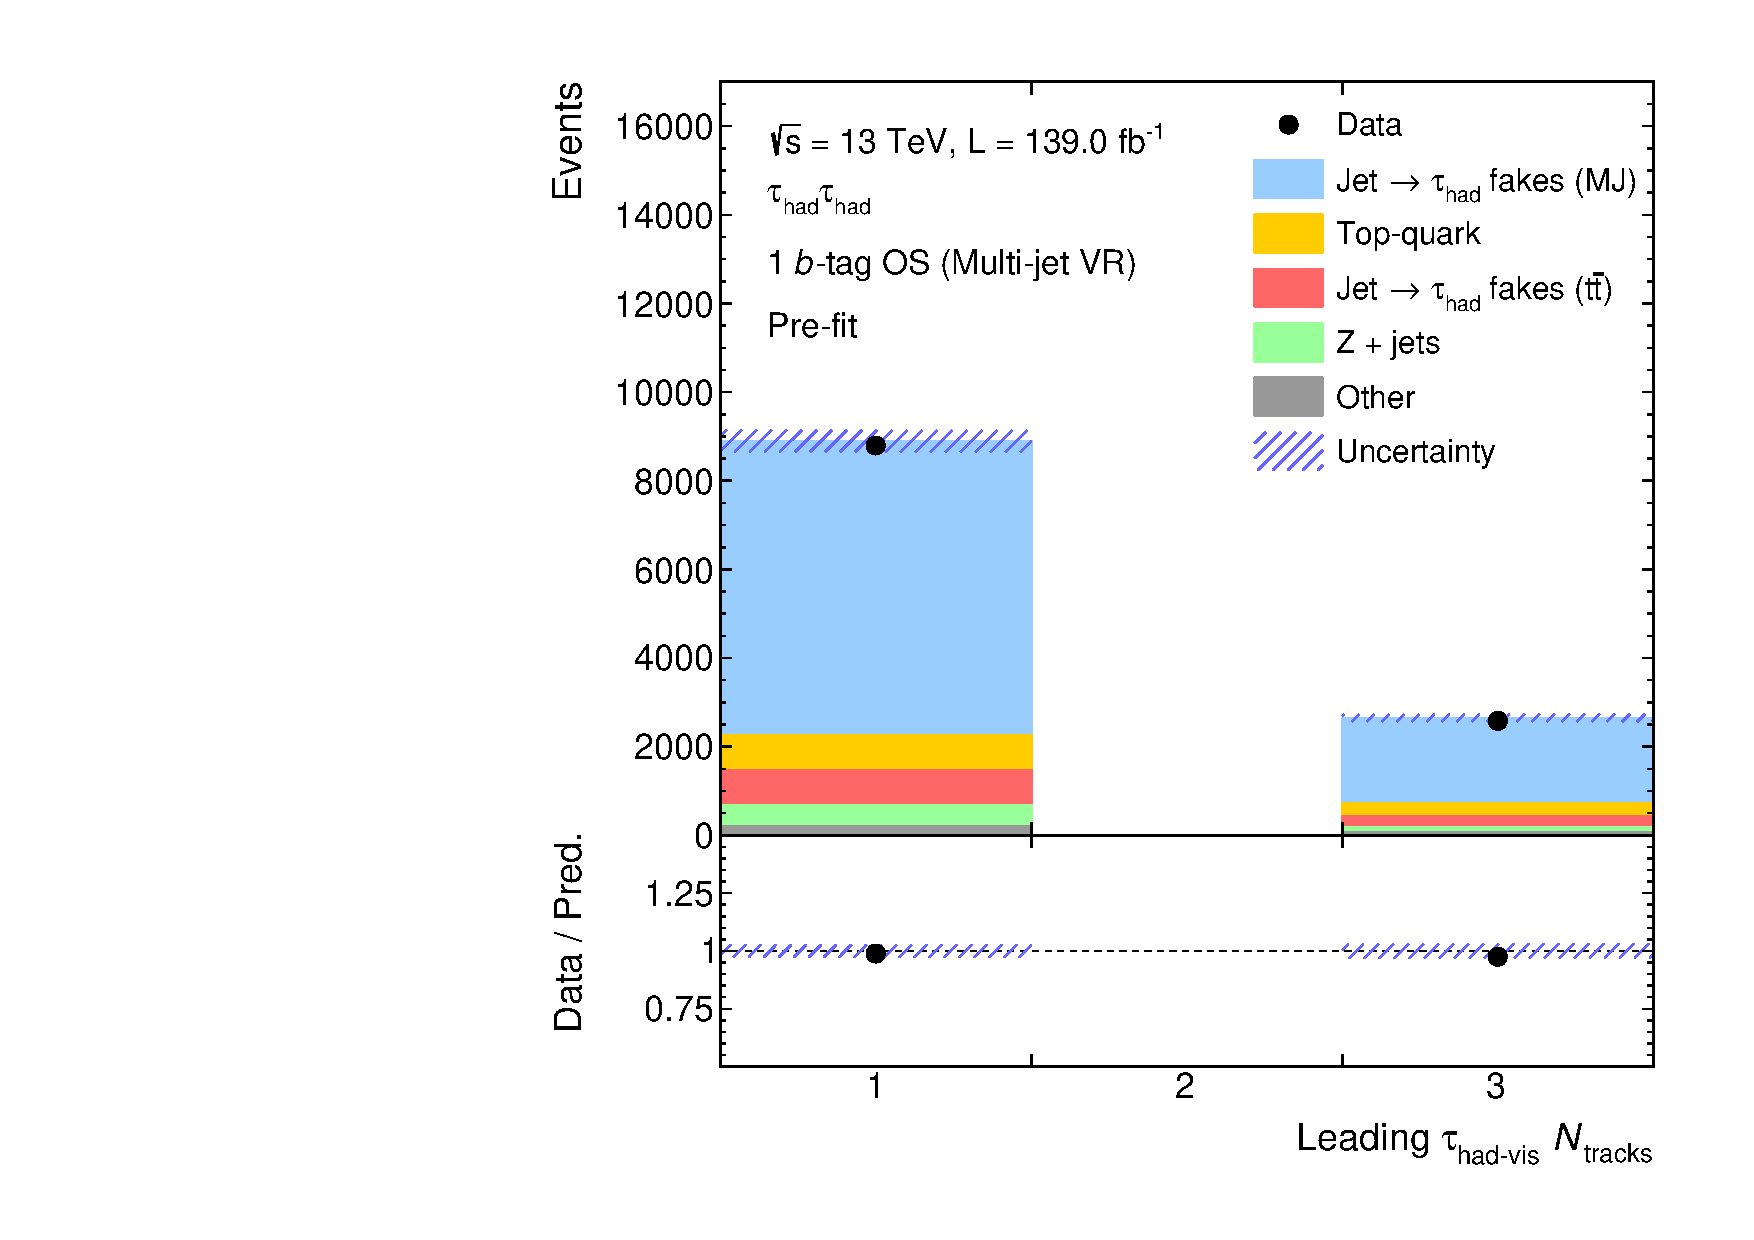
\includegraphics[width=\textwidth]{fakefactors/fake_os_vr/Tau0Ntrk_fakevr}
  \end{subfigure}\hspace*{0.04\textwidth}%
  \begin{subfigure}{0.45\textwidth}
    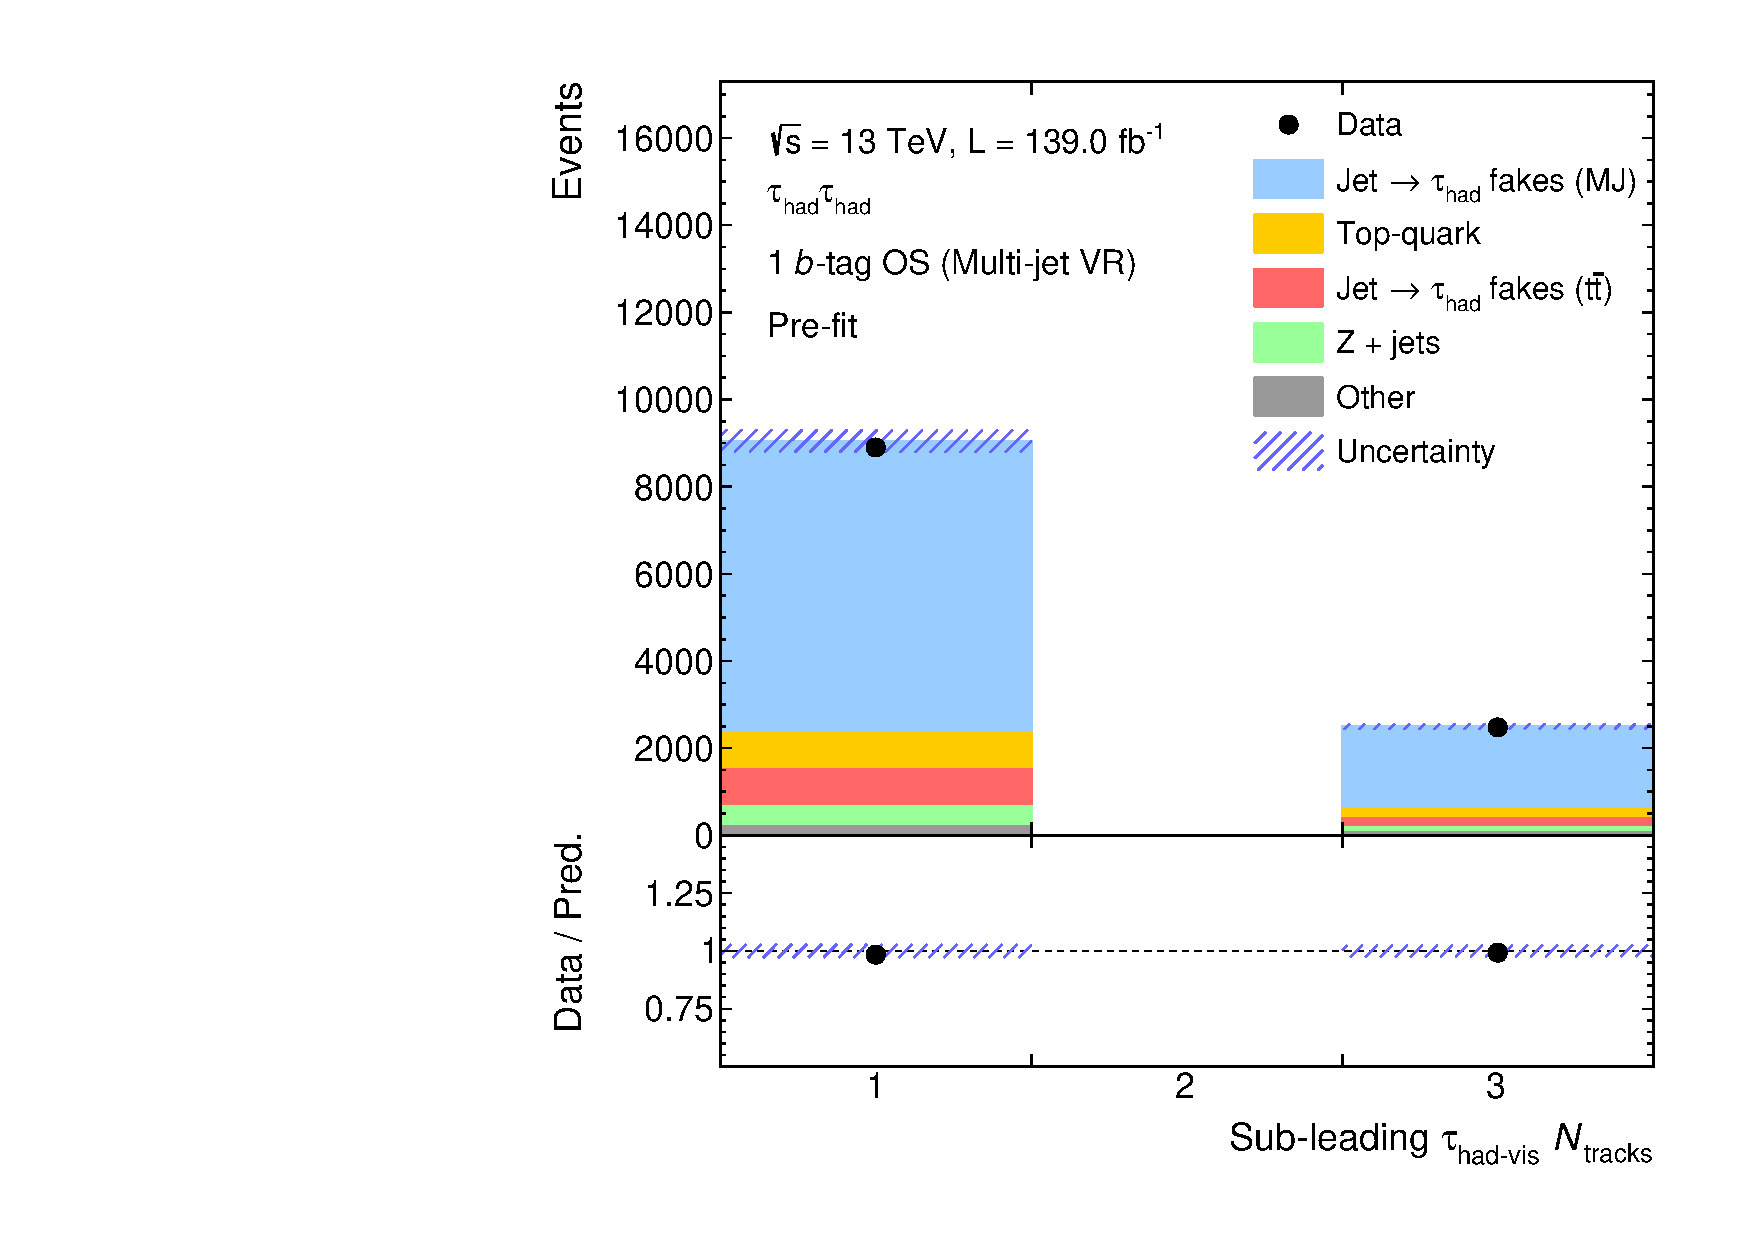
\includegraphics[width=\textwidth]{fakefactors/fake_os_vr/Tau1Ntrk_fakevr}
  \end{subfigure}

  \caption{Validation of \tauhadvis observables in the multi-jet VR (1
    $b$-tag OS, $\mMMC > \SI{110}{\GeV}$, and $\mathcal{S} < 3$). The
    estimate of the multi-jet background (light blue) is obtained
    using the fake factor method (cf.\
    \Cref{fig:fakefactor_regions}). Observables (top: \tauhadvis \pT,
    center: \tauhadvis $\eta$, bottom: \tauhadvis $N_\text{tracks}$)
    of the \tauhadvis candidates leading (left) and sub-leading in \pT
    (right) are shown. The background prediction is shown pre-fit,
    including statistical and detector-related systematic
    uncertainties.}%
  \label{fig:fake_factor_OSVR_kinematics}%
  % Explicitly say that there are no fake uncertainties here yet?
\end{figure}

Further tests of the assumptions can be performed by direct comparison
of fake factors previously measured in the 1 $b$-tag SS region with
the ones that would be obtained from a measurement in the 1 $b$-tag OS
multi-jet VR. Differences between both sets of fake factors can then
be applied as a non-closure uncertainty when applying fake factors
measured in SS regions in OS regions.

In~\Cref{fig:fake_factor_OSSS} a comparison of fake factors measured
in the 1 $b$-tag OS multi-jet VR and the 1 $b$-tag SS region is
shown.

Few events compared to SS and comparatively large subtraction -> large
statistical uncertainties.

The fake factors are compared using $\chi^2$-tests showing good
agreement with one exception. The di-\tauhadvis trigger fake factor
(2015-2016) for 3-prong \tauhadvis with \pT from
\SIrange{50}{65}{\GeV} in the endcaps of the ATLAS detector shows
significant deviations of \SI{50}{\percent} between OS and SS regions.


% Say something regarding the independence?

% Independence -> SS and OS fake factors have to agree
%
% measure OS fake factors in this region and add full difference as an uncertainty.

\begin{figure}[htbp]
  \centering

  \begin{subfigure}[t]{0.48\textwidth}
    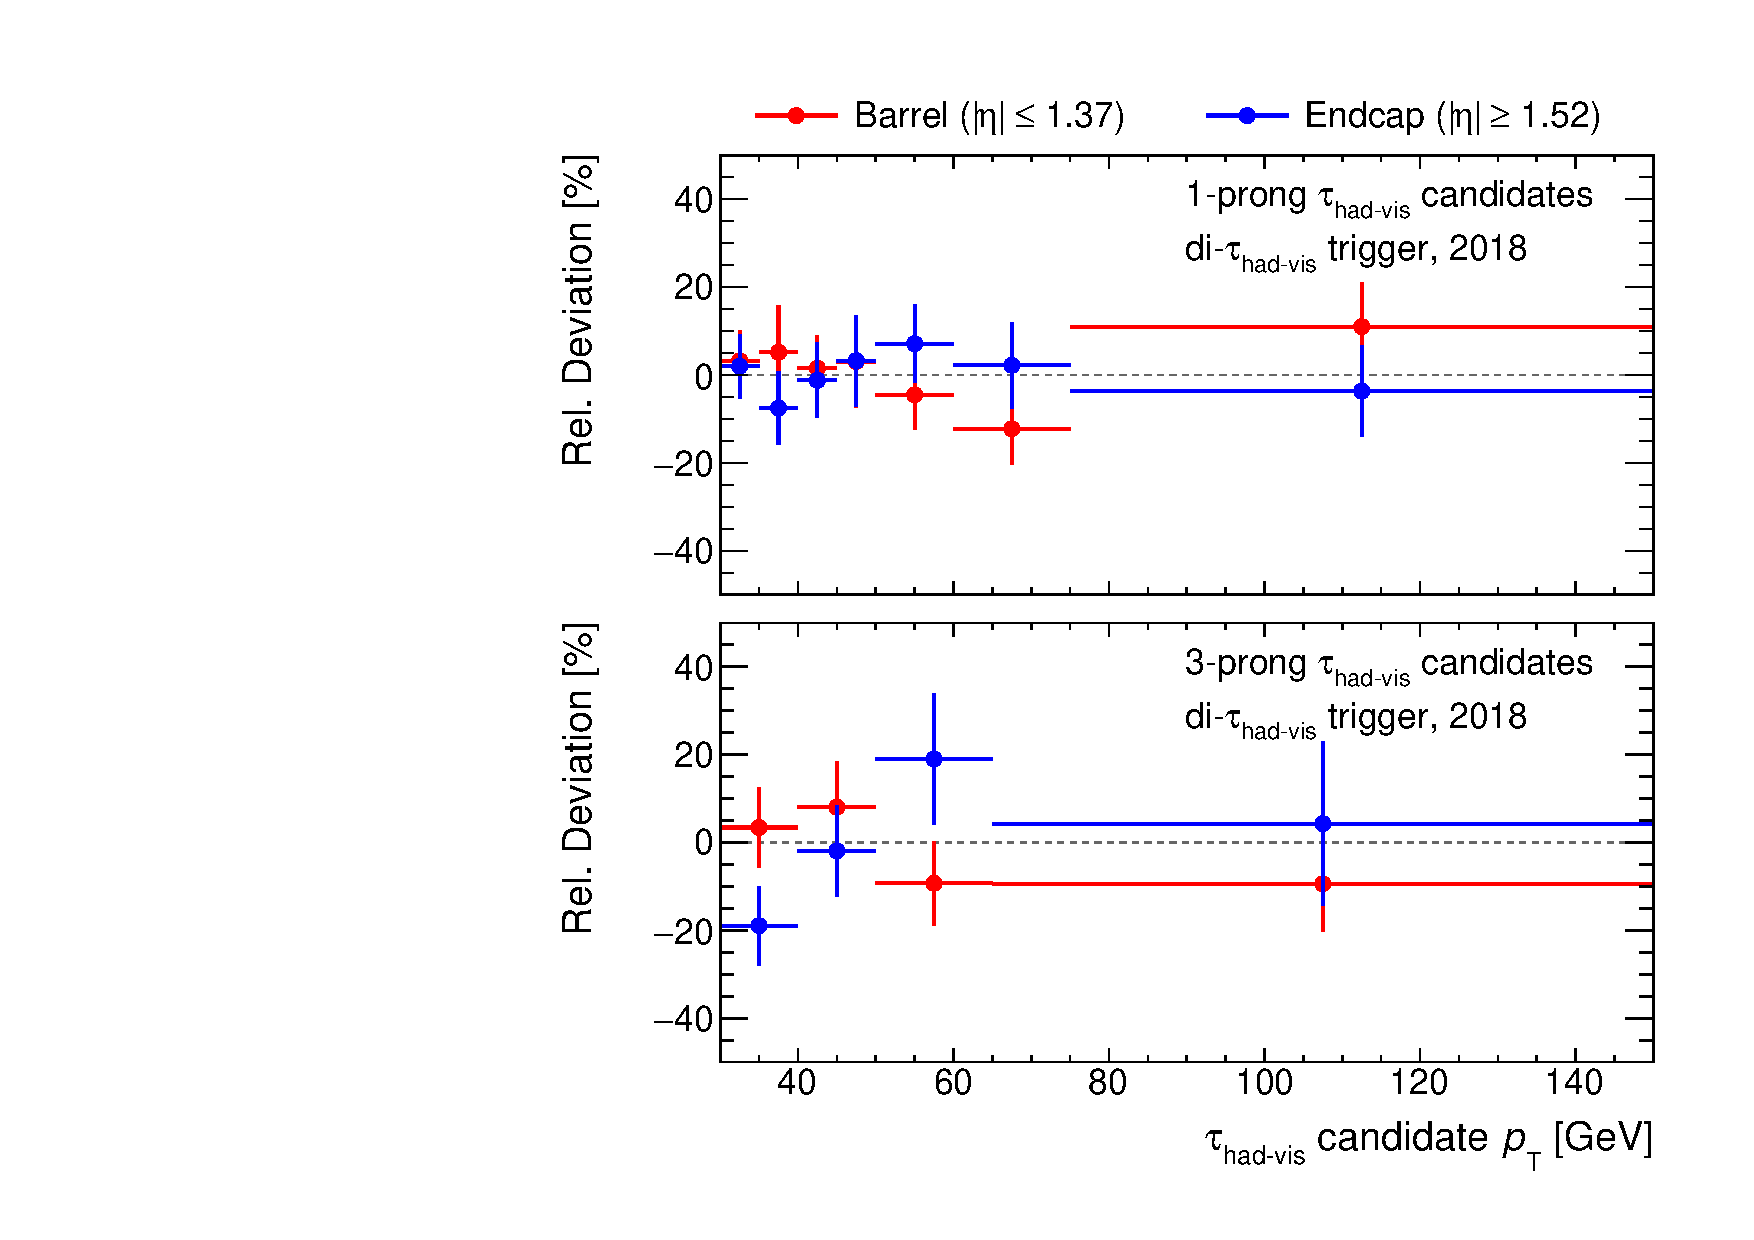
\includegraphics[width=\textwidth]{fakefactors/os_ss/fake_factors_osss_18}
    \subcaption{Comparison of OS and SS fake factors for events
      selected by di-\tauhadvis triggers. Only the 2018 data
      collection period is shown for illustration purposes.}
  \end{subfigure}\hfill%
  \begin{subfigure}[t]{0.48\textwidth}
    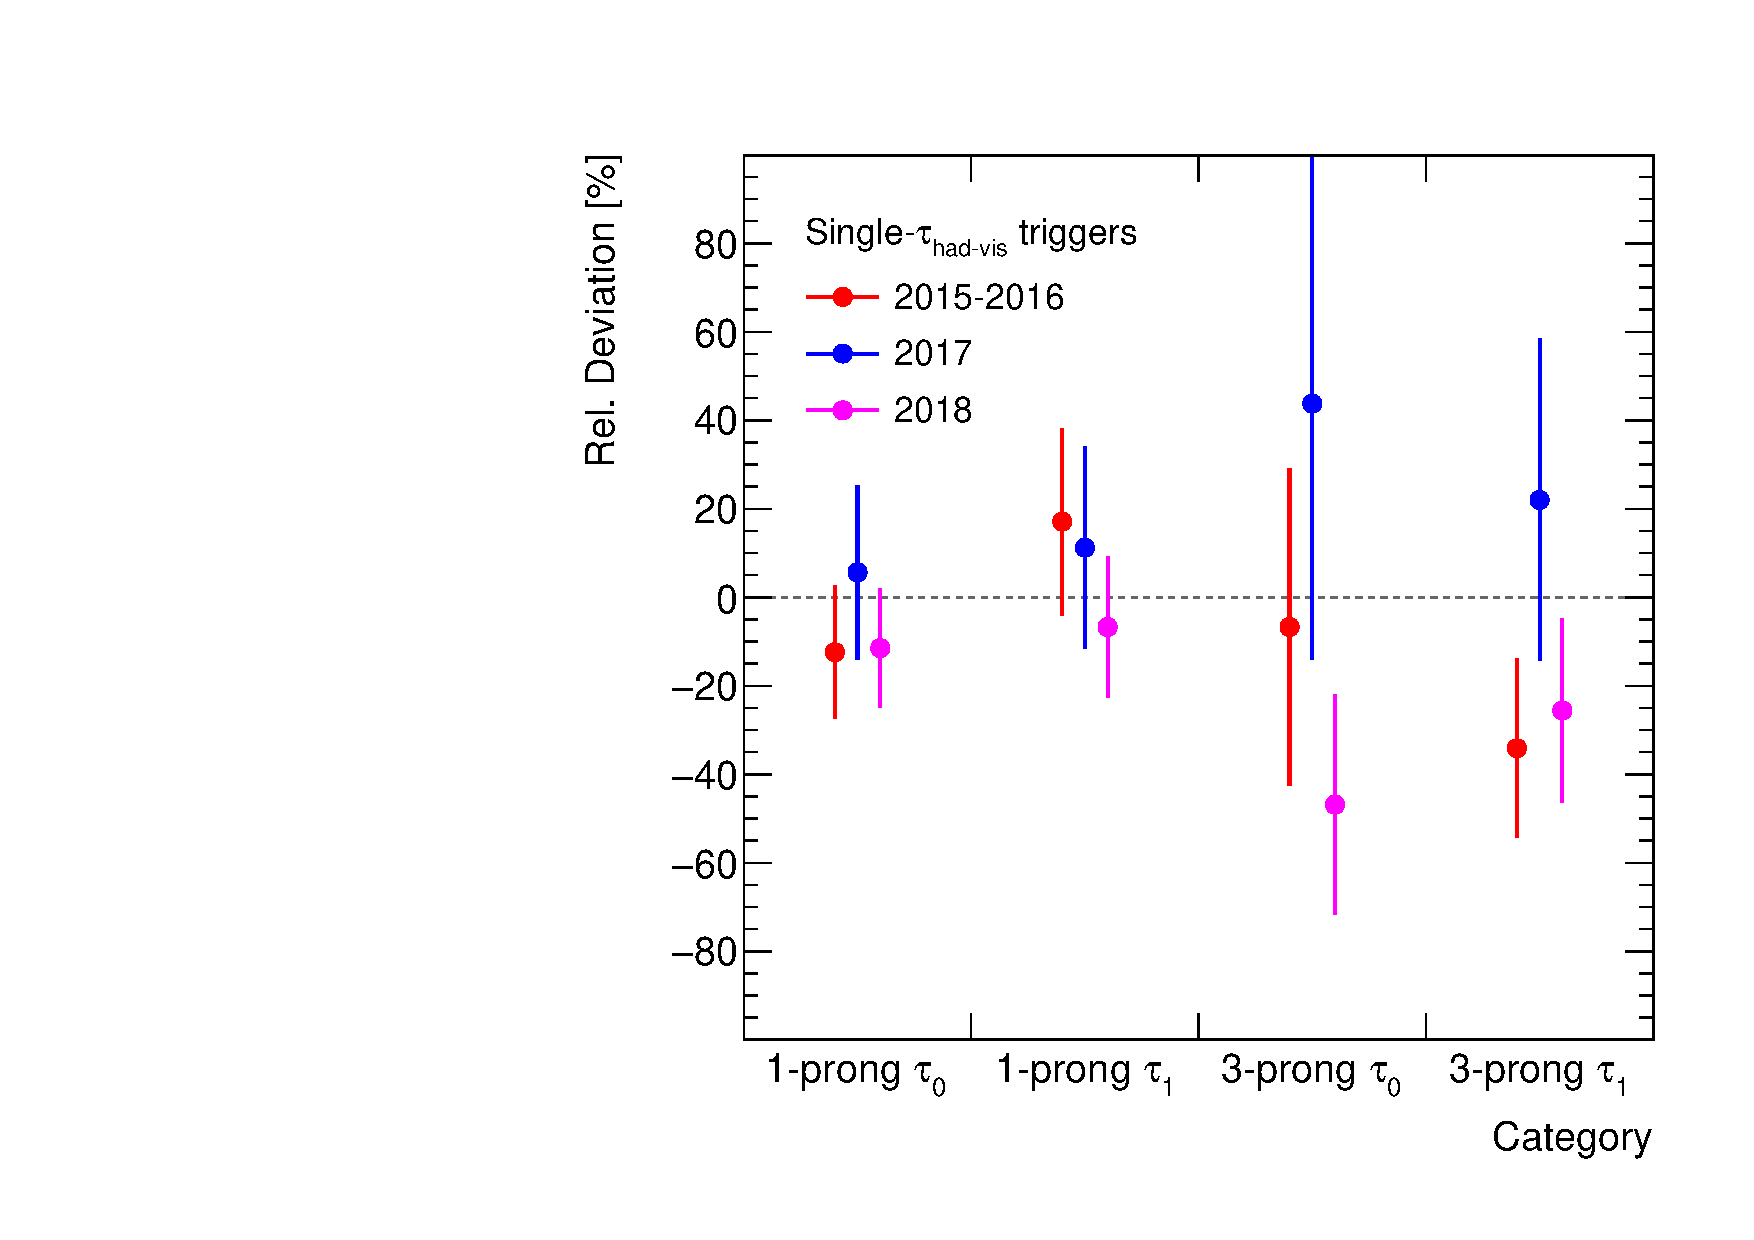
\includegraphics[width=\textwidth]{fakefactors/os_ss/fake_factors_osss_stt}
    \subcaption{Comparison of OS and SS fake factors for events
      selected by single-\tauhadvis triggers for all major data
      collection periods.}
  \end{subfigure}

  \caption{Relative deviation of fake factors measured in the 1
    $b$-tag OS multi-jet VR compared to the nominal set of fake
    factors measured in the 1 $b$-tag SS region (cf.\
    \Cref{fig:mjfakes_fake_factors,fig:mjfakes_stt_ffs}). The relative
    deviation is measured as $\FF_\text{OS} / \FF_\text{SS} - 1$ and
    is used to define a non-closure uncertainty that is propagated to
    the multi-jet background estimate when applying SS fake factors to
    events in OS regions. Statistical uncertainties from the finite
    number of observed data events and the non-multi-jet subtraction
    are shown.}
  \label{fig:fake_factor_OSSS}
\end{figure}




\subsubsection{Transfer factors}

The signal region is in 2 $b$-tag...

% Problems:
%
% - Very few events in SS region and high impurities from ttbar fakes
%   -> Only inclusive fake factors possible
%
%   - Transfer factor is determined by comparing the inclusive fake
%   factor calculated in 1-tag to an inclusive fake factor calculated
%   in 2-tag.
%
%   - Transfer factors show good agremeent between the 1- and 2-tag
%   region with large uncertainties
%
%   - Large uncertainties indicate that we have little sensitivity to
%   the differences between 1- and 2-tag regions.
%
%   - Therefore the 1-tag fake factors are used also in 2-tag region
%   after multiplying them by the transfer factor
%
%   - The primary aim of the transfer factor is to estimate an
%   uncertainty by coherently (conservative approach) varying the
%   transfer factors up and down separate for all four categories.



\subsubsection{Systematic Uncertainties}

% - Uncertainties


% The fake factors are not expected to depend strongly
% on the applied \btag requirement

% Dominant subtraction is ttbar, execpt for 1-tag OS ID where it is
% Ztautau.

% Signal contamination / other background contamination

% Yield table / plots of regions

% Checked in 1-tag OS. Does agreement in 1-tag OS confirm that charge
% and ID are independent? Closure, yes

\todo[inline]{Old stuff below:}

The fake factor (FF) measures the ratio of events with fake \tauhadvis in ID and
Anti-ID region:
\begin{align*}
  \FF = \frac{N\left( \text{fake} \, \tauhadvis, \text{ID} \right)}{N\left( \text{fake} \, \tauhadvis, \text{Anti-ID} \right)}
\end{align*}
The probability of a jet faking a \tauhadvis depends strongly on \tauhadvis \pT
and decay mode. Therefore, the fake factor is frequently parametrised in these
quantities. It is also affected by the \tauhadvis identification already applied
in the high-level \tauhadvis-triggers which also needs to be taken into account.

The fake factors are measured in the fake enriched SS-region by subtracting
non-fake-\tauhadvis background using their estimates from simulation:
\begin{align*}
  \FF_\text{SS} = \frac{N(\text{SS}, \text{ID}) - N_\text{non-fake}(\text{SS}, \text{ID})}{N(\text{SS}, \text{Anti-ID}) - N_\text{non-fake}(\text{SS}, \text{Anti-ID})}
\end{align*}
where $N$ is the total yield and $N_\text{non-fake}$ the yield of
non-fake-\tauhadvis backgrounds in the corresponding region.

To obtain the fake \tauhadvis estimate in the OS ID-region, the assumption is
made that the fake factors are independent of the reconstructed charge of the
fake \tauhadvis candidates. Therefore, the SS fake factors $\FF_\text{SS}$ are
applied to events in the OS Anti-ID region after subtracting any
non-fake-\tauhadvis contributions.
\begin{align*}
  N(\text{fake}, \text{OS ID}) = \FF_\text{SS} \times \left[ N(\text{OS}, \text{Anti-ID}) - N_\text{non-fake}(\text{OS}, \text{Anti-ID}) \right]
\end{align*}
Systematic uncertainties are assigned to
cover possible difference betwen OS and SS fake factors, varying the
subtraction in the OS Anti-ID region. Moreover, the fake factors are
independently varied by their statistical uncertainty.

Due to the limited acceptance of fake \tauhadvis in the 2 \btag region, the 1
\btag region is used to calculate the fake factors instead. The 1 \btag fake
factors are applied to the 2 \btag OS Anti-ID region and an additional 1 to 2
\btag transfer factor is applied.

The binning of the fake factors is dependent on the trigger that selected the
event. For STT events the fake factor is binned in whether the anti-\tauhadvis
is leading or subleading in \pT, and the decay mode of the \tauhadvis
($N_\text{track}$). Due to low statistics in the STT category the fake factors
are inclusive in \tauhadvis \pT. The \tauhadvis identification at the HLT is
only applied to one of the two \tauhadvis candidates affecting the probability
of jets faking \tauhadvis, motivating the binning in whether the leading /
subleading \tauhadvis fails the identification.

For DTT events, HLT \tauhadvis identification is applied to both \tauhadvis
candidates. Therefore, the fake factors do not need to distinguish between cases
where the leading and subleading \tauhadvis fails the loose identification. The
fake factors for DTT events are parametrised in the \pT and decay mode of the
the \tauhadvis candidate failing the identification requirement.

Moreover, all fake factors are binned by data-taking period (${\text{2015-2016},
  \text{2017}, \text{2018}}$) which takes into account the different triggers
being used to select events used for the analysis.

\todo[inline]{Could we use nOS to enhance statistics? Maybe flip the FF method
  so that we use events in SS ID to build the template instead of OS Anti-ID.}

\todo[inline]{Can we make the STT FF depend on the trigger-match instead of
  the leading / subleading binning?}









%%% Local Variables:
%%% mode: latex
%%% TeX-master: "../../phd_thesis"
%%% End:


\subsection{Fake-\tauhadvis Backgrounds in the \lephad Channel}%
\label{sec:bkg_lephad_combined_ff}
The estimation of \faketauhadvis backgrounds in the \lephad channels is outlined
in the following. A data-driven background estimation technique yielding a
combined estimate of the multi-jet and \ttbar background with a \faketauhadvis
is adopted. The method is an extension of the FF~method
% , previously introduced in \Cref{sec:hadhad_multijet},
that accounts for multiple sources of \faketauhadvis, differing in their
process-specific FFs.

Events in the \lephad channel in which the selected \tauhadvis candidate is an
\antitau define the Anti-ID region used for the FF method. Two CRs are defined
that are enhanced in multi-jet and \ttbar events, respectively. Both regions can
be divided into an ID and an Anti-ID region. These CRs are used to determine FFs
specifically for \faketauhadvis from multi-jet and \ttbar events. The CR
definitions and FF measurements are described in the following:
\begin{description}

\item[Multi-jet fake factors] are determined in a region defined by the
  requirement that the electron/muon fails the loose isolation working
  point. Moreover, the $\mBB < \SI{150}{\GeV}$ requirement is dropped. The
  remainder of the CR selection is identical to the SR selection of the \lephad
  channels. This CR has high multi-jet purity and allows calculating multi-jet
  FFs, \FFqcd, as the ratio of multi-jet events in the ID and Anti-ID
  region. The number of multi-jet events is estimated by subtracting the
  expected number of non-multi-jet events, which is estimated using simulation,
  from the observed number of events.

\item[\ttbar fake factors] are determined in a region defined by requiring
  $\mBB > \SI{150}{\GeV}$ with the other selections remaining identical to the
  SR selection. This CR has high \ttbar purity but is not pure in \ttbarFakes
  events due to contributions of \ttbar events with a \truetauhadvis that have
  to be subtracted. FFs for \ttbar, \FFttbar, are calculated as the ratio of
  \ttbarFakes events in ID and Anti-ID regions. The number of \ttbarFakes events
  is estimated, assuming negligible contribution of multi-jet events, by
  subtracting the expected number of non-\ttbarFakes events, which is estimated
  using simulation, from the observed number of events.

\end{description}
The FF measurement is performed separately for the \lephad SLT and LTT channels,
and separately for 1- and 3-prong \tauhadvis candidates. Moreover, the FFs are
measured in bins of \tauhadvis candidate \pT.

When estimating the \faketauhadvis background in one of the \lephad SRs, it
needs to be considered that the corresponding Anti-ID region consists of a
mixture of multi-jet and \ttbarFakes events. Let \rqcd be the fraction of
\faketauhadvis backgrounds that originate from multi-jet events in the Anti-ID
region. \emph{Combined fake factors} are defined as the weighted combination of
\FFqcd and \FFttbar:
\begin{align*}
  \FFcomb = \rqcd \, \FFqcd + (1 - \rqcd) \, \FFttbar \,\text{.}
\end{align*}
The combined FFs can be applied to events with \faketauhadvis, irrespective of
whether the event originates from multi-jet or \ttbar processes, to yield the
background estimate in the ID region. The determination of \rqcd proceeds
according to
\begin{align}
  \rqcd =
  \frac{N_{\text{multi-jet}}}{N_{\text{multi-jet}} + N_{\text{\ttbarFakes}}}
  = \frac
  { N_{\text{data}} - N_{\text{non-multi-jet}} }
  { N_{\text{data}} - N_{\text{non-(multi-jet or \ttbarFakes)}} } \,\text{,}
  \label{eq:rqcd}
\end{align}
where $N_{\text{data}}$ is the number of events observed in the Anti-ID region
and $N_{p}$ the number of events expected from process $p$ in the Anti-ID
region. The subtractions on the right-hand side of \Cref{eq:rqcd} use the
expected number of events predicted using simulation. This includes the
subtraction of \ttbarFakes events in the numerator.

The determination of \rqcd is performed separately for the \lephad SLT and LTT
channels, 1- and 3-prong \tauhadvis candidates, and events containing electrons
and muons. In addition, \rqcd is determined in bins of \pT of the \tauhadvis
candidate. In the SLT channel, \rqcd is typically small or zero showing that the
majority of \faketauhadvis backgrounds originate from \ttbar. The multi-jet
contribution in the LTT channel is larger with \rqcd ranging from
\SIrange{10}{30}{\percent} depending on \tauhadvis candidate \pT and
\Ntracks. Uncertainties on the \rqcd estimate have little impact on the
\faketauhadvis background prediction since \FFqcd and \FFttbar tend to be of
similar size in most bins.

The use of a similar method in the \hadhad channel would be preferred compared
to separately estimating the \faketauhadvis background from multi-jet and
\ttbar. The combined FF method does not need to distinguish between events with
\faketauhadvis from multi-jet and \ttbar when applying the FFs to events in the
Anti-ID region. In contrast, the multi-jet estimate in the \hadhad channel
requires a large subtraction of \ttbarFakes events, which is a dominant source
of systematic uncertainty. In the combined FF method this uncertainty is
restricted to an uncertainty on \rqcd. Despite possibly large uncertainties on
\rqcd, the uncertainty on the \faketauhadvis background estimate from the
combined FF method would be small since \FFqcd and \FFttbar are of similar
size. The search presented in this thesis is not limited by uncertainties
related to the \faketauhadvis background estimation and therefore this approach
was not pursued. However, in the future systematic uncertainties will become
more relevant at which point the combined FF method should also be considered
for the \hadhad channel.

% The \faketauhadvis estimation in the \lephad channel is concluded by briefly
% discussing the reason for not using a combined FF method in the \hadhad
% channel. In general, using a similar method in the \hadhad channel would be
% preferred compared to performing separate estimates of the \faketauhadvis
% backgrounds from multi-jet and \ttbar. This is because the combined FF method
% does not require to distinguish between events with \faketauhadvis from
% multi-jet and \ttbar when applying the FFs to events from the Anti-ID
% region. Currently, the multi-jet estimate in the \hadhad channel requires a
% large subtraction of \ttbar events with \faketauhadvis, which is a large
% source of systematic uncertainty on the multi-jet estimate. For the combined
% FF method, this uncertainty would be restricted to an uncertainty on the \rqcd
% determination. However, under the assumption that \FFqcd and \FFttbar are
% similar, a large uncertainty on \rqcd would only have a small effect on the
% resulting \faketauhadvis background estimate.

% Difficulties arise when trying to adopt the method to the \hadhad channel
% which were previously discussed in \Cref{sec:bkg_hadhad_ttbarfakes}. It is
% possible that these can be overcome in the future. At the current stage the
% search is not limited by uncertainties related to the \faketauhadvis
% estimation methods and therefore this approach was not pursued. However, the
% method should be considered for future iterations of this search for which
% systematic uncertainties will become more relevant.

%%% Local Variables:
%%% mode: latex
%%% TeX-master: "../../phd_thesis"
%%% End:



%%% Local Variables:
%%% mode: latex
%%% TeX-master: "../../phd_thesis"
%%% End:
